% Generated by md_to_tex_paper.py from ENTROPY_PRODUCTION.md -- do not edit by hand.
\documentclass[11pt,a4paper]{article}
\usepackage[T1]{fontenc}
\usepackage{lmodern}
\usepackage[margin=2.5cm]{geometry}
\usepackage{amsmath}
\usepackage{amssymb}
\usepackage{amsthm}
\renewcommand{\qedsymbol}{$\blacksquare$}
\usepackage{booktabs}
\usepackage{tabularx}
\usepackage{xltabular}
\usepackage{array}
\usepackage{enumitem}
\usepackage{tikz}
\usetikzlibrary{arrows.meta,positioning}
\usepackage{microtype}
\usepackage[hidelinks,pdfusetitle]{hyperref}

\setlength{\parskip}{0.45em}
\setlength{\parindent}{0pt}
\emergencystretch=4em
\hyphenpenalty=200
\renewcommand{\arraystretch}{1.12}
\allowdisplaybreaks
% A sentence that introduces a table is not left alone at the foot of a page: end the page first
% when fewer than seven lines remain (B50 Phase 2, 20 Sep 2026).  \pagegoal is \maxdimen on an
% empty page, so nothing happens there.
\newcommand{\keepwithtable}{\par\begingroup\dimen0=\pagegoal\advance\dimen0 by -\pagetotal
  \ifdim\dimen0<7\baselineskip\newpage\fi\endgroup}

% Theorem-like environments with the note's own numbers.  amsthm numbers automatically; the
% inner/outer pair below lets each instance carry its number by hand, so Theorem 0 stays 0 and
% nothing is renumbered.  Bodies are upright (definition style) so that the italic plain
% readings inside them stay italic and stand out.
\theoremstyle{definition}
\newtheorem{innertheorem}{Theorem}
\newenvironment{theoremx}[1]{\renewcommand\theinnertheorem{#1}\innertheorem}{\endinnertheorem}
\newtheorem{innerlemma}{Lemma}
\newenvironment{lemmax}[1]{\renewcommand\theinnerlemma{#1}\innerlemma}{\endinnerlemma}
\newtheorem{innerproposition}{Proposition}
\newenvironment{propositionx}[1]{\renewcommand\theinnerproposition{#1}\innerproposition}{\endinnerproposition}
\newtheorem{innerdefinition}{Definition}
\newenvironment{definitionx}[1]{\renewcommand\theinnerdefinition{#1}\innerdefinition}{\endinnerdefinition}
\newtheorem{innerremark}{Remark}
\newenvironment{remarkx}[1]{\renewcommand\theinnerremark{#1}\innerremark}{\endinnerremark}
\newtheorem{innercorollary}{Corollary}
\newenvironment{corollaryx}[1]{\renewcommand\theinnercorollary{#1}\innercorollary}{\endinnercorollary}

\title{One-way functions are computational entropy production}
\author{Casey Thornton \\ Independent researcher \\ caseythornton@utexas.edu}
\date{Version of 20 September 2026}
\hypersetup{pdfauthor={Casey Thornton}}

\begin{document}
\maketitle
\thispagestyle{plain}


\section*{Abstract}
\phantomsection\addcontentsline{toc}{section}{Abstract}

One-way functions exist if and only if some efficiently samplable process produces more than logarithmic computational entropy on average, for infinitely many input lengths. We make this precise. For a polynomial-time samplable distribution $D$ on pairs $(x, y)$, the computational entropy production of a pair is $\sigma$ = log $D(x, y)$ + $\mathrm{pK}^t(y) + \mathrm{pK}^t(x \mid y)$, where $\mathrm{pK}^t$ is the probabilistic time-bounded Kolmogorov complexity as defined by Hirahara, Ilango, Lu, Nanashima and Oliveira (2023, HILNO below) following Goldberg, Kabanets, Lu and Oliveira (2022): the log-probability the process assigns to the pair, against the length of a bounded observer's shortest fast description of it, output first, then input given output. We prove unconditionally that $\mathrm{E}_D[2^{-\sigma}]$ lies between an inverse polynomial and a polynomial in $n$ and that $\mathrm{E}_D[\sigma] \ge -O(\log n)$: a time-bounded fluctuation inequality and a computational second law. We show that, up to a polynomial and outside a $1/n$ slice of outputs, $\sigma$ is small on a pair exactly when an efficient sampler, given the output, recovers the input with about the right odds, HILNO's universal sampler serving as the witness: dissipation, in this sense, is the hardness of running the process backward. The equivalence in the first sentence is HILNO's duality restated in these terms, for infinitely-often one-way functions. For the antisymmetric Zurek defect, one-way functions force superpolynomial exponential moments, and bounded moments sit between $\mathrm{NP} \subseteq \mathrm{BPP}$ and the non-existence of one-way functions; whether the lower arrow reverses is left open, with a conditional relativization barrier on that arrow and oracle evidence on the other. Physics is the frame, not the subject.

\emph{Plain reading of the abstract: a fast random process makes pairs. Ask an observer with limited time to tell the story of each pair backwards, output first. The paper counts how many more bits that backward story costs than the process itself paid. Two easy facts about short descriptions show that this cost is, on average, never much below zero, for every fast process, with no assumptions. A known theorem then says the cost is large on average for some fast process exactly when one-way functions exist. A further result says the cost is small on a pair exactly when a fast machine, shown the output, can guess the input with about the right odds: dissipation is the hardness of running the process backward. The remaining result compares the two directions of description and shows that one-way functions make that two-sided comparison blow up; whether the reverse holds is left open, and so is which world we live in.}

\keepwithtable

\textbf{Results.} The four theorems and their standing.

\par\medskip\noindent
{\small
\begin{xltabular}{\textwidth}{@{}>{\hsize=0.40\hsize\raggedright\arraybackslash}X>{\hsize=1.65\hsize\raggedright\arraybackslash}X>{\hsize=0.95\hsize\raggedright\arraybackslash}X@{}}
\toprule
 & statement & standing \\
\midrule
\endhead
Theorem 1 & For every polynomial-time samplable process, unconditionally: $\mathrm{E}_D[2^{-\sigma}]$ lies between an inverse polynomial and a polynomial in $n$, and $\mathrm{E}_D[\sigma] \ge -O(\log n)$. & new \\
\addlinespace[3pt]
Theorem 2 & One-way functions exist iff some polynomial-time samplable process has mean production above $c \log n$ for infinitely many $n$, for every constant $c$. & restated: HILNO Theorem 1 \\
\addlinespace[3pt]
Theorem 3 & One-way functions force superpolynomial exponential moments of the same-time Zurek defect, infinitely often; $\mathrm{NP} \subseteq \mathrm{BPP}$ $\Rightarrow$ bounded moments $\Rightarrow$ no one-way functions. & assembled: HILNO's Lemma 20 argument and HILNO's Theorem 4, with the Kraft sums of Section 3 \\
\addlinespace[3pt]
Theorem 4 & $\sigma$ is small on a pair iff the universal sampler inverts it with the right odds, up to a polynomial and outside a $1/n$ slice. & assembled: HILNO Proposition 22, Lu--Oliveira--Zimand coding theorem \\
\bottomrule
\end{xltabular}}
\par\medskip

\section*{1. Introduction}
\phantomsection\addcontentsline{toc}{section}{1. Introduction}

Crooks's fluctuation theorem [Crooks 1999] is two lines long once its object is defined. Define the entropy production of a path as the log of the probability of that path under the forward process divided by the probability of the reversed path under the reverse process. Then the exponential average of minus the entropy production, over forward paths, is the total probability of the reverse process, which is one; and Jensen's inequality turns that identity into the second law, that the mean entropy production is not negative.

This paper carries out the same two lines with a polynomial-time sampler in the role of the forward process and a bounded observer's shortest fast description in the role of the reverse process. The description length is the probabilistic time-bounded Kolmogorov complexity $\mathrm{pK}^t$, as defined in [Hirahara, Ilango, Lu, Nanashima and Oliveira 2023, eq. (6)], written HILNO below. The computational entropy production of a sampled pair is the log of the sampler's probability of the pair over the weight the observer's shortest fast description gives it, output first, then input from output. Four things come out.

\begin{itemize}[leftmargin=1.2em,itemsep=3pt,topsep=3pt,parsep=0pt]

\item \textbf{Theorem 1.} The exponential average of minus the computational entropy production lies between an inverse polynomial and a polynomial in $n$ (the inverse polynomial depending on the sampler), and the mean is at least $-O(\log n)$, for every polynomial-time samplable process, unconditionally. The proof is two Kraft sums, one explicit pair and Jensen's inequality.

\item \textbf{Theorem 2.} One-way functions exist (infinitely-often, the notion used throughout) if and only if some polynomial-time samplable process has, for every constant $c$, mean computational entropy production above $c \log n$ for infinitely many $n$. This is HILNO's Theorem 1 read in the vocabulary of Theorem 1; it is a restatement, not a new theorem.

\item \textbf{Theorem 3.} For the difference of the two one-sided productions of a pair, the Zurek defect, the existence of one-way functions forces both exponential moments to be superpolynomial infinitely often; whether the converse holds is the paper's open problem, Question 1.

\item \textbf{Theorem 4.} Up to a polynomial and outside a $1/n$ slice of outputs, a process has small computational entropy production on a pair exactly when a fast machine, handed the output, can guess the input with about the right odds, and the universal sampler always serves as the witness. It is assembled from known parts, HILNO's universal sampler and the coding theorem with an auxiliary input, and its content is the identification: dissipation in this paper's sense is the failure of the reverse conditional to be dominated by an efficient sampler (Section 6).

\end{itemize}

\keepwithtable

Five rows of the correspondence the paper runs on, in the order the objects appear:

\par\medskip\noindent
{\small
\begin{xltabular}{\textwidth}{@{}>{\hsize=1.00\hsize\raggedright\arraybackslash}X>{\hsize=1.00\hsize\raggedright\arraybackslash}X@{}}
\toprule
Crooks [1999] & this paper \\
\midrule
\endhead
forward process: the forward path probability, $\rho_F(x_{-\tau})\, P[x(+t) \mid \lambda(+t)]$ & $D(x, y)$, the sampler's joint probability (Definition 2) \\
\addlinespace[3pt]
reverse process: the reverse path probability, $\rho_R(x_{+\tau})\, P[x(-t) \mid \lambda(-t)]$ & $m_R(x, y) = 2^{-\mathrm{pK}^t(y) - \mathrm{pK}^t(x \mid y)}$, the bounded observer's shortest fast description of the pair, output first (Definition 4) \\
\addlinespace[3pt]
entropy production $\omega = \log(\text{forward} / \text{reverse})$, eq. (7) & $\sigma^{\mathrm{rev}}_D = \log(D / m_R)$ (Definition 5) \\
\addlinespace[3pt]
integral fluctuation theorem, eq. (4): $\langle e^{-\omega}\rangle$ = 1 & $n^{-O(1)} \le \mathrm{E}_D[2^{-\sigma}] \le O(n^2)$ (Theorem 1(a)) \\
\addlinespace[3pt]
second law, $\langle\omega\rangle \ge 0$, by Jensen & $\mathrm{E}_D[\sigma] \ge -O(\log n)$ (Theorem 1(b)) \\
\bottomrule
\end{xltabular}}
\par\medskip

The full seventeen-row correspondence is Appendix A.1.

The route of the paper in one line, with the standing of each arrow:
\[
\begin{aligned}
&\text{some polynomial-time samplable process has mean production} \ge \omega(\log n) \text{ i.o.} \\
&\qquad\Leftrightarrow\;\; \text{one-way functions exist} \;\;\Rightarrow\;\; \mathrm{P} \ne \mathrm{NP}.
\end{aligned}
\]

\emph{Plain reading: a fast process that dissipates, in the sense defined in Section 2, is the same thing as a one-way function (Theorem 2), and a one-way function forces $\mathrm{P} \ne \mathrm{NP}$ (standard, Section 2.3, and not known to reverse); Theorem 1 says the left-hand quantity cannot be very negative for any process, and Theorem 3 refines it by a second, antisymmetric quantity and leaves one direction open.}

What is new and what is restated, in one sentence: the time-bounded fluctuation inequality of Theorem 1 and the reading of HILNO as mean entropy production in Theorem 2 were found in no source, while the interpretation in Section 9 adds nothing beyond what [Aaronson 2005, \S{}10], [Aaronson 2016a, footnote 20] and [Aaronson, Kardes and Hartle 2025, slide 27; unpublished] already say, and it says so.

The unbounded-time ancestor of Theorem 1 is in print: for ordinary Kolmogorov complexity, the chain Kraft's inequality, then an integral fluctuation inequality, then Jensen, is [Ebtekar and Hutter 2024, Lemma 5, Theorem 7 and eq. (44)]. Nothing in that work has a time bound, and one-way functions do not appear in it. The time-bounded version, and its cryptographic reading, are the content here.

Whether any polynomial-time samplable process dissipates in the sense of Theorem 2, that is, which of the five worlds we live in, is open, and this paper does not claim to decide it.

The audience is complexity theorists. A reader who skips every sentence about physics loses nothing from the theorems.

\subsection*{1.1 What the results are not}
\phantomsection\addcontentsline{toc}{subsection}{1.1 What the results are not}

Theorems 1, 2 and 4 hold in every one of Impagliazzo's five worlds [Impagliazzo 1995]; in Pessiland, where $\mathrm{P} \ne \mathrm{NP}$ and no one-way function exists, Theorem 2 says that every polynomial-time samplable process has mean production at most $O(\log n)$, so the dissipation statement is not a restatement of $\mathrm{P} \ne \mathrm{NP}$: the two are not known to be equivalent, and in Pessiland they would have different truth values. Theorem 3 does not decide which world holds, and no sentence of the paper claims that a physical process dissipates. Question 1 (Section 8) is not shown to be hard, only immune to relativizing proof for the bottom arrow of the same-time sandwich, $\text{no io-OWF} \Rightarrow \mathrm{BEM}$ (Proposition 10, conditional as stated there). For the top arrow the relativization test has been run only on the natural test distributions of two errorless worlds (Proposition 11, informal); whether same-time $\mathrm{BEM}$ holds relative to either oracle is open, so no barrier statement is made for that arrow. Read as a principle, the assumption, in its quantum-secure form (one-way functions secure against quantum algorithms), predicts that no efficiently measurable observable is a complexity meter, an instrument whose reading tracks the circuit complexity or the description length of the state it is applied to (an inference, not proved here: the sentence identifies ``efficiently measurable'' with ``implemented by a polynomial-size quantum circuit'', the quantum form of the extended Church--Turing thesis, an identification made here and nowhere else in the paper, Theorems 1 to 4 being stated for $\mathrm{BPP}$ samplers (\S{}7); and its general form rests on the existence of pseudorandom quantum states under quantum-secure one-way functions, Ji, Liu and Song 2018). The field has proved this one observable at a time: pseudoentanglement for entanglement entropy [Aaronson, Bouland, Fefferman, Ghosh, Vazirani, Zhang and Zhou 2024, Corollary 1.0.1], and pseudochaotic dynamics for the out-of-time-order correlator, whose Theorem 1 is unconditional [Lee, Kwon and Cho 2025, Theorem 1]. So the principle's only observational signature is the continued absence of the instrument.

\emph{Plain reading: the two main theorems are true no matter which of the five possible worlds we live in. In the world where hard problems exist but nothing is one-way, Theorem 2 says nothing dissipates; so ``something dissipates'' is not ``hard problems exist'' in new words, and nobody knows whether the two are equivalent. The paper does not say which world is real, does not say that any physical thing dissipates, and does not show its open problem is hard, only that one family of proof methods cannot deliver the bottom arrow; for the top arrow nothing of the kind is shown. And the assumption, read as a law about the world, predicts that no lab instrument can read how complex a state is: such an instrument would tell a cheaply made fake apart from a truly random state, which the assumption says nothing efficient can do, if fast measurements are fast quantum circuits. Physicists have been proving this one instrument at a time; so the only thing the principle shows the laboratory is the instrument that keeps not existing.}

\subsection*{1.2 How to read this paper}
\phantomsection\addcontentsline{toc}{subsection}{1.2 How to read this paper}

Three pages carry the claim: Section 1 (the chain and the four theorems), Section 2.5 (the definition of computational entropy production) and Section 9.2 (what it measures: lost against hidden). The proofs are Sections 3 to 6. Section 8 is the open problem, Question 1, and its placement, and can be skipped on a first reading. Section 9 is the physics frame, every sentence of it a labelled parallel. Every displayed formula is followed by an italic \emph{plain reading} that says what it means in words; a reader who does not want the notation can read the theorem statements and the plain readings alone.

\keepwithtable

The objects, in the order they appear:

\par\medskip\noindent
{\small
\begin{xltabular}{\textwidth}{@{}>{\hsize=0.72\hsize\raggedright\arraybackslash}X>{\hsize=0.90\hsize\raggedright\arraybackslash}X>{\hsize=0.62\hsize\raggedright\arraybackslash}X>{\hsize=1.76\hsize\raggedright\arraybackslash}X@{}}
\toprule
symbol & name & where & in plain words \\
\midrule
\endhead
$\mathrm{pK}^t$($x$), $\mathrm{pK}^t(x \mid y)$ & probabilistic time-bounded description length & Definition 1 & the fewest bits a fast program needs to print $x$, or $x$ given $y$, with a shared random string \\
\addlinespace[3pt]
$D(x, y)$ & samplable pair distribution & Definition 2 & the fast process; its probability of producing the pair (input $x$, output $y$) \\
\addlinespace[3pt]
io-OWF & infinitely-often one-way function & Definition 3 & a fast function no fast algorithm inverts on a noticeable fraction of inputs, for infinitely many lengths \\
\addlinespace[3pt]
$m_R$, $m_F$ & reverse and forward weights & Definition 4 & the bounded observer's odds for the pair, output first or input first \\
\addlinespace[3pt]
$\sigma^{\mathrm{rev}}_D$ & computational entropy production & Definition 5 & the process's log-probability of the pair minus the observer's, in bits; positive means the observer cannot reverse the pair as well as the process made it \\
\addlinespace[3pt]
$\sigma_t$ & same-time Zurek defect & Definition 6 & the reverse production minus the forward one; antisymmetric in the pair \\
\addlinespace[3pt]
$\mathrm{BEM}$ & bounded exponential moments & Definition 7 & the averages of $2^{+\sigma_t}$ and $2^{-\sigma_t}$ over the process are at most a polynomial \\
\addlinespace[3pt]
$\Sigma^{+}$, $\Sigma^{-}$, $\mathrm{BEM}_{\mathrm{skew}}$ & the time-skewed defect and its moment condition & Definition 9 & the same, with the reverse side allowed polynomially more time than the forward side \\
\addlinespace[3pt]
$\mathrm{H}_{\mathrm{pK}}$ & errorless easiness of log-gap compressibility & Definition 10 & a fast test that tells, without lying beyond its own coin error, which random strings are a few bits compressible \\
\addlinespace[3pt]
(i) & natural property at logarithmic usefulness & Proposition 13 & a fast test that rejects half of all strings and accepts every string with a short program given the helper \\
\addlinespace[3pt]
domination & the reverse conditional dominated by a sampler & Definition 8 & a fast machine that, given the output, guesses each input with at least a polynomial fraction of the right odds \\
\addlinespace[3pt]
$t_D$, $p$, $P$ & the time bounds & Section 2.2 & polynomial clocks; every upper bound holds at any larger time (Lemma 4) \\
\bottomrule
\end{xltabular}}
\par\medskip

The sandwich around Question 1, Sections 5 and 8, drawn:
\[
\begin{array}{@{}l@{\quad}>{\raggedright\arraybackslash}p{0.35\textwidth}@{}}
\mathrm{NP} \subseteq \mathrm{BPP} \;\Rightarrow\; \mathrm{BEM} \;\Rightarrow\; \text{no io-OWF} & (same-time defect; Theorem 3) \\
\mathrm{DistNP} \subseteq \mathrm{AvgBPP} \;\Rightarrow\; \mathrm{H}_{\mathrm{pK}} \;\Rightarrow\; \mathrm{BEM}_{\mathrm{skew}} \;\Rightarrow\; \text{no io-OWF} & (time-skewed defect; Propositions 7 and 8) \\
\text{(i)} \;\Rightarrow\; \mathrm{BEM}_{\mathrm{skew}} & (a second top; Proposition 13) \\[2pt]
\text{open: does no io-OWF force BEM?} & barriers on record: Propositions 9 and 10
\end{array}
\]

\emph{Plain reading: the first row is the paper's theorem; the second and third are the lowered tops for the skewed object, two different hypotheses that each force the moment bound; the last line is the question the paper leaves open, with the two propositions that say which proof methods cannot answer it.}

Where the paper is explicit about its own limits: Section 1.1 (what the results are not), the Conventions below (\S{}1.3), and Section 9.5 (what is attributed to whom).

\subsection*{1.3 Conventions}
\phantomsection\addcontentsline{toc}{subsection}{1.3 Conventions}

\textbf{Informal.} One statement, Proposition 11, is a reading of the sources offered without a proof and is marked ``(informal)''; every other theorem, lemma, proposition and corollary is followed by its proof or by an exact pointer to a read source, and a statement proved from a named hypothesis, or from a source result as read, carries that hypothesis in its head. Claims in the prose that are expected but not proved say so in words; one paragraph of \S{}8.1 is a speculation and says so.

\textbf{Plain readings.} Every displayed formula is followed by an italic sentence beginning \emph{Plain reading}, saying what the formula means in words.

\textbf{Numbering.} Theorems 1 to 4 are the paper's theorems; Theorem 0 is a known theorem restated for comparison; definitions, lemmas, propositions, corollaries and remarks are each numbered in order of appearance across the whole paper.

\textbf{Direction of argument.} Physics is the frame of this paper, not its subject: every statement about a physical system is a parallel, named as such; no sentence runs from a physical fact to a conclusion about complexity; and ``efficiently samplable'' is a condition on the running time of a sampler, never a physical condition.

\textbf{Logarithms} are base 2; \textbf{$n$} is the input length; ``polynomial'' means polynomial in $n$; ``for all large $n$'' means for all $n$ beyond some threshold.

\section*{2. Setup}
\phantomsection\addcontentsline{toc}{section}{2. Setup}

\subsection*{2.1 Time-bounded description length}
\phantomsection\addcontentsline{toc}{subsection}{2.1 Time-bounded description length}

Fix a universal machine $U$. For a time bound $t$, a string $x$ of length $n$, and a random string $r$, write $U(p, r)$ for the output of $U$ on program $p$ with $r$ on a separate tape.

\begin{definitionx}{1}[{$\mathrm{pK}^t$; HILNO eq. (6)}]
\[
\mathrm{pK}^t(x) = \min\bigl\{\, k : \Pr_{r \sim \{0,1\}^{t(n)}} \bigl[\, \text{some } p \in \{0,1\}^k \text{ has } U(p, r) = x \text{ within } t(n) \text{ steps} \,\bigr] \ge 2/3 \,\bigr\}.
\]

\emph{Plain reading: the fewest bits $k$ such that, for at least two thirds of the random strings $r$, some $k$-bit program handed $r$ prints $x$ within time $t$: time-bounded description length when everyone shares a random string.}

\end{definitionx}

The conditional version $\mathrm{pK}^t(x \mid y)$ gives $U$ the string $y$ on a further tape [HILNO p. 17]. Let $d$ be a constant with $\mathrm{pK}^t(x) \le |x| + d$ and $\mathrm{pK}^t(x \mid y) \le |x| + d$ for every $x$, $y$ and $t \ge |x|$: the program prints $x$ literally and ignores $y$.

Three conventions. (i) The universal machine $U$ prints the empty string on the empty program, so $\mathrm{pK}^t(x) \ge 1$ and $\mathrm{pK}^t(x \mid y) \ge 1$ for every non-empty $x$; this normalisation of $U$, implicit in the counting arguments of [LOZ, Lemma 36] and [HILNO, Proposition 22], is what makes the constants of Section 3 exact as printed. (ii) $\mathrm{pK}^t$ of a pair means $\mathrm{pK}^t$ of a fixed pairing $\langle x, y\rangle$ of two $n$-bit strings, with the time bound read as a number ($t(2n)$ when $t$ is given as a function). (iii) GKLO22's Definition 17, a RAM machine $M(w, y)$, and Kabanets and Kolokolova's formulation, $K^t(x \mid y, r) \le s$ for two thirds of the random strings $r$, differ from Definition 1 by $O(1)$ bits and a polynomial change of $t$, by mutual simulation [GKLO22, footnote 18; the $O(1)$-bit, polynomial-time quantification is this paper's and is not proved there]; every use of their results below survives that change, and the polynomials $p$, $P$ and the $O(\log s)$ slack absorb it.

\subsection*{2.2 Samplable processes}
\phantomsection\addcontentsline{toc}{subsection}{2.2 Samplable processes}

\begin{definitionx}{2}[{samplable pair distribution}] A polynomial-time samplable pair distribution is a family $D = \{D_n\}$, each $D_n$ a distribution on $\{0,1\}^n \times \{0,1\}^n$, for which a randomized algorithm running in time $T(n)$ outputs a sample of $D_n$ on input $1^n$. Its marginals are $D_1(x)$ and $D_2(y)$; its conditionals are $D(x \mid y) = D_n(x, y) / D_2(y)$ and $D(y \mid x) = D_n(x, y) / D_1(x)$. Its support is $\operatorname{supp} D$.

\end{definitionx}

``Efficiently samplable'' means exactly this: the sampler runs in polynomial time. It is a condition from complexity theory. Nowhere in this paper is it read as a property of a physical system.

For each samplable $D$ fix a polynomial $t_D = \mathrm{poly}(T(n))$ large enough that Lemma 5 below applies to $D_1, D_2$ and to the sampler, and that $U$ simulates one run of the sampler within $t_D$($n$) steps. Throughout, the time bound $t$ satisfies $t \ge t_D$, and the dependence of $\mathrm{pK}^t$ on $t$ is suppressed when one $t$ is fixed.

\subsection*{2.3 One-way functions}
\phantomsection\addcontentsline{toc}{subsection}{2.3 One-way functions}

\begin{definitionx}{3}[{infinitely-often one-way function; convention as in HILNO Theorem 1 item 1}] A polynomial-time computable $f : \{0,1\}^n \to \{0,1\}^n$ is an infinitely-often one-way function (io-OWF) if for every probabilistic polynomial-time algorithm A and every polynomial $q$, for infinitely many $n$,
\[
\Pr_{z \sim \{0,1\}^n} \bigl[\, A(f(z)) \in f^{-1}(f(z)) \,\bigr] < 1 / q(n).
\]

\emph{Plain reading: no fast algorithm finds a preimage with better than one-in-polynomial chance, for infinitely many input lengths.}

\end{definitionx}

\textbf{Where one-way functions sit.} The standard facts, stated once so the chain of this paper runs end to end [Goldreich 2019, \S{}1.1; Impagliazzo 1995]:
\[
\text{io-OWF exist} \;\;\Rightarrow\;\; \mathrm{NP} \not\subseteq \mathrm{BPP} \;\;\Rightarrow\;\; \mathrm{P} \ne \mathrm{NP},
\]

\emph{Plain reading: if a one-way function exists then no fast randomized algorithm solves $\mathrm{NP}$ and so $\mathrm{P} \ne \mathrm{NP}$, and neither arrow is known to reverse, since $\mathrm{P} \ne \mathrm{NP}$ may hold with $\mathrm{NP}$ hard only in the worst case (Heuristica) or hard on average with no one-way function (Pessiland), which of the five worlds holds being open.} The first arrow is the observation that if $\mathrm{NP} \subseteq \mathrm{BPP}$ then every polynomial-time function is invertible in probabilistic polynomial time by search-to-decision; the second is $\mathrm{BPP} \supseteq \mathrm{P}$. Nothing in this paper touches the converse of either arrow.

So ``io-OWFs do not exist'' means: every polynomial-time computable $f$ is inverted, with probability at least $1/q(n)$ for some polynomial $q$ and some fast A, for all large $n$. That is the convention of HILNO's Theorem 1, item 1, and it is kept throughout.

\subsection*{2.4 The reverse process, a modelling choice}
\phantomsection\addcontentsline{toc}{subsection}{2.4 The reverse process, a modelling choice}

The forward process is the sampler. There is no canonical way to run a sampler backward. This paper chooses one: the reverse process is the bounded observer's shortest fast description of a pair, output first, then input from output. That choice is a modelling decision, not a theorem, and it is the one place in the paper where the physics frame is chosen rather than derived. Section 7 collects it with the paper's other modelling choices.

\begin{definitionx}{4}[{universal fast weights; semimeasures up to a polynomial factor}] For a time bound $t$,
\[
m_R(x, y) := 2^{-\mathrm{pK}^t(y) - \mathrm{pK}^t(x \mid y)}, \qquad m_F(x, y) := 2^{-\mathrm{pK}^t(x) - \mathrm{pK}^t(y \mid x)}.
\]

\emph{Plain reading: $m_R$ is the weight a bounded observer's universal fast prior gives to producing $y$ first and then recovering $x$ from $y$; $m_F$ is the same weight with the roles of $x$ and $y$ swapped.}

\end{definitionx}

$m_R$ is the reverse process. $m_F$ is used from Section 5 on.

\subsection*{2.5 Computational entropy production}
\phantomsection\addcontentsline{toc}{subsection}{2.5 Computational entropy production}

\begin{definitionx}{5}[{computational entropy production}] For a samplable $D$, a time bound $t$, and $(x, y)$ in $\operatorname{supp} D$,
\[
\begin{aligned}
\sigma^{\mathrm{rev}}_D(x, y) &:= \log \bigl( D(x, y) / m_R(x, y) \bigr) \\
&= \bigl[\, \mathrm{pK}^t(x \mid y) - \log 1/D(x \mid y) \,\bigr] + \bigl[\, \mathrm{pK}^t(y) - \log 1/D_2(y) \,\bigr].
\end{aligned}
\]

\emph{Plain reading: how many more bits the bounded observer's reverse description of the pair needs than the sampler's own probabilities say it should, the first bracket being the excess for recovering $x$ from $y$ and the second the excess for describing $y$, so that a positive value means the observer cannot reverse the pair as well as the process produced it.}

\end{definitionx}

The equality of the two lines is algebra: $D(x, y) = D(x \mid y) D_2(y)$. A pair with positive production is said to dissipate; a process $D$ dissipates when its mean production is large in the sense made precise in Theorem 2.

The quantity is one-sided: the forward side is the real process and the backward side is a description. The paper's headline theorems are about this one-sided quantity. The two-sided difference $\sigma^{\mathrm{rev}}_D - \sigma^{\mathrm{fwd}}_D$, with $\sigma^{\mathrm{fwd}}_D := \log(D / m_F)$, is Theorem 3's object and is defined in Section 5.

\begin{lemmax}{1}[{detailed fluctuation relation; definition-level}] For every $s$,
\[
\Pr_{(x,y) \sim D} \bigl[\, \sigma^{\mathrm{rev}}_D(x, y) = s \,\bigr] = 2^s \cdot \sum_{(x,y) \in \operatorname{supp} D \,:\, \sigma^{\mathrm{rev}}_D(x,y) = s} m_R(x, y).
\]

\emph{Plain reading: the chance that the forward process shows production $s$ equals $2^s$ times the reverse weight of the pairs showing production $s$.}

\end{lemmax}

\textbf{Proof.} On $\operatorname{supp} D$, $D(x, y) = 2^{\sigma^{\mathrm{rev}}_D(x,y)} m_R(x, y)$ by Definition 5; sum over the pairs with $\sigma^{\mathrm{rev}}_D = s$.\qed

This is a tautology once Definition 5 is made, exactly as Crooks derives his eq. (2) from his eq. (7) in two lines [Crooks 1999, p. 3]. It is recorded so that the correspondence table can list it; it carries no content beyond the definition.

\subsection*{2.6 The physics twin of the setup}
\phantomsection\addcontentsline{toc}{subsection}{2.6 The physics twin of the setup}

For the reader who wants the frame. Crooks [1999] writes, for a finite classical system driven by a protocol $\lambda$ and coupled to baths, the path-level identity eq. (7),
\[
\rho_F(x_{-\tau})\, P[x(+t) \mid \lambda(+t)] \;/\; \bigl( \rho_R(x_{+\tau})\, P[x(-t) \mid \lambda(-t)] \bigr) = e^{+\omega_F},
\]

\emph{Plain reading: the entropy production $\omega$ of a path is exactly the log of the forward path probability, started from the forward initial density, over the reversed path probability, started from the reverse initial density.}

and from it, in two lines, the detailed fluctuation theorem eq. (2), $P_F(+\omega) / P_R(-\omega) = e^{\omega}$, and the integral fluctuation theorem eq. (4), $\langle e^{-\omega}\rangle$ = 1. Discrete, exactly reversible microdynamics with thermodynamic behaviour exist in print: Takesue's elementary reversible cellular automata [Takesue 1987; Takesue 1989], whose relaxation to equilibrium is reported in [Takesue 1990].

\keepwithtable

The three definitions of this section match the three definitions of Crooks's setup:

\par\medskip\noindent
{\small
\begin{xltabular}{\textwidth}{@{}>{\hsize=1.05\hsize\raggedright\arraybackslash}X>{\hsize=1.05\hsize\raggedright\arraybackslash}X>{\hsize=0.90\hsize\raggedright\arraybackslash}X@{}}
\toprule
Crooks's object & this paper's object & status \\
\midrule
\endhead
forward path probability with the forward initial density, $\rho_F(x_{-\tau})\, P[x(+t) \mid \lambda(+t)]$ & $D(x, y)$, the sampler's joint probability & definition on both sides \\
\addlinespace[3pt]
reverse path probability with the reverse initial density, $\rho_R(x_{+\tau})\, P[x(-t) \mid \lambda(-t)]$ & $m_R(x, y) = 2^{-\mathrm{pK}^t(y) - \mathrm{pK}^t(x \mid y)}$ & definition on both sides; the \emph{choice} of reverse process is a modelling decision, Section 7 \\
\addlinespace[3pt]
entropy production $\omega = \log(\text{forward} / \text{reverse})$, eq. (7) & $\sigma^{\mathrm{rev}}_D = \log(D / m_R)$ & definition on both sides \\
\addlinespace[3pt]
detailed fluctuation theorem, eq. (2) & Lemma 1 & tautology on both sides once the row above is a definition \\
\bottomrule
\end{xltabular}}
\par\medskip

The physics column is a parallel. Nothing in the computational column depends on it.

\section*{3. Theorem 1: the one-sided production}
\phantomsection\addcontentsline{toc}{section}{3. Theorem 1: the one-sided production}

\subsection*{3.1 The theorem}
\phantomsection\addcontentsline{toc}{subsection}{3.1 The theorem}

\begin{theoremx}{1}[{computational Jarzynski inequality and computational second law}] Let $D$ be a polynomial-time samplable pair distribution, $t \ge t_D$, and $\sigma = \sigma^{\mathrm{rev}}_D$ at time $t$. Then for every $n \ge 2$:

(a) \emph{Integral fluctuation inequality.}
\[
n^{-2c_0} \le \mathrm{E}_{(x,y) \sim D} \bigl[\, 2^{-\sigma(x,y)} \,\bigr] \le (3/2)^2 (n + d)^2,
\]

\emph{Plain reading: the exponential average of minus the entropy production, which is the total reverse weight of the sampler's support, is at most about $n$ squared and at least one over a polynomial that depends on the sampler.}

where $c_0$ is a constant depending only on the sampler's code and on $U$. The upper bound, and with it (b) and (c), hold for every distribution on pairs, samplable or not.

(b) \emph{Second law.}
\[
\mathrm{E}_{(x,y) \sim D} \bigl[\, \sigma(x,y) \,\bigr] \ge -2 \log \bigl( 3(n + d)/2 \bigr).
\]

\emph{Plain reading: on average the bounded observer's reverse description is not cheaper than the sampler's probabilities allow, up to about 2 $\log n$ bits.}

(c) \emph{Tail.} For every $\alpha \ge 0$,
\[
\Pr_{(x,y) \sim D} \bigl[\, \sigma(x,y) < -\alpha - 2 \log \bigl( 3(n + d)/2 \bigr) \,\bigr] \le 2^{-\alpha}.
\]

\emph{Plain reading: it is exponentially rare for the reverse description to be cheaper than the forward probabilities allow by $\alpha$ more bits.}

\end{theoremx}

The proof uses the seven lemmas of \S{}3.2 and is given in \S{}3.3.

\subsection*{3.2 Seven lemmas}
\phantomsection\addcontentsline{toc}{subsection}{3.2 Seven lemmas}

\begin{lemmax}{2}[{Kraft for $\mathrm{pK}^t$}] For every $n$ and every $t \ge n$,
\[
\sum_{x \in \{0,1\}^n} 2^{-\mathrm{pK}^t(x)} \le (3/2)(n + d).
\]

\emph{Plain reading: short fast descriptions are scarce; the weights two-to-the-minus-length add up to at most about $n$.}

\end{lemmax}

\textbf{Proof.} Consider the sampler of [Lu, Oliveira and Zimand 2022, Lemma 36], written LOZ below, at fixed $n$: pick $j \in \{1, \dots, n + d\}$ uniformly, pick $w \sim \{0,1\}^{t(n)}$ and $M \sim \{0,1\}^j$ uniformly, run $U(M, w)$ for $t(n)$ steps, output the result. By Definition 1 it outputs $x$ with probability at least $(1/(n + d)) \cdot (2/3) \cdot 2^{-\mathrm{pK}^t(x)}$. Its output probabilities sum to at most 1.\qed

\begin{lemmax}{3}[{conditional Kraft for $\mathrm{pK}^t$}] For every $y$, every $n$ and every $t \ge n$,
\[
\sum_{x \in \{0,1\}^n} 2^{-\mathrm{pK}^t(x \mid y)} \le (3/2)(n + d).
\]

\emph{Plain reading: the same scarcity holds for fast descriptions of $x$ that may look at $y$.}

\end{lemmax}

\textbf{Proof.} The same sampler with $y$ on the extra tape; this is the universal sampler $\mathrm{USamp}$ of [HILNO, Definition 21 and Proposition 22].\qed

\begin{lemmax}{4}[{monotonicity in $t$}] If $t \le t'$ then $\mathrm{pK}^{t'}(x) \le \mathrm{pK}^t(x)$ and $\mathrm{pK}^{t'}(x \mid y) \le \mathrm{pK}^t(x \mid y)$.

\end{lemmax}

\textbf{Proof.} A program halting within $t$ steps reads at most $t$ bits of the random tape, and the first $t$ bits of a uniform $r' \in \{0,1\}^{t'}$ are uniform.\qed

(Under the standard convention that $r$ is read from a tape in order.) Consequently every upper bound stated at a polynomial time $p(n)$ holds at every $t \ge p(n)$, and $\sigma^{\mathrm{rev}}_D$ is non-increasing in $t$.

\begin{lemmax}{5}[{coding theorem for the marginals; LOZ Theorem 5}] There is a constant $c_D$ such that for $t \ge t_D$ and every $x \in \operatorname{supp} D_1$,
\[
\mathrm{pK}^t(x) \le \log 1/D_1(x) + c_D \log n,
\]

\emph{Plain reading: whatever the sampler produces with probability $\delta$ has a fast description of about $\log 1/\delta$ bits.}

and the same for $D_2$.

\end{lemmax}

\textbf{Proof.} LOZ Theorem 5 [= their Theorem 30]: if a randomized algorithm running in time $T(n) \ge n$ outputs $x$ with probability at least $\delta$ then $\mathrm{pK}^t(x) \le \log 1/\delta + O(\log T(n))$ for $t = \mathrm{poly}(T(n))$, the constant depending only on the algorithm. Apply it to the algorithm that runs the sampler of $D$ and outputs the first component; likewise the second.\qed

\begin{lemmax}{6}[{coding theorem with an auxiliary input; LOZ Theorem 30 and Lemma 31 relativized}] Let $S$ be a probabilistic polynomial-time algorithm that on input $y \in \{0,1\}^n$ runs in time $t = t(n) \ge n$ and outputs a string in $\{0,1\}^n$, and write $S(x \mid y)$ for the probability that $S(y)$ outputs $x$. There are a polynomial $p$ and a constant, both fixed once the code of $S$ is fixed, such that for every $y \in \{0,1\}^n$ and every $x \in \operatorname{supp} S(\cdot \mid y)$,
\[
\mathrm{pK}^{p(t)}(x \mid y) \le \log 1/S(x \mid y) + O(\log t).
\]

\emph{Plain reading: if a fast program, shown $y$, lands on $x$ with odds one in $2^k$, then $x$ has a fast description of about $k$ bits plus a few times log $t$ given $y$, with a constant that, as in Lemma 5, depends only on the code of the program.}

\end{lemmax}

\textbf{Proof.} Fix $y$ and $x \in \operatorname{supp} S(\cdot \mid y)$, and write $\delta := S(x \mid y) > 0$ and $T := t(n)$. Let $M_y : \{0,1\}^T \to \{0,1\}^n$ be the function $M_y(z) := S(y; z)$, the output of $S$ on input $y$ with random tape $z$. $S$ halts within $T$ steps, so it reads at most $T$ random bits; $M_y$ is computable in time $T$ by a machine that receives $y$ as an input; and $\Pr_z[M_y(z) = x] \ge \delta$. LOZ's Lemma 31 [Lu, Oliveira and Zimand 2022, Lemma 31, \S{}5.1, p. 25] gives, for every $T$ and $\delta$, a family of functions $H = \{H_w : \{0,1\}^\ell \to \{0,1\}^T\}_{w \in \{0,1\}^k}$ with $k = \mathrm{poly}(T)$ and $\ell = \log 1/\delta + O(1)$, quantified before the function $M$ and so independent of it, such that for every $M$ computable in time $T$ and every $x$ with $\Pr_z[M(z) = x] \ge \delta$, for at least $2/3$ of the seeds $w$ there is a $v \in \{0,1\}^\ell$ with $M(H_w(v)) = x$; and $H_w(v)$ is computable from $w$ and $v$ in time $\mathrm{poly}(T)$. Its proof uses $M$ once, inside the check ``there is a $v$ with $M(H(v)) = x$'', which is in $\mathrm{NP}$ with oracle access to $H$ and is therefore decided by an $\mathrm{AC}^0$ circuit of size $2^{\mathrm{poly}(T)}$, the size governed by the running time of the check; a pseudorandom generator for $\mathrm{AC}^0$ with seed length $\mathrm{poly}(T)$ then supplies $H_w$. With $M = M_y$ that check is run by a machine that holds the code of $S$ and the string $x$ and reads $y$ as an input: it guesses $v$, computes $H(v)$, runs $S$ on $y$ with that random tape for $T$ steps and compares the output with $x$. Its running time is $\mathrm{poly}(T)$ and does not depend on $y$ beyond $T$, so the circuit size, the generator and the seed length are those of LOZ's proof, and for at least $2/3$ of $w \in \{0,1\}^k$ there is a good $v$ with $S(y; H_w(v)) = x$.

The decoder is the one in LOZ's proof of Theorem 30 [Lu, Oliveira and Zimand 2022, proof of Theorem 30, \S{}5.1, p. 26], with one extra tape. Let the advice $\alpha$ encode $T$, the code of $S$, the code for computing $H_w$ from $w$, and a good $v$: $|\alpha| = \log 1/\delta + O(\log T)$, where the $O(\cdot)$ covers the code of $S$ and the encoding of $T$ and depends on nothing else; in particular $\alpha$ does not carry $y$, which is why the constant survives. Given $\alpha$, the seed $w$ read from the random tape, and $y$ on the separate input tape that the conditional form of Definition 1 provides [HILNO p. 17], the universal machine computes $H_w(v)$ in time $\mathrm{poly}(T)$, runs $S$ on input $y$ with random tape $H_w(v)$, and prints the result, which is $x$ for at least $2/3$ of $w$. So for a polynomial $p$ that covers these steps, depending on the code of $S$ only, $\mathrm{pK}^{p(T)}(x \mid y) \le |\alpha| = \log 1/S(x \mid y) + O(\log T)$.\qed

\begin{lemmax}{7}[{averaged lower bound; Kraft plus Markov}] For every distribution $D$ on pairs, samplable or not, every $y \in \operatorname{supp} D_2$, every $t$ and every $\alpha \ge 0$,
\[
\Pr_{x \sim D(\cdot \mid y)} \bigl[\, \mathrm{pK}^t(x \mid y) < \log 1/D(x \mid y) - \alpha - \log(3(n + d)/2) \,\bigr] \le 2^{-\alpha},
\]

\emph{Plain reading: a sampled $x$ is almost never much cheaper to describe from $y$ than its conditional probability warrants.}

and likewise, with Lemma 2 in place of Lemma 3, $\Pr_{y \sim D_2}[\, \mathrm{pK}^t(y) < \log 1/D_2(y) - \alpha - \log(3(n + d)/2) \,] \le 2^{-\alpha}$.

\end{lemmax}

\textbf{Proof.} $\mathrm{E}_{x \sim D(\cdot \mid y)} [\, 2^{-\mathrm{pK}^t(x \mid y)} / D(x \mid y) \,] = \sum_x 2^{-\mathrm{pK}^t(x \mid y)} \le (3/2)(n + d)$ by Lemma 3. Markov's inequality gives $\Pr[\, 2^{-\mathrm{pK}^t(x|y)} / D(x|y) \ge 2^{\alpha} (3/2)(n + d) \,] \le 2^{-\alpha}$, which is the statement.\qed

This is [HILNO, Lemma 9] with Lemma 3 in place of Kraft's inequality for unbounded $K$.

\begin{lemmax}{8}[{the boundary condition: marginal coding, upward and downward}] For every samplable $D$ and $t \ge t_D$, the fast description length of the output matches its probability within a polynomial factor on most outputs:
\[
\begin{gathered}
2^{-\mathrm{pK}^t(y)} \ge D_2(y) \cdot n^{-c_D} \quad \text{for every } y \in \operatorname{supp} D_2, \\
\Pr_{y \sim D_2} \bigl[\, 2^{-\mathrm{pK}^t(y)} > D_2(y) \cdot 2^{\alpha} \cdot (3/2)(n + d) \,\bigr] \le 2^{-\alpha} \quad \text{for every } \alpha \ge 0.
\end{gathered}
\]

\emph{Plain reading: the weight the reverse process puts on the output $y$ is at least the forward process's own probability of $y$ divided by a polynomial, and it exceeds that probability by more than a polynomial only on an exponentially rare set of outputs.}

\end{lemmax}

\textbf{Proof.} The first line is Lemma 5 for $D_2$; the second is Lemma 7 in its marginal form.\qed

Physics parallel. Crooks's derivation of eq. (2) from eq. (7) needs the reverse process to start in the forward process's final ensemble, $\rho_R(x_{+\tau}) = \rho_F(x_{+\tau})$ [Crooks 1999, p. 3]; in his setting it is an assumption satisfied by the two classes of process he treats. Here the corresponding statement, that the reverse process's starting weight $2^{-\mathrm{pK}^t(y)}$ matches the forward output distribution $D_2(y)$ within a polynomial, is Lemma 8, a theorem that holds for every samplable process.

\subsection*{3.3 Proof of Theorem 1}
\phantomsection\addcontentsline{toc}{subsection}{3.3 Proof of Theorem 1}

\textbf{Proof of Theorem 1.}

(a), upper bound. By Definition 5, $2^{-\sigma(x,y)} = m_R(x, y) / D(x, y)$ on $\operatorname{supp} D$, so
\[
\mathrm{E}_D \bigl[\, 2^{-\sigma} \,\bigr] = \sum_{(x,y) \in \operatorname{supp} D} m_R(x, y) \le \sum_y 2^{-\mathrm{pK}^t(y)} \sum_x 2^{-\mathrm{pK}^t(x \mid y)} \le (3/2)^2 (n + d)^2
\]

\emph{Plain reading: the exponential average is the reverse weight of the support; enlarging the sum to all pairs and applying the two Kraft lemmas bounds it by about $n$ squared.}

by Lemma 2 and Lemma 3. No property of $D$ beyond being a distribution was used.

(a), lower bound. Let $(x_0, y_0)$ be the pair the sampler outputs when all its coins are zero. The program ``run the sampler of $D$ on input $1^n$ with all-zero coins, output the second component'' has length $c_0 \log n$ for a constant $c_0$ depending on the sampler's code and $U$ (the $\log n$ pays for writing $n$), and it runs within $t_D \le t$ steps; so $\mathrm{pK}^t(y_0) \le c_0 \log n$. The program ``$\dots$, output the first component'', which may ignore $y_0$, shows $\mathrm{pK}^t(x_0 \mid y_0) \le c_0 \log n$. Hence $m_R(x_0, y_0) \ge n^{-2c_0}$, and $(x_0, y_0) \in \operatorname{supp} D$, so $\mathrm{E}_D[2^{-\sigma}] \ge m_R(x_0, y_0) \ge n^{-2c_0}$.

(b). Jensen's inequality for the convex function $u \mapsto 2^{-u}$ gives $2^{-\mathrm{E}_D[\sigma]} \le \mathrm{E}_D[2^{-\sigma}] \le (3/2)^2 (n + d)^2$; take logarithms.

(c). Markov's inequality on (a): $\Pr_D[\, 2^{-\sigma} \ge 2^{\alpha} (3/2)^2 (n + d)^2 \,] \le 2^{-\alpha}$.\qed

\begin{remarkx}{1}[{what the exponential moment does not see}] Theorem 1(a) holds whether or not one-way functions exist: the exponential moment is pinned between an inverse polynomial and a polynomial in $n$ for every samplable process, the inverse polynomial depending on the sampler. It is a normalization statement, two Kraft sums, in the same way that Crooks's eq. (4), $\langle e^{-\omega}\rangle$ = 1, is the statement that the reverse process's probabilities sum to one [Crooks 1999]. Dissipation is not visible in it. If a samplable process dissipates, that shows in the \emph{mean} of $\sigma$, and Theorem 2 says exactly when. Physics divides the labour the same way: the identity is free, and $\langle\omega\rangle \ge 0$ with strict inequality is the law.

\end{remarkx}

\begin{remarkx}{2}[{the same two lines}] The proof of (b) from (a) is Crooks's Section IV verbatim, Jensen on the integral identity. The proof of (c) is [HILNO, Lemma 9] once the two brackets of $\sigma$ are combined. Nothing in Theorem 1 is deep; its point is that the two-line derivation survives the time bound with polynomial slack in place of equality.

\end{remarkx}

\subsection*{3.4 The unbounded case, for comparison}
\phantomsection\addcontentsline{toc}{subsection}{3.4 The unbounded case, for comparison}

\begin{theoremx}{0}[{symmetry of information for unbounded Kolmogorov complexity; Kolmogorov and Levin}] For all strings $x$, $y$ of length $n$, with $K$ the unbounded prefix complexity,
\[
K(x, y) = K(y) + K(x \mid y) \pm O(\log n) = K(x) + K(y \mid x) \pm O(\log n),
\]

\emph{Plain reading: with unlimited time, describing the pair costs the same as describing either string and then the other from it, in either order, up to a few log bits.}

and consequently
\[
K(x \mid y) - K(y \mid x) = K(x) - K(y) \pm O(\log n).
\]

\emph{Plain reading: with unlimited time, the extra cost of going from $y$ to $x$ rather than from $x$ to $y$ depends only on how complex $x$ and $y$ are individually.}

\end{theoremx}

\textbf{Proof.} Known: [Zvonkin and Levin 1970; HILNO p. 3 credits Kolmogorov and Levin independently]. The original is for plain complexity; the prefix form with $O(1)$ error conditions on $y^*$, a shortest program for $y$, rather than on $y$ [Gr\"unwald and Vit\'anyi 2004, \S{}3.9]; with plain conditional complexity and the $\pm O(\log n)$ displayed, the statement holds for prefix $K$ as well, since prefix and plain complexity of $n$-bit strings differ by $O(\log n)$. Textbook: [Li and Vit\'anyi, Theorem 3.9.1, second-edition numbering, for the prefix version with $O(1)$].\qed

Physics parallel. Theorem 0 is the computational statement that at full resolution nothing dissipates: with no time bound the two orders of description cost the same, and any asymmetry between the two directions of a pair is a difference of two quantities that depend on $x$ and $y$ separately. Its physics twin is Liouville's theorem, that the microscopic dynamics is time-symmetric and produces no entropy at full resolution. Theorem 3 uses Theorem 0 as the unbounded baseline of its object.

\subsection*{3.5 The hinge}
\phantomsection\addcontentsline{toc}{subsection}{3.5 The hinge}

Theorem 1 used both directions of the \emph{marginal} coding theorem, Lemma 8, and only the downward direction of the \emph{conditional} one, Lemma 7. The upward conditional direction is where the whole content of the one-way-function question lives.

\begin{propositionx}{1}[{the hinge: conditional coding}] The following are equivalent [HILNO Theorem 1, items 1 and 3]:

(i) Infinitely-often one-way functions do not exist.

(ii) (Average-case conditional coding.) For every polynomial-time samplable pair distribution $D$ and every polynomial $q$ there is a polynomial $p$ such that for all large $n$,
\[
\Pr_{(x,y) \sim D} \bigl[\, \mathrm{pK}^{p(n)}(x \mid y) \le \log 1/D(x \mid y) + \log p(n) \,\bigr] \ge 1 - 1/q(n).
\]

\emph{Plain reading: for almost every sampled pair, $x$ can be described from $y$, fast, in about as many bits as the conditional probability of $x$ given $y$ warrants.}

\end{propositionx}

\textbf{Proof.} This is [HILNO, Theorem 1, items 1 and 3], an equivalence. $\blacksquare$ Whether either side holds is open.

The hinge in one line. The downward inequality, $\mathrm{pK}^t(x \mid y) \ge \log 1/D(x \mid y) - O(\log n)$ on most pairs, is Lemma 7 and is unconditional. The upward inequality, (ii), holds for every samplable $D$ exactly when there are no io-OWFs. Together they say that $2^{-\mathrm{pK}^t(x \mid y)} = D(x \mid y) \cdot n^{\pm O(1)}$ on most pairs, that the reverse process reproduces the forward process's conditional probabilities within a polynomial, exactly when there are no io-OWFs.

Physics parallel. Crooks's eq. (5), microscopic reversibility, $P[x(+t) \mid \lambda(+t)] / P[x(-t) \mid \lambda(-t)] = \exp(-\beta Q)$, says the ratio of a forward path's probability to its reverse's is fixed by a physical observable, the heat the path dumps into the bath; it holds for the detailed-balance dynamics he treats [Crooks 1999, Sections II--III]. The computational twin of that equation is (ii): the ratio of the forward conditional probability to the reverse description weight is bounded by a polynomial. In physics the twin is a theorem for a named class of dynamics. In computation it is equivalent to ``no one-way functions'' and is open. This is the one row of the correspondence where a theorem on one side faces an open problem on the other, and it is the row the rest of the paper is about.

\section*{4. Theorem 2: HILNO in entropy-production form}
\phantomsection\addcontentsline{toc}{section}{4. Theorem 2: HILNO in entropy-production form}

\begin{theoremx}{2}[{one-way functions are super-logarithmic mean computational entropy production}] The following are equivalent.

(1) Infinitely-often one-way functions do not exist.

(2) For every polynomial-time samplable pair distribution $D$ there are a polynomial $p$ and a constant $C$ such that for all $t \ge p(n)$ and all large $n$,
\[
\mathrm{E}_{(x,y) \sim D} \bigl[\, \sigma^{\mathrm{rev}}_D(x, y) \,\bigr] \le C \log n.
\]

\emph{Plain reading: every efficiently samplable process has, up to about $\log n$ bits, zero mean computational entropy production.}

Equivalently: io-OWFs exist if and only if there is a polynomial-time samplable $D$ such that for every polynomial $p$ and every constant $c$, at $t = p(n)$, the mean production $\mathrm{E}_D[\sigma^{\mathrm{rev}}_D]$ exceeds $c \log n$ for infinitely many $n$.

\end{theoremx}

The proof, both directions from HILNO's ingredients, follows Lemma 9. \textbf{Not new:} Theorem 2 is [HILNO Theorem 1, $(1)\Leftrightarrow(3)$] packaged in expectation form, (1) $\Rightarrow$ (2) as stated and HILNO's Lemma 20 argument for the converse; its value is the sentence it licenses, \emph{one-way functions exist if and only if some efficiently samplable process dissipates.}

\begin{lemmax}{9}[{no fast short preimage descriptions}] Let $f$ be an io-OWF and let $D$ be the pair distribution $(z, f(z))$ with $z$ uniform on $\{0,1\}^n$, so that $D(z \mid f(z)) = 1 / |f^{-1}(f(z))|$. For every constant $c$, every polynomial $q$ and every polynomial $t$, for infinitely many $n$,
\[
\Pr_{z} \bigl[\, \mathrm{pK}^t( z \mid f(z) ) \le \log |f^{-1}(f(z))| + c \log n \,\bigr] < 1/q(n).
\]

\emph{Plain reading: for a one-way function, a random input almost never has a fast description from its output that is within $c \log n$ bits of the counting bound, for infinitely many input lengths.}

\end{lemmax}

\textbf{Proof.} This is HILNO's Lemma 20 argument. Suppose not: there are $c$, $q$, $t$ such that for all large $n$, $\Pr_z[\mathrm{good}(z)] \ge 1/q(n)$, where $\mathrm{good}(z)$ means $\mathrm{pK}^t(z \mid f(z)) \le \log |f^{-1}(f(z))| + c \log n$. Call an image $y$ good if at least a $1/(2q)$ fraction of its preimages are good. Since $\Pr_z[\mathrm{good}(z)] = \sum_y D_2(y) \cdot (\text{fraction of good preimages of } y)$, and that fraction is at most 1 on good images and less than $1/(2q)$ on the rest, $\Pr_z[f(z) \text{ is a good image}] \ge 1/(2q)$. Fix a good image $y$ and set $k = \lceil\log |f^{-1}(y)|\rceil + c \log n$. By [HILNO Proposition 22], the universal sampler $\mathrm{USamp}(1^n, 1^t, y)$ outputs each fixed $z$ with $\mathrm{pK}^t(z \mid y) \le k$ with probability $\Omega(1 / (n 2^k)) = \Omega(1 / (n^{c+1} |f^{-1}(y)|))$; summing over the at least $|f^{-1}(y)| / (2q)$ good preimages of $y$, $\mathrm{USamp}$ outputs \emph{some} preimage of $y$ with probability $\Omega(1 / (q n^{c+1}))$. The algorithm ``on input $y$, run $\mathrm{USamp}(1^n, 1^t, y)$ and output the result'' therefore inverts $f$ with probability at least $(1/(2q)) \cdot \Omega(1 / (q n^{c+1})) = 1 / \mathrm{poly}(n)$ for all large $n$. That contradicts Definition 3, which requires every polynomial-time inverter to succeed with probability below $1/q'(n)$ for infinitely many $n$, for every polynomial $q'$.\qed

\textbf{Proof of Theorem 2, (1) $\Rightarrow$ (2).} Assume no io-OWF. Fix a samplable $D$. Proposition 1(ii) with $q(n) = n^2$ gives a polynomial $p_0$ such that for all large $n$, with probability at least $1 - 1/n^2$ over $(x, y) \sim D$, $\mathrm{pK}^{p_0(n)}(x \mid y) \le \log 1/D(x \mid y) + \log p_0(n)$. Let $p = \max(p_0, t_D)$ and $t \ge p(n)$. Write $\sigma^{\mathrm{rev}}_D = B_1 + B_2$ with $B_1 = \mathrm{pK}^t(x \mid y) - \log 1/D(x \mid y)$ and $B_2 = \mathrm{pK}^t(y) - \log 1/D_2(y)$, as in Definition 5.

On the good set, of probability at least $1 - 1/n^2$: $B_1 \le \log p_0(n)$ by Lemma 4, and $B_2 \le c_D \log n$ by Lemma 5 for $D_2$. On the bad set, of probability at most $1/n^2$: both $\log 1/D$ terms are nonnegative, so $B_1 \le \mathrm{pK}^t(x \mid y) \le n + d$ and $B_2 \le \mathrm{pK}^t(y) \le n + d$. Hence
\[
\mathrm{E}_D \bigl[\, \sigma^{\mathrm{rev}}_D \,\bigr] \le \log p_0(n) + c_D \log n + (2n + 2d) / n^2 \le C \log n
\]

\emph{Plain reading: the mean production is at most the log-$p$ slack on almost all pairs plus a vanishing contribution from the rare bad pairs.}

for a constant $C$ and all large $n$.\qed

\textbf{Proof of Theorem 2, (2) $\Rightarrow$ (1), by contraposition.} Let $f$ be an io-OWF. Every one-way function can be taken to map $\{0,1\}^n$ to $\{0,1\}^n$: if $f$ has output length $m(n) \ne n$, run the argument below on pairs of lengths $n$ and $m(n)$; the only change is that $n + d$ in Lemmas 2, 3 and 7 becomes $\max(n, m(n)) + d$, which is still polynomial in $n$. Let $D = (z, f(z))$ with $z$ uniform; $D$ is samplable in polynomial time. Let $p$ be any polynomial and $C$ any constant; we show (2) fails for $D$ at $t = p(n)$.

Write $\sigma^{\mathrm{rev}}_D = B_1 + B_2$ as above; here $B_1 = \mathrm{pK}^t(z \mid f(z)) - \log |f^{-1}(f(z))|$ and $B_2 = \mathrm{pK}^t(f(z)) - \log 1/D_2(f(z))$. Let $L = \log(3(n + d)/2)$.

Negative parts. By Lemma 7 in conditional form, for every $y$, $\Pr_{z \sim D(\cdot \mid y)}[B_1 < -\alpha - L] \le 2^{-\alpha}$; integrating the tail, $\mathrm{E}_D[\, \max(-B_1, 0) \,] \le L + 1/\ln 2 \le L + 2$. By Lemma 7 in marginal form, likewise $\mathrm{E}_D[\, \max(-B_2, 0) \,] \le L + 2$.

Positive part. Apply Lemma 9 with $q(n) = n$ and the constant $c$ to be fixed: for infinitely many $n$, $\Pr_z[B_1 > c \log n] \ge 1 - 1/n$. Hence for those $n$,
\[
\mathrm{E}_D \bigl[\, \sigma^{\mathrm{rev}}_D \,\bigr] \ge c \log n \cdot (1 - 1/n) - 2 (L + 2) \ge (c - 3) \log n - 2 \log 3 - 4 - c \log n / n.
\]

\emph{Plain reading: the mean production is at least $c \log n$ from the positive part on almost all inputs, minus at most 2 $\log n$ plus a constant from the negative parts.}

Choose $c = C + 4$. Then for infinitely many $n$, $\mathrm{E}_D[\sigma^{\mathrm{rev}}_D] > C \log n$, so (2) fails for $D$ with this $p$ and $C$. Since $p$ and $C$ were arbitrary, (2) fails.\qed

\textbf{The paper's only example.} The class of pair distributions $(z, f(z))$, for $f$ a one-way function, is the paper's only example of a dissipating process. Theorem 2 says a dissipating process exists exactly when a one-way function exists. The paper gives no other computational example.

Physics parallel. Row for row: the statement ``some driven process has $\langle\omega\rangle > 0$'', the existence of an arrow of time, corresponds to ``some samplable process has super-logarithmic mean production'', and Theorem 2 says the latter is exactly the existence of one-way functions. In physics the existence of dissipating processes is an observed fact about our world. In computation it is an open mathematical question, and Section 9 is about what that difference means.

\section*{5. Theorem 3: the same-time Zurek defect}
\phantomsection\addcontentsline{toc}{section}{5. Theorem 3: the same-time Zurek defect}

\subsection*{5.1 The object}
\phantomsection\addcontentsline{toc}{subsection}{5.1 The object}

Theorem 1 exponentiated the one-sided production $\sigma^{\mathrm{rev}}_D$, whose backward side is a description and whose forward side is the real process. This section compares the two descriptions of a pair with each other, both at one time bound, and asks what the exponential averages of that comparison do.

\begin{definitionx}{6}[{the same-time Zurek defect}] For a time bound $t$ and strings $x, y \in \{0,1\}^n$,
\[
\sigma_t(x, y) := \log m_F(x, y) - \log m_R(x, y) = \bigl[\, \mathrm{pK}^t(y) + \mathrm{pK}^t(x \mid y) \,\bigr] - \bigl[\, \mathrm{pK}^t(x) + \mathrm{pK}^t(y \mid x) \,\bigr].
\]

\emph{Plain reading: how many more bits the bounded observer pays to describe the pair as ``$y$ first, then $x$ from $y$'' than as ``$x$ first, then $y$ from $x$'', both within the same time $t$, so that positive means the reverse order is the dearer one.}

\end{definitionx}

\begin{lemmax}{10}[{the defect is a function of the pair; antisymmetry; two rearrangements}] For all $t$, $x$, $y$:

(i) $\sigma_t(x, y)$ depends only on $x$, $y$, $t$ and $U$, and on no distribution. For a samplable $D$ and $(x, y) \in \operatorname{supp} D$, $\sigma_t(x, y) = \sigma^{\mathrm{rev}}_D(x, y) - \sigma^{\mathrm{fwd}}_D(x, y)$, where $\sigma^{\mathrm{fwd}}_D := \log(D / m_F)$ is Section 2.5's production with the two descriptions exchanged; the sampler's probability cancels in the difference.

(ii) $\sigma_t(y, x) = -\sigma_t(x, y)$.

(iii) The four terms regroup in two ways:
\[
\begin{aligned}
\sigma_t(x, y) &= \bigl[\, \mathrm{pK}^t(y) - \mathrm{pK}^t(y \mid x) \,\bigr] - \bigl[\, \mathrm{pK}^t(x) - \mathrm{pK}^t(x \mid y) \,\bigr] \\
&= \bigl[\, \mathrm{pK}^t(x \mid y) - \mathrm{pK}^t(y \mid x) \,\bigr] - \bigl[\, \mathrm{pK}^t(x) - \mathrm{pK}^t(y) \,\bigr].
\end{aligned}
\]

\emph{Plain reading: first line, the defect is ``what $x$ tells the observer about $y$'' minus ``what $y$ tells the observer about $x$'' at time $t$, vanishing exactly when time-bounded mutual information is symmetric; second line, it is the time-$t$ cost of going from $y$ to $x$ rather than from $x$ to $y$, minus what symmetry of information (Theorem 0) would assign to that difference, the difference of the two individual costs, which is the sense in which $\sigma_t$ is Zurek's cost at a time bound minus its unbounded value.}

\end{lemmax}

\textbf{Proof.} (i) By Definition 4 both weights are functions of $x$, $y$, $t$ and $U$. On $\operatorname{supp} D$, $\sigma^{\mathrm{rev}}_D - \sigma^{\mathrm{fwd}}_D = \log(D / m_R) - \log(D / m_F) = \log m_F - \log m_R$. (ii) $m_F(y, x) = 2^{-\mathrm{pK}^t(y) - \mathrm{pK}^t(x \mid y)} = m_R(x, y)$, and likewise $m_R(y, x) = m_F(x, y)$. (iii) Rearrangement of the four terms of Definition 6.\qed

\begin{lemmax}{11}[{easy direction of the chain rule for $\mathrm{pK}^t$}] There is a constant $c \ge 1$, depending only on $U$, such that for all $t \ge n$ and all $x, y \in \{0,1\}^n$,
\[
\mathrm{pK}^{ct}(x, y) \le \mathrm{pK}^t(x) + \mathrm{pK}^t(y \mid x) + O(\log t), \qquad \mathrm{pK}^{ct}(x, y) \le \mathrm{pK}^t(y) + \mathrm{pK}^t(x \mid y) + O(\log t).
\]

\emph{Plain reading: describing $x$ within time $t$ and then $y$ from $x$ within time $t$ describes the pair within a constant multiple of $t$, for $O(\log t)$ extra bits; and the same in the other order.}

\end{lemmax}

\textbf{Proof.} From [Goldberg, Kabanets, Lu and Oliveira 2022, Lemma 21], written GKLO22 below. That lemma amplifies the success threshold of Definition 1: writing $\mathrm{pK}^t_{\alpha}$ for Definition 1 with threshold $\alpha$ in place of $2/3$, it gives $\mathrm{pK}^{O(qt/\alpha)}_{\beta}(x) \le \mathrm{pK}^t_{\alpha}(x) + O(\log(q/\alpha))$ with $q = \ln(1/(1 - \beta))$. With $\alpha = 2/3$ and $\beta = 0.9$ the time factor and the extra bits are constants. The amplification only resamples the random tape, so it applies unchanged to $\mathrm{pK}^t(y \mid x)$. Run the two amplified programs on disjoint blocks of the random tape, joined by an $O(\log t)$-bit delimiter; the success probability is at least $0.81 \ge 2/3$ and the time is $O(t) + O(n)$.\qed

\begin{remarkx}{3}[{the defect compares two failures of the chain rule}] The following is an identity together with Lemma 11. With $c$ from Lemma 11 put $e_R(x, y) := \mathrm{pK}^t(y) + \mathrm{pK}^t(x \mid y) - \mathrm{pK}^{ct}(x, y)$ and $e_F(x, y) := \mathrm{pK}^t(x) + \mathrm{pK}^t(y \mid x) - \mathrm{pK}^{ct}(x, y)$. Then
\[
\sigma_t(x, y) = e_R(x, y) - e_F(x, y), \qquad e_R(x, y) \ge -O(\log t), \qquad e_F(x, y) \ge -O(\log t).
\]

\emph{Plain reading: $e_R$ and $e_F$ say how much the two-step description, in its order, overshoots the best fast description of the pair as a whole; Lemma 11 says neither undershoots by more than a few log bits; and the defect is the overshoot in the reverse order minus the overshoot in the forward order.}

\end{remarkx}

Symmetry of information for $\mathrm{pK}^t$, in the forms the literature studies (Section 8), is the statement that the overshoots are also at most $O(\log)$, in which case $\sigma_t = \pm O(\log)$ on the pairs where it holds. Theorem 0 says that with no time bound this is so for every pair. The question of this section is what the exponential averages of $\sigma_t$ do under a polynomial time bound, over the pairs a fast process produces.

\begin{definitionx}{7}[{bounded exponential moments}] A polynomial-time samplable pair distribution $D$ has bounded exponential moments if there are a polynomial $p_D$ and a constant $C$ such that for all $t \ge p_D(n)$ and all large $n$,
\[
\mathrm{E}_{(x,y) \sim D} \bigl[\, 2^{-\sigma_t(x,y)} \,\bigr] \le n^C \qquad \text{and} \qquad \mathrm{E}_{(x,y) \sim D} \bigl[\, 2^{+\sigma_t(x,y)} \,\bigr] \le n^C.
\]

\emph{Plain reading: averaged over the sampler's pairs, two to the defect and two to minus the defect are both at most a polynomial, once the time budget is a large enough polynomial.}

\end{definitionx}

\textbf{$\mathrm{BEM}$} is the statement that every polynomial-time samplable pair distribution has bounded exponential moments.

\subsection*{5.2 The theorem}
\phantomsection\addcontentsline{toc}{subsection}{5.2 The theorem}

\begin{theoremx}{3}[{the same-time Zurek defect}]

(a) Let $f$ be an infinitely-often one-way function, $D$ the pair distribution $(z, f(z))$ with $z$ uniform on $\{0,1\}^n$, and $D'$ the swapped distribution $(f(z), z)$. For every polynomial $t \ge t_D$ and every constant a, for infinitely many $n$,
\[
\mathrm{E}_{D} \bigl[\, 2^{+\sigma_t} \,\bigr] \ge n^a \qquad \text{and} \qquad \mathrm{E}_{D'} \bigl[\, 2^{-\sigma_t} \,\bigr] \ge n^a.
\]

\emph{Plain reading: with a one-way function, the defect is hugely positive on the forward-oriented pairs and hugely negative on the swapped pairs, so neither exponential average stays under any polynomial; $D$ and $D'$ fail Definition 7, and $\mathrm{BEM}$ is false.}

(b) If $\mathrm{NP} \subseteq \mathrm{BPP}$ then $\mathrm{BEM}$ holds.

\emph{Plain reading: if $\mathrm{NP}$ is easy, every fast process has polynomially bounded exponential averages of the defect in both directions.}

(c) Consequently
\[
\mathrm{NP} \subseteq \mathrm{BPP} \;\;\Rightarrow\;\; \mathrm{BEM} \;\;\Rightarrow\;\; \text{no io-OWF}.
\]

\emph{Plain reading: bounded exponential moments sit between ``$\mathrm{NP}$ is easy'' and ``no one-way functions'', and whether either arrow reverses is not decided here, the second one being the paper's open problem, Section 8.}

\end{theoremx}

\textbf{Proof.} Parts (a) and (c) use the lemmas of Sections 3 and 5; part (b) uses [HILNO, Theorem 4, p. 9].

(a). Fix a polynomial $t \ge t_D$ and a constant a. On $\operatorname{supp} D$, $\sigma_t = \sigma^{\mathrm{rev}}_D - \sigma^{\mathrm{fwd}}_D$ by Lemma 10($i$).

Forward side. Since $D(f(z) \mid z)$ = 1 and $D_1(z) = 2^{-n}$,
\[
\sigma^{\mathrm{fwd}}_D(z, f(z)) = \mathrm{pK}^t(f(z) \mid z) + \mathrm{pK}^t(z) - n \le c_f \log n + d,
\]

\emph{Plain reading: describing the input literally and then computing the function costs at most the input length plus a few log bits, so the forward-order production is at most a few log bits.}

because the program ``compute $f$ on the string on the extra tape'' has length $c_f \log n$ for a constant $c_f$ depending on $f$ and $U$, runs within $t_D \le t$ steps, and $\mathrm{pK}^t(z) \le n + d$.

Reverse side. Write $\sigma^{\mathrm{rev}}_D = B_1 + B_2$ as in the proof of Theorem 2, $B_1 = \mathrm{pK}^t(z \mid f(z)) - \log |f^{-1}(f(z))|$ and $B_2 = \mathrm{pK}^t(f(z)) - \log 1/D_2(f(z))$. Put $c$ := a + $c_f$ + 2. Lemma 9 with $q(n)$ = 4 and this $c$ gives, for infinitely many $n$, $\Pr_z[\, B_1 > c \log n \,] \ge 3/4$. Lemma 7 in marginal form with $\alpha = 2$ gives, for every $n$, $\Pr_z[\, B_2 < -2 - L \,] \le 1/4$, where $L = \log(3(n + d)/2) \le \log n + 2$ for $n \ge d$. So for infinitely many $n$, with probability at least $1/2$ over $z$, both events hold and
\[
\sigma_t(z, f(z)) \ge c \log n - (\log n + 4) - (c_f \log n + d) = (a + 1) \log n - d - 4.
\]

\emph{Plain reading: on at least half of the inputs the defect is about a plus one times $\log n$, for the constant a we chose.}

Hence $\mathrm{E}_D[2^{+\sigma_t}] \ge (1/2) \cdot n^{a+1} \cdot 2^{-d-4} \ge n^a$ for all large $n$ among those infinitely many. For $D'$: the sampler outputs $(f(z), z)$, and $\sigma_t(f(z), z) = -\sigma_t(z, f(z))$ by Lemma 10(ii), so $\mathrm{E}_{D'}[2^{-\sigma_t}] = \mathrm{E}_D[2^{+\sigma_t}]$. Since $t \ge t_D$ was any polynomial, $D'$ is sampled by $D$'s sampler with its outputs exchanged, and a was arbitrary, both $D$ and $D'$ fail Definition 7 for every choice of $p_D$ and $C$.

(b). Assume $\mathrm{NP} \subseteq \mathrm{BPP}$ and fix a samplable $D$. HILNO's Theorem 4 states that $\mathrm{NP} \subseteq \mathrm{BPP}$ holds if and only if for every polynomial-time samplable pair distribution there is a polynomial $p$ such that for all large $n$ and every $(x, y)$ in the support, $\mathrm{pK}^{p(n)}(x \mid y) \le \log 1/D(x \mid y) + \log p(n)$. Apply the forward direction to $D$ and to the swapped distribution $(y, x)$, which the same sampler produces with its outputs exchanged; let $p_D$ be at least the two polynomials and $t_D$. For $t \ge p_D(n)$, Lemma 4 gives on every support pair $\mathrm{pK}^t(x \mid y) \le \log 1/D(x \mid y) + \log p_D(n)$ and $\mathrm{pK}^t(y \mid x) \le \log 1/D(y \mid x) + \log p_D(n)$, and Lemma 5 gives $\mathrm{pK}^t(x) \le \log 1/D_1(x) + c_D \log n$ and $\mathrm{pK}^t(y) \le \log 1/D_2(y) + c_D \log n$. Adding the exponents,
\[
m_F(x, y) \ge D(x, y) / \bigl( p_D(n)\, n^{c_D} \bigr) \qquad \text{and} \qquad m_R(x, y) \ge D(x, y) / \bigl( p_D(n)\, n^{c_D} \bigr) \qquad \text{on } \operatorname{supp} D.
\]

\emph{Plain reading: if $\mathrm{NP}$ is easy, both fast descriptions of a sampled pair weigh at least the pair's own probability divided by a polynomial.}

Therefore
\[
\mathrm{E}_D \bigl[\, 2^{-\sigma_t} \,\bigr] = \sum_{\operatorname{supp} D} D \cdot m_R / m_F \le p_D(n)\, n^{c_D} \sum_{\operatorname{supp} D} m_R \le p_D(n)\, n^{c_D}\, (3/2)^2 (n + d)^2,
\]

\emph{Plain reading: two to minus the defect is the reverse weight over the forward weight; the forward weight is at least the pair's probability over a polynomial, and the reverse weights of the support add up to at most about $n$ squared.}

by the display in the proof of Theorem 1(a); and $\mathrm{E}_D[2^{+\sigma_t}] = \sum D \cdot m_F / m_R \le \allowbreak p_D(n) n^{c_D} \sum_{\operatorname{supp} D} m_F$, which is bounded the same way by Lemma 2 and Lemma 3 with the roles of $x$ and $y$ exchanged. Both moments are $n^{O(1)}$ for all $t \ge p_D(n)$ and all large $n$.

(c). The first arrow is (b). For the second, suppose an io-OWF exists and $\mathrm{BEM}$ holds, and let $p_D, C$ be $\mathrm{BEM}$'s polynomial and constant for the $D$ of (a). Put $t := \max(p_D, t_D)$. Then $t \ge p_D(n)$, so $\mathrm{E}_D[2^{+\sigma_t}] \le n^C$ for all large $n$; and $t \ge t_D$, so (a) with a = $C$ + 1 gives $\mathrm{E}_D[2^{+\sigma_t}] \ge n^{C+1}$ for infinitely many $n$. Contradiction.\qed

\begin{remarkx}{4}[{no unconditional bound exists for the two-sided moments}] Theorem 1(a) had an unconditional upper bound because $2^{-\sigma^{\mathrm{rev}}_D} = m_R / D$ and $m_R$ has a Kraft sum. Nothing of the kind exists for $\sigma_t$: $2^{-\sigma_t} = m_R / m_F$ contains the factor $2^{+\mathrm{pK}^t(y \mid x)}$, and the only unconditional control of $\mathrm{pK}^t(y \mid x)$ is from below (Lemma 7); an upper bound on most pairs is the conditional coding statement of Proposition 1, the one-way-function question itself. Part (a) shows this is not a missing trick: an unconditional polynomial bound on $\mathrm{E}_D[2^{\pm\sigma_t}]$ for every samplable $D$ would refute infinitely-often one-way functions, which is Theorem 3(a) read contrapositively.

\end{remarkx}

\textbf{Physics parallel.} Crooks's entropy production compares a forward path with its time-reverse, both run by the same dynamics under one protocol, and it is antisymmetric under reversal [Crooks 1999]. $\sigma_t$ is the computational object with that shape: the two orders of description are the two directions, one clock $t$ serves both, and Lemma 10(ii) is the antisymmetry. Its unbounded-time ancestor is Zurek's antisymmetric cost $K(x \mid y) - K(y \mid x)$ of turning one string into the other [Zurek 1989]; the second line of Lemma 10(iii) says $\sigma_t$ is that cost at time $t$ minus what symmetry of information would make it. What physics does not supply is a normalization identity for the two-sided quantity, and Remark 4 is the computational statement that the two-sided moments are pinned by nothing free. This paragraph runs from computation to reading; nothing in Theorem 3 rests on it.

\section*{6. Theorem 4: dissipation is hardness of the reverse}
\phantomsection\addcontentsline{toc}{section}{6. Theorem 4: dissipation is hardness of the reverse}

The words \emph{lost} and \emph{hidden}, used as defined terms below, are defined in \S{}9.2; the statements here make that section's two words and the sentence ``dissipation is hardness of the reverse'' exact.

\begin{propositionx}{2}[{efficiently reversible processes do not dissipate}] Let $D$ be a polynomial-time samplable pair distribution, and suppose there are a probabilistic polynomial-time algorithm $R$, running in time $T_R(n)$, and a constant $K$ such that $R(y)$ outputs $x$ with probability at least $D(x \mid y)/K$ for every $y \in \operatorname{supp} D_2$ and every $x$ with $(x, y) \in \operatorname{supp} D$. Then there is a polynomial $p_R$, fixed once the code of $R$ is fixed, such that for every $t \ge t_D + p_R(n)$ and every $(x, y) \in \operatorname{supp} D$,
\[
\sigma^{\mathrm{rev}}_D(x, y) \le O(\log n),
\]

\emph{Plain reading: if some fast program can run the process backward, drawing a start from any given end with at least a fixed fraction of the right odds, then every pair, not only most pairs, is reversed about as cheaply as it was produced: the process has no computational arrow.}

and consequently $\mathrm{E}_D[\sigma^{\mathrm{rev}}_D] \le O(\log n)$ and $\mathrm{E}_D[2^{\sigma^{\mathrm{rev}}_D}] \le n^{O(1)}$.

\end{propositionx}

\textbf{Proof.} The one conditional step, the coding theorem with the sampler given $y$ as input, is Lemma 6, the special case in which a polynomial-time $R(y)$ dominating $D(\cdot \mid y)$ within a constant is given (exact sampling is not asked for: a strictly time-bounded $R$ has dyadic output probabilities and cannot reproduce a conditional such as $1/3$ exactly); the general conditional form, for every samplable pair distribution whether or not $D(\cdot \mid y)$ is samplable given $y$, is equivalent to $\mathrm{NP} \subseteq \mathrm{BPP}$ [HILNO, Theorem 4, item 2] and is not used.

The marginal term: Lemma 5 gives $\mathrm{pK}^t(y) \le \log 1/D_2(y) + c_D \log n$ for every $y \in \operatorname{supp} D_2$. The conditional term: $R(y)$ is a randomized algorithm running in time $T_R(n)$ that outputs $x$ with probability at least $D(x \mid y)/K$; Lemma 6 applied to it gives $\mathrm{pK}^{p(T_R(n))}(x \mid y) \le \log 1/D(x \mid y) + \log K + O(\log n)$ for every $x$ with $(x, y) \in \operatorname{supp} D$, and by Lemma 4 the bound holds at every $t \ge p_R(n) := p(T_R(n))$, the polynomial Lemma 6 assigns to $R$. Summing the two bounds, Definition 5 gives $\sigma^{\mathrm{rev}}_D(x, y) \le O(\log n)$ on every support pair, and the moment bounds follow: the mean by averaging, and $\mathrm{E}_D[2^{\sigma^{\mathrm{rev}}_D}] \le 2^{O(\log n)} = n^{O(1)}$.\qed

\emph{Plain reading: the second half of $\sigma$ is small for every process by Lemma 5, and the first half is small because the backward program is a real fast program, and a real fast program that lands on $x$ with probability $\delta$ hands $x$ a fast description of about $\log 1/\delta$ bits, which is the coding theorem, allowed by Lemma 6 to take the end state as a free extra input.}

\begin{corollaryx}{1}[{dissipation lives only where the reverse is hard}] If $D$ dissipates in the sense of Theorem 2, that is, for every polynomial $p$ and every constant $C$ the mean production $\mathrm{E}_D[\sigma^{\mathrm{rev}}_D]$ at $t = p(n)$ exceeds $C \log n$ for infinitely many $n$, then no polynomial-time randomized $R$ dominates $D(\cdot \mid y)$ within a constant factor on every $y \in \operatorname{supp} D_2$, and in particular none samples it exactly. Dissipation in this paper's sense lives only where the reverse process is computationally hard; Corollary 2 below sharpens ``on every end'' to ``on all but a $1/n$ slice of ends'' and ``within a constant'' to ``within any polynomial''.

\end{corollaryx}

\textbf{Proof.} The contrapositive of Proposition 2.\qed

\emph{Plain reading: a process shows a computational arrow only if no fast program can run it backward with even a fixed fraction of the right odds, so where the backward run is easy the arrow is gone.}

\begin{propositionx}{3}[{Markov chains with polynomially many states do not dissipate}] Let $S$ be a state space with $|S| \le n^{O(1)}$, $P$ a transition matrix on $S$ and $\pi_0$ a start distribution, every entry a dyadic rational with at most $n^{O(1)}$ bits, and $L \le n^{O(1)}$. Let $D$ be the pair distribution with $x$ the trajectory $(s_0, \dots, s_L)$ drawn from $\pi_0$ and $P$ and $y$ its endpoint $s_L$, both encoded as $n$-bit strings for an $n$ large enough to hold them. Then $D$ is polynomial-time samplable, some polynomial-time $R$ dominates $D(\cdot \mid y)$ within the constant 2 on every $y \in \operatorname{supp} D_2$, and hence, by Proposition 2, for every $t \ge t_D + p_R(n)$, $p_R$ the polynomial of Proposition 2 for this $R$,
\[
\sigma^{\mathrm{rev}}_D(x, y) \le O(\log n) \qquad \text{for every } (x, y) \in \operatorname{supp} D,
\]

\emph{Plain reading: a model system of stochastic thermodynamics with polynomially many states has no computational arrow, whether or not it breaks detailed balance: the backward chain is computable, and computing it is all the bounded observer needs.}

whether or not the chain satisfies detailed balance. Cf. the ``different object'' of Appendix row 17 and the split between lost and hidden (\S{}9.2). On a state space of exponential size the statement fails: the deterministic chain $x \mapsto f(x)$ with $f$ a one-way permutation has polynomial-time computable transition probabilities and no polynomial-time $R$ dominating $D_f(\cdot \mid y)$ within a constant $K$ on every $y$, since such an $R$ would output $f^{-1}(y)$ with probability at least $1/K$, an inverter (Proposition 6 below gives the quantitative form).

\end{propositionx}

\textbf{Proof.} Samplable: a dyadic probability with $b$ bits is drawn exactly with $b$ fair coins, so the forward trajectory is sampled in time $n^{O(1)}$. The reverse conditional factors along the trajectory, $D(x \mid y) = \prod_{i<L} \tilde{P}_i(s_i \mid s_{i+1})$ with $\tilde{P}_i(s \mid s') := \pi_i(s)\, P(s' \mid s) / \pi_{i+1}(s')$ and $\pi_i := \pi_0 P^i$; each $\pi_i$ is a vector of dyadic rationals with $n^{O(1)}$ bits, computable by $i$ products of a polynomial-size matrix, and on $\operatorname{supp} D$ every factor $\tilde{P}_i(s_i \mid s_{i+1})$ is at least $2^{-B}$ with $B := (L + 2) B_0$, $B_0$ the bit-length of the entries, being a ratio of a product of two positive dyadics with at most $(L + 2) B_0$ bits to a probability at most 1 (a factor can be as small as $2^{-B_0 L}$, so the entry length $B_0$ alone would not do). $R(y)$ computes $\pi_0$, $\dots$, $\pi_L$ and then, from $s_L = y$ backward, draws $s_i$ from $\tilde{P}_i(\cdot \mid s_{i+1})$ rounded down to a multiple of $2^{-b}$, with $b := B + \lceil \log L \rceil + 2$ and the missing mass sent to $\bot$. Each rounded value is at least $(1 - 2^{-b+B}) = (1 - 1/(4L))$ times the true one, so $R$ outputs $x$ with probability at least $D(x \mid y)(1 - 1/(4L))^L \ge (3/4)\, D(x \mid y)$ by Bernoulli's inequality, a domination within the constant $4/3 \le 2$, in polynomial time. Proposition 2 with $K = 2$ gives the bound; detailed balance was not used.\qed

\begin{definitionx}{8}[{domination of the reverse conditional; the universal reverse sampler}] Let $D$ be a polynomial-time samplable pair distribution and $S$ a probabilistic polynomial-time algorithm that on input $y \in \{0,1\}^n$ runs in time $t_S(n) \ge n$ and outputs a string in $\{0,1\}^n$; write $S(x \mid y)$ for the probability that $S(y)$ outputs $x$. $S$ \emph{dominates the reverse conditional of $D$ within $n^c$ on a set $Y \subseteq \operatorname{supp} D_2$} if
\[
S(x \mid y) \ge D(x \mid y) / n^c \qquad \text{for every } y \in Y \text{ and every } x \text{ with } (x, y) \in \operatorname{supp} D.
\]

\emph{Plain reading: a fast machine that, handed the end state, produces each start with at least a polynomial fraction of the odds the process itself gave it.}

\end{definitionx}

The word is the one of average-case complexity theory: in Levin's definition of a reduction between distributional problems, the image of the source distribution may exceed the target distribution by at most a polynomial factor, and a distribution bounded that way is said to be dominated [Bogdanov and Trevisan 2006 survey, \S{}1.1.2 and footnote 3; the definition is Levin's, their [Lev86]]. The \emph{universal reverse sampler} at time $t$ is HILNO's universal time-bounded sampler with $y$ as its input, $\mathrm{USamp}_t(y) := \mathrm{USamp}(1^n, 1^t, y)$ [HILNO, Definition 21]: draw a length $k$ uniformly from $[O(n)]$, a random tape $r \in \{0,1\}^t$ and a program $d \in \{0,1\}^k$ uniformly, run the universal machine of Definition 1 on $d$ with $y$ and $r$ on its tapes for $t$ steps, and output what it prints (HILNO give $U$ oracle access to the bits of $y$ and $r$; the two conventions differ by a fixed polynomial in $t$, absorbed by the polynomials below). It runs in polynomial time for polynomial $t$, and there is a constant a, depending only on the universal machine, such that
\[
\mathrm{pK}^t(x \mid y) \le k \qquad \text{implies} \qquad \Pr\bigl[\, \mathrm{USamp}_t(y) = x \,\bigr] \ge 1 / (a \cdot n \cdot 2^k)
\]

\emph{Plain reading: whatever the shortest fast description of $x$ given $y$ is, a random short program run on $y$ finds $x$ with about the matching odds, up to a factor $n$.}

{}[HILNO, Proposition 22]. Write $\mathrm{USamp}_t(x \mid y)$ for $\Pr[\mathrm{USamp}_t(y) = x]$.

\begin{theoremx}{4}[{zero computational entropy production is efficient reversibility}] Let $D$ be a polynomial-time samplable pair distribution, $t \ge t_D$ a polynomial, and $c \ge 0$ a constant.

($\Rightarrow$) There is a set $G \subseteq \operatorname{supp} D_2$ with $D_2(G) \ge 1 - 1/n$ such that for every pair $(x, y) \in \operatorname{supp} D$ with $y \in G$ and $\sigma^{\mathrm{rev}}_D(x, y) \le c \log n$,
\[
\mathrm{USamp}_t(x \mid y) \ge D(x \mid y) / (b\, n^{c+3}),
\]

\emph{Plain reading: on a pair that the process reverses with at most $c \log n$ bits of computational cost, the universal reverse sampler, handed the end, guesses the start with the right odds up to a polynomial, the set $G$ excluding only the ends whose own description is anomalously short, a slice of mass $1/n$ that has nothing to do with $x$.}

where $b := 3a(1 + d)/2$ depends only on the universal machine.

($\Leftarrow$) If a probabilistic polynomial-time $S$ running in time $t_S$ dominates the reverse conditional of $D$ within $n^c$ on $Y \subseteq \operatorname{supp} D_2$, then there are a polynomial $p$ and a constant $c'$, depending only on the code of $S$, on $c$ and on $c_D$, such that for every $t \ge t_D + p(t_S)$ and every pair $(x, y) \in \operatorname{supp} D$ with $y \in Y$,
\[
\sigma^{\mathrm{rev}}_D(x, y) \le c' \log n.
\]

\emph{Plain reading: if any fast machine reverses the process with the right odds up to a polynomial, then every pair whose end it covers is reversed about as cheaply as it was produced.}

(Universal witness.) In the situation of ($\Leftarrow$), $\mathrm{USamp}_{p(t_S)}$ dominates the reverse conditional of $D$ within $n^{c''}$ on the same set $Y$, for a constant $c''$ depending on the same data.

\emph{Plain reading: you never need the clever machine: if any fast machine can guess the start from the end with the right odds, then running a random short program on the end already does, up to a polynomial, on exactly the same ends.}

\end{theoremx}

\textbf{Not new} as parts: ($\Rightarrow$) is [HILNO, Proposition 22] behind Lemma 7, and HILNO's own proof of their Theorem 1 runs the same mechanism to turn a short conditional description into an inverter [HILNO, \S{}1.3, ``Part 1'']; ($\Leftarrow$) is Lemma 6 behind Lemma 5, and Proposition 2 is its case $Y = \operatorname{supp} D_2$ with a constant $K$ in place of $n^c$. What is the paper's is the identification: dissipation in Definition 5's sense is exactly the failure of the reverse conditional to be dominated by an efficient sampler, and the universal sampler always serves as the witness. The theorem is pointwise and interpretive; it does not touch the open problem of Section 8, which is about exponential moments.

\textbf{Proof.} ($\Rightarrow$) Let $G$ be the set of $y \in \operatorname{supp} D_2$ with $\mathrm{pK}^t(y) \ge \log 1/D_2(y) - \log n - \log(3(n + d)/2)$; Lemma 7, second form, at $\alpha = \log n$ gives $D_2(G) \ge 1 - 1/n$. Fix $(x, y) \in \operatorname{supp} D$ with $y \in G$ and $\sigma^{\mathrm{rev}}_D(x, y) \le c \log n$. Definition 5 reads $\mathrm{pK}^t(x \mid y) = \sigma^{\mathrm{rev}}_D(x, y) - \log D(x, y) - \mathrm{pK}^t(y)$, so, with $y \in G$,
\[
\begin{aligned}
\mathrm{pK}^t(x \mid y) &\le c \log n + \log 1/D(x, y) - \log 1/D_2(y) + \log n + \log(3(n + d)/2) \\
&= \log 1/D(x \mid y) + (c + 1) \log n + \log(3(n + d)/2).
\end{aligned}
\]

\emph{Plain reading: small production, and an end whose description is not anomalously short, together force the start's description from the end to be nearly as short as its conditional probability warrants.}

Apply [HILNO, Proposition 22] with $k := \mathrm{pK}^t(x \mid y)$: $\mathrm{USamp}_t(x \mid y) \ge 1/(a n 2^k) \ge D(x \mid y) \cdot n^{-(c+1)} \cdot 2/(3(n + d)) \cdot 1/(a n) \ge D(x \mid y) / (b\, n^{c+3})$, using $n + d \le (1 + d) n$.

($\Leftarrow$) Fix $(x, y) \in \operatorname{supp} D$ with $y \in Y$. Then $S(x \mid y) \ge D(x \mid y)/n^c > 0$, so $x \in \operatorname{supp} S(\cdot \mid y)$, and Lemma 6 applied to $S$ gives a polynomial $p$ depending only on the code of $S$ with $\mathrm{pK}^{p(t_S)}(x \mid y) \le \log 1/S(x \mid y) + O(\log t_S) \le \log 1/D(x \mid y) + c \log n + O(\log n)$. Lemma 5 gives $\mathrm{pK}^t(y) \le \log 1/D_2(y) + c_D \log n$ for $t \ge t_D$. By Lemma 4 both bounds hold at every $t \ge t_D + p(t_S)$; summing them in Definition 5 gives $\sigma^{\mathrm{rev}}_D(x, y) \le (c + c_D + O(1)) \log n =: c' \log n$.

(Universal witness.) With the bound on $\mathrm{pK}^{p(t_S)}(x \mid y)$ just obtained, [HILNO, Proposition 22] at time $p(t_S)$ gives $\mathrm{USamp}_{p(t_S)}(x \mid y) \ge 1/(a n 2^{\mathrm{pK}^{p(t_S)}(x \mid y)}) \ge D(x \mid y) / n^{c''}$ for every $y \in Y$ and every $x$ with $(x, y) \in \operatorname{supp} D$. No exceptional set arises, because Lemma 6 is pointwise in $y$; only the direction from production to domination carries the $1/n$ of Lemma 7.\qed

\textbf{Average forms.} If $\sigma^{\mathrm{rev}}_D \le c \log n$ holds on all but a $1/q(n)$ fraction of pairs, then ($\Rightarrow$) gives the domination on all but a $1/q(n) + 1/n$ fraction of pairs. That is a statement about pairs, not about ends: one start of small conditional mass can spoil an end, so nothing is claimed for all the starts of a typical end. In particular, if io-OWFs do not exist, Proposition 1(ii) with Lemma 5 and Theorem 1($c$) puts $\sigma^{\mathrm{rev}}_D$ within $O(\log n)$ of zero on all but a $1/q$ fraction of the pairs of every samplable $D$, for every polynomial $q$, so the universal reverse sampler dominates the reverse conditional of every samplable process on all but a $1/q + 1/n$ fraction of its pairs. Together with Lemma 6 and Theorem 2 this is a polynomial-domination form of Impagliazzo and Luby's characterization, that one-way functions exist exactly when some efficiently computable function is distributionally one-way [Impagliazzo and Luby 1989, cited via Kashefi and Kerenidis 2007, \S{}1 and Definition 2]: their inverter must reproduce the conditional within 1/$p$ in total variation, while ours need only dominate it within a polynomial factor on most pairs, a weaker demand, which closeness implies (within a factor 2, on all but an $O$(1/$p$) mass of pairs) and which does not imply closeness. Conversely, domination on a set $Y$ with $D_2(Y) \ge 1 - 1/q(n)$ gives, by ($\Leftarrow$), $\sigma^{\mathrm{rev}}_D \le c' \log n$ on all but a $1/q(n)$ fraction of pairs; nothing follows about the exponential moment, which the excluded slice can carry (Proposition 12 and the paragraph after it).

\begin{corollaryx}{2}[{dissipation is hardness of the reverse, quantitatively}] If $D$ dissipates in the sense of Theorem 2, then for every probabilistic polynomial-time $S$ and every constant $c$, $S$ fails to dominate the reverse conditional of $D$ within $n^c$ on a set of ends of $D_2$-mass greater than $1/n$, for infinitely many $n$.

\end{corollaryx}

\textbf{Proof.} Suppose instead that some $S$ dominates within $n^c$ on a set $Y_n$ with $D_2(Y_n) \ge 1 - 1/n$ for all large $n$. By ($\Leftarrow$), $\sigma^{\mathrm{rev}}_D \le c' \log n$ on every pair with $y \in Y_n$, at every $t \ge p'(n) := t_D + p(t_S(n))$. On the remaining pairs, of $D$-mass at most $1/n$, $\sigma^{\mathrm{rev}}_D \le 2(n + d)$ pointwise, since each of $\mathrm{pK}^t(x \mid y)$ and $\mathrm{pK}^t(y)$ is at most $n + d$ and $\log D(x, y) \le 0$. So $\mathrm{E}_D[\sigma^{\mathrm{rev}}_D] \le c' \log n + 2(n + d)/n \le (c' + 1) \log n$ for all large $n$ at $t = p'(n)$, and $D$ does not dissipate: Theorem 2's condition fails at $p = p'$, $C = c' + 1$.\qed

\emph{Plain reading: a process with a computational arrow is one that no fast machine can run backward with the right odds even on most ends: where Corollary 1 said ``not exactly, on every end'', this says ``not even approximately, on all but a $1/n$ slice of ends'', for infinitely many lengths.}

\textbf{Composition.} Three facts say how $\sigma$ behaves when processes are combined, in series or side by side. Let $X$ be a polynomial-time samplable distribution on $n$-bit strings and $F$, $G$ probabilistic polynomial-time maps on $n$-bit strings; draw $x \sim X$, $y := F(x)$, $z := G(y)$ with independent coins, so that $(X, Y, Z)$ is a Markov chain, and write $D_F$, $D_G$ and $D_{G \circ F}$ for the pair distributions of $(x, y)$, $(y, z)$ and $(x, z)$; all three are polynomial-time samplable. $H$ is the Shannon entropy of the joint law.

\begin{lemmax}{12}[{transitivity of conditional description; folklore, proof as Lemma 11}] For the constant $c$ of Lemma 11, all $t \ge n$ and all $x, y, z \in \{0,1\}^n$,
\[
\mathrm{pK}^{ct}(x \mid z) \le \mathrm{pK}^t(y \mid z) + \mathrm{pK}^t(x \mid y) + O(\log t).
\]

\emph{Plain reading: describing $y$ from $z$ and then $x$ from $y$ describes $x$ from $z$, within a constant multiple of the time and $O(\log t)$ extra bits.}

\end{lemmax}

\textbf{Proof.} As Lemma 11: amplify both programs to success probability 0.9 by GKLO22's Lemma 21, run the first on $z$ with its block of the random tape and keep its output $y$ on the work tape, run the second on that $y$ with a disjoint block, an $O(\log t)$-bit delimiter separating the blocks; the success probability is at least $0.81 \ge 2/3$ and the time $O(t) + O(n)$.\qed

\begin{propositionx}{4}[{dissipation composes}] With the notation above, for every $t \ge \max(t_{D_F}, t_{D_G}, n)$ and $c$ the constant of Lemma 11:

(a) \emph{Mean production is subadditive up to the randomness the middle state keeps from the ends.}
\[
\begin{aligned}
\mathrm{E}\bigl[\, \sigma^{\mathrm{rev}}_{D_{G \circ F}}(x, z) \text{ at time } ct \,\bigr]
\;\le\; &\mathrm{E}\bigl[\, \sigma^{\mathrm{rev}}_{D_F}(x, y) \text{ at time } t \,\bigr]
+ \mathrm{E}\bigl[\, \sigma^{\mathrm{rev}}_{D_G}(y, z) \text{ at time } t \,\bigr] \\
&+ H(Y \mid X, Z) + O(\log t),
\end{aligned}
\]

\emph{Plain reading: running two processes in a row cannot dissipate more, on average, than the two dissipate separately, plus about log $t$ bits, plus the information in the middle state that the two ends together do not determine, a term that is zero when the first process is deterministic or whenever the two ends fix the middle.}

the expectations over the joint draw; in particular $H(Y \mid X, Z) = 0$ when $F$ is deterministic.

(b) \emph{Reversibility composes exactly.} If $S_F$ dominates $D_F(\cdot \mid y)$ within $n^a$ on every $y \in \operatorname{supp} Y$ and $S_G$ dominates $D_G(\cdot \mid z)$ within $n^b$ on every $z \in \operatorname{supp} Z$, then $S_F \circ S_G$, which runs $S_G$ on $z$ and $S_F$ on its output, dominates $D_{G \circ F}(\cdot \mid z)$ within $n^{a+b}$ on every $z \in \operatorname{supp} Z$, and by Theorem 4($\Leftarrow$) $\sigma^{\mathrm{rev}}_{D_{G \circ F}} \le O(\log n)$ on every support pair, at every $t \ge t_{D_G} + p(t_{S_F} + t_{S_G})$, $p$ the polynomial of Lemma 6 for the composite.

\emph{Plain reading: if each step can be run backward with about the right odds, so can the two together, by running the backward steps in order; no entropy term appears.}

(c) \emph{Parallel composition is subadditive, pointwise.} Let $D'$ be a second polynomial-time samplable pair distribution on $n$-bit strings and $D \times D'$ the product, the pair distribution of $(\langle x, x' \rangle, \langle y, y' \rangle)$ with $(x, y) \sim D$ and $(x', y') \sim D'$ independent. Then for every $t \ge n$ and every $(x, y) \in \operatorname{supp} D$, $(x', y') \in \operatorname{supp} D'$,
\[
\begin{aligned}
\sigma^{\mathrm{rev}}_{D \times D'}(\langle x, x' \rangle, \langle y, y' \rangle) \text{ at time } ct
\;\le\; &\sigma^{\mathrm{rev}}_D(x, y) \text{ at time } t + \sigma^{\mathrm{rev}}_{D'}(x', y') \text{ at time } t \\
&+ O(\log t).
\end{aligned}
\]

\emph{Plain reading: two independent processes run side by side dissipate at most what each does alone, plus about log $t$ bits, on every pair and not only on average, because the joint probability is exactly the product and the joint description is at most the sum.}

\end{propositionx}

\textbf{Proof.} (a) Write $\sigma_{GF}$, $\sigma_F$ and $\sigma_G$ at the times stated and $\Delta := \sigma_{GF} - \sigma_F - \sigma_G$. By Definition 5,
\[
\begin{aligned}
\Delta = {} &\bigl[\, \log D_{G \circ F}(x, z) - \log D_F(x, y) - \log D_G(y, z) \,\bigr]
+ \bigl[\, \mathrm{pK}^{ct}(x \mid z) - \mathrm{pK}^t(x \mid y) - \mathrm{pK}^t(y \mid z) \,\bigr] \\
&+ \bigl[\, \mathrm{pK}^{ct}(z) - \mathrm{pK}^t(z) \,\bigr] - \mathrm{pK}^t(y).
\end{aligned}
\]

\emph{Plain reading: the difference splits into a probability part, a description-of-the-start part, a description-of-the-end part, and the cost of the middle state.}

Take expectations over the joint draw. The first bracket has expectation $-H(X, Z) + H(X, Y) + H(Y, Z) = H(Y) + H(Y \mid X, Z)$, since $H(X, Y) = H(X, Y, Z) - H(Z \mid Y)$ by the Markov property and $H(Y, Z) = H(Y) + H(Z \mid Y)$. The second bracket is at most $O(\log t)$ pointwise by Lemma 12; the third is at most 0 by Lemma 4. For the last term, integrate Lemma 7's second form: with $W := \log 1/D_2(y) - \mathrm{pK}^t(y)$, where $D_2$ is the law of $Y$, and $\ell := \log(3(n + d)/2)$, $\Pr[W > \alpha + \ell] \le 2^{-\alpha}$ for every $\alpha \ge 0$, so $\mathrm{E}[W] \le \mathrm{E}[W^{+}] = \int_0^\infty \Pr[W > s]\, ds \le \ell + 1/\ln 2$ and $\mathrm{E}[\mathrm{pK}^t(y)] \ge H(Y) - \ell - 2$. Summing, $\mathrm{E}[\Delta] \le H(Y) + H(Y \mid X, Z) + O(\log t) - H(Y) + \ell + 2 = H(Y \mid X, Z) + O(\log t)$, which is $O(\log n)$ for polynomial $t$. If $F$ is deterministic then $Y$ is a function of $X$ and $H(Y \mid X, Z) = 0$. (b) By the Markov property, $D_{G \circ F}(x \mid z) = \sum_y D_G(y \mid z)\, D_F(x \mid y) \le n^{a+b} \sum_y S_G(y \mid z)\, S_F(x \mid y) = n^{a+b} \cdot \Pr[S_F(S_G(z)) = x]$, the composite outputting $\bot$ when either sampler does; it runs in polynomial time, and Theorem 4($\Leftarrow$) applies with the set of ends $\operatorname{supp} Z$. (c) $\log (D \times D')(\langle x, x' \rangle, \langle y, y' \rangle) = \log D(x, y) + \log D'(x', y')$ exactly, the samples being independent. Lemma 11 with $\mathrm{pK}^t(y' \mid y) \le \mathrm{pK}^t(y') + O(1)$ gives $\mathrm{pK}^{ct}(\langle y, y' \rangle) \le \mathrm{pK}^t(y) + \mathrm{pK}^t(y') + O(\log t)$, and the same construction, the two programs reading $y$ and $y'$ off the two halves of the conditioning string, gives $\mathrm{pK}^{ct}(\langle x, x' \rangle \mid \langle y, y' \rangle) \le \mathrm{pK}^t(x \mid y) + \mathrm{pK}^t(x' \mid y') + O(\log t)$. Add.\qed

Whether the term $H(Y \mid X, Z)$ in (a) can be removed is not settled here: in the examples tried (a first step that appends fresh random bits and a second that discards them) the bound is loose there, not attained. The reverse of (c) for the mean, $\mathrm{E}[\sigma_{D \times D'}] \ge \mathrm{E}[\sigma_D] + \mathrm{E}[\sigma_{D'}] - O(\log n)$, would need $\mathrm{E}[\mathrm{pK}^t(\langle x, x' \rangle \mid \langle y, y' \rangle)] \ge \mathrm{E}[\mathrm{pK}^t(x \mid y)] + \mathrm{E}[\mathrm{pK}^t(x' \mid y')] - O(\log n)$, a direct-sum statement for conditional $\mathrm{pK}^t$ that is a form of symmetry of information and is not available (Section 8); for the marginal term it does hold in the mean, by Lemma 7 integrated and Lemma 5 (an inference about where the missing direction sits; not proved here). The pairing of (a) and (b) is the computational form of a fact physics has exactly, that entropy production adds along a trajectory; here it adds at most, with logarithmic slack (this reading is an inference; not proved here). As far as we know, (a) is new: no statement of it was found in the sources on disk; Lemma 12 and (b) are folklore.

\textbf{Lost and hidden, exactly.} Two more consequences of Lemmas 5, 6 and 7 and of Definition 8 make the two words of \S{}9.2, and the sentence ``dissipation is security'', quantitative. $H$ is the Shannon entropy of the sampler's law.

\begin{propositionx}{5}[{lost information is never charged}] For every polynomial-time samplable pair distribution $D$ and every $t \ge t_D$,
\[
\mathrm{E}_D\bigl[\, \sigma^{\mathrm{rev}}_D \,\bigr] \;=\; \bigl(\, \mathrm{E}_D\bigl[\, \mathrm{pK}^t(x \mid y) \,\bigr] - H(X \mid Y) \,\bigr) \;\pm\; O(\log n),
\]

\emph{Plain reading: mean dissipation is the mean excess of the bounded observer's description of the start, given the end, over what the end still leaves undetermined about the start in Shannon's sense, within about $\log n$ bits; the bits that are lost, the conditional entropy $H(X \mid Y)$, are subtracted and never charged.}

more precisely the difference of the two sides lies in $[-\log(3(n + d)/2) - 2,\; c_D \log n]$, the lower end for every $t \ge n$ and the upper for $t \ge t_D$; and the bracket itself is at least $-\log(3(n + d)/2) - 2$ for every $t \ge n$.

\end{propositionx}

\textbf{Proof.} By Definition 5, $\mathrm{E}[\sigma^{\mathrm{rev}}_D] = -H(X, Y) + \mathrm{E}[\mathrm{pK}^t(y)] + \mathrm{E}[\mathrm{pK}^t(x \mid y)] = (\mathrm{E}[\mathrm{pK}^t(y)] - H(Y)) + (\mathrm{E}[\mathrm{pK}^t(x \mid y)] - H(X \mid Y))$. The first bracket is at most $c_D$ $\log n$ by Lemma 5 averaged over $y$, and at least $-\log(3(n + d)/2) - 2$ by Lemma 7's second form integrated as in the proof of Proposition 4. The same integration of Lemma 7's first form, for each $y$ and then averaged, bounds the second bracket below by the same constant.\qed

This is the sentence ``a bit that is lost is charged to both stories alike, so it cancels out of the gap'' of \S{}9.2, made exact: the forward story pays $H(X \mid Y)$ through $\log 1/D(x \mid y)$, the backward story pays it through $\mathrm{pK}^t(x \mid y)$, and only the excess survives.

\begin{propositionx}{6}[{bits of security are bits of dissipation}] Let $f$ be a polynomial-time computable function on $n$-bit strings, $D$ the pair distribution ($x$, $f$($x$)) with $x$ uniform, and suppose that every randomized algorithm running in time $T(n)$ inverts $f$ with probability at most $\varepsilon$($n$): $\Pr_x[A(f(x)) \in f^{-1}(f(x))] \le \varepsilon(n)$. Then for every $t \ge n$ with $c_U (t + n) \le T(n)$, where $c_U$ is the simulation overhead of the universal sampler of Definition 8,
\[
\mathrm{E}_D\bigl[\, \sigma^{\mathrm{rev}}_D \text{ at time } t \,\bigr] \;\ge\; \log 1/\varepsilon(n) \;-\; H(X \mid f(X)) \;-\; O(\log n);
\]

\emph{Plain reading: a function that no fast algorithm inverts with probability better than two to the minus $s$ dissipates at least $s$ bits per use, minus the bits its output loses outright and minus about $\log n$, so that for a permutation, where nothing is lost, $s$ bits of security are $s$ bits of dissipation at any clock below the security time, within about $\log n$ bits.}

for a permutation $H(X \mid f(X)) = 0$. Conversely, for every randomized $A$ running in polynomial time $T$ that returns every $x$ from $f$($x$) with positive probability, $\mathrm{E}_D[\sigma^{\mathrm{rev}}_D \text{ at time } p(T)] \le \allowbreak \mathrm{E}_x[\, \log 1/\Pr[A(f(x)) = x] \,] + O(\log T)$, with $p$ the polynomial of Lemma 6; with Lemma 5 in place of the literal-print bound, at $t \ge \max(t_D, p(T))$, the right-hand side becomes $\mathrm{E}_x[\, \log 1/\Pr[A(f(x)) = x] \,] - H(X \mid f(X)) + O(\log T) + c_D \log n$, the mirror of the lower bound.

\end{propositionx}

\textbf{Proof.} Write $K(x) := \mathrm{pK}^t(x \mid f(x))$. By Definition 8's bound, $\mathrm{USamp}_t(f(x))$ outputs $x$ with probability at least $1/(a n\, 2^{K(x)})$, so the randomized algorithm $\mathrm{USamp}_t$, which runs within time $c_U (t + n) \le T$, inverts $f$ with probability at least $\mathrm{E}_x[2^{-K(x)}]/(a n) \ge 2^{-\mathrm{E}[K]}/(a n)$, the last step Jensen's inequality for the convex function $2^{-k}$. Hence $\varepsilon \ge 2^{-\mathrm{E}[K]}/(a n)$, that is, $\mathrm{E}[K] \ge \log 1/\varepsilon - \log(a n)$. Proposition 5 with $H(X, Y) = H(X) = n$ gives $\mathrm{E}[\sigma^{\mathrm{rev}}_D] \ge \mathrm{E}[K] - H(X \mid f(X)) - \log(3(n + d)/2) - 2$, and the bound follows. For the converse, $\log 1/D(x, f(x)) = n$ exactly, so $\sigma(x, f(x)) = \mathrm{pK}^t(x \mid f(x)) + \mathrm{pK}^t(f(x)) - n \le \mathrm{pK}^t(x \mid f(x)) + d$ by the literal-print bound after Definition 1, at every $t \ge n$; Lemma 6 applied to $A$ gives $\mathrm{pK}^{p(T)}(x \mid f(x)) \le \log 1/\Pr[A(f(x)) = x] + O(\log T)$ for every $x$; average. Using Lemma 5 for the marginal term instead keeps $-\log |f^{-1}(f(x))|$, whose mean is $H(X \mid f(X))$.\qed

Theorem 2 and HILNO's Theorem 1 are qualitative; as far as we know, the quantitative statement, one Jensen step on the universal sampler, is new: it was not found in the sources on disk.

\begin{remarkx}{5}[{$\sigma$ does not depend on the coordinates}] Let $\varphi$ and $\psi$ be bijections of $\{0,1\}^n$ computable, together with their inverses, by fixed algorithms in polynomial time $T(n)$, and let $D^{\varphi,\psi}$ be the law of $(\varphi(x), \psi(y))$ for $(x, y) \sim D$. Then for every $(x, y) \in \operatorname{supp} D$ and every $t \ge n$,
\[
\sigma^{\mathrm{rev}}_{D^{\varphi,\psi}}(\varphi(x), \psi(y)) \text{ at time } ct + 2T(n) + O(n) \;\le\; \sigma^{\mathrm{rev}}_D(x, y) \text{ at time } t + O(1),
\]

\emph{Plain reading: relabel the states by any fast reversible code and the production of every pair changes by a constant number of bits, the cost of naming the code, once the clock is advanced by the time the code takes: $\sigma$ is a property of the process, not of how its states are written.}

and the same with the two processes exchanged, the constant being the length of the codes of $\varphi$, $\psi$ and their inverses. \textbf{Proof.} $D^{\varphi,\psi}(\varphi(x), \psi(y)) = D(x, y)$, the maps being bijections. A program for $\psi(y)$ is a program for $y$ followed by the code of $\psi$, so $\mathrm{pK}^{t+T+O(n)}(\psi(y)) \le \mathrm{pK}^t(y) + O(1)$; a program for $\varphi(x)$ given $\psi(y)$ applies $\psi^{-1}$ to its input, runs a program for $x$ given $y$ on that work-tape copy of $y$, the constant factor $c$ of Lemma 11 paying for the simulation, and applies $\varphi$, so $\mathrm{pK}^{ct+2T+O(n)}(\varphi(x) \mid \psi(y)) \le \mathrm{pK}^t(x \mid y) + O(1)$. Add; the other direction uses $\varphi^{-1}$ and $\psi^{-1}$.\qed

\end{remarkx}

\begin{remarkx}{6}[{the universal reverse sampler dominates every efficient reverse sampler}] For every probabilistic polynomial-time $S$ running in time $t_S(n)$ there are a polynomial $p$ and a constant $e$, fixed once the code of $S$ is fixed, such that for all $x, y \in \{0,1\}^n$ with $S(x \mid y) > 0$,
\[
\mathrm{USamp}_{p(t_S)}(x \mid y) \;\ge\; S(x \mid y) / n^{e}.
\]

\emph{Plain reading: whatever a fast machine can do to guess the start from the end, running a random short program on the end does within a polynomial factor at a polynomially larger clock, the time-bounded analogue of the universality of the universal semimeasure.}

\end{remarkx}

\textbf{Proof.} Known in substance: [Lu, Oliveira and Zimand 2022, Theorem 30; HILNO, Proposition 22]. Lemma 6 gives $\mathrm{pK}^{p(t_S)}(x \mid y) \le \log 1/S(x \mid y) + O(\log t_S)$, and Definition 8's bound gives $\mathrm{USamp}_{p(t_S)}(x \mid y) \ge 2^{-\mathrm{pK}^{p(t_S)}(x \mid y)}/(a n)$. $\blacksquare$ It is the universal-witness clause of Theorem 4 with the process $D$ removed.

\section*{7. Modelling choices}
\phantomsection\addcontentsline{toc}{section}{7. Modelling choices}

Three rows of the correspondence are choices, not theorems, and this section collects them in one place so that no reader mistakes their status. Row numbers are those of the appendix table. Nothing in Theorems 1 to 3 depends on the physics reading of any of the three; the theorems are statements about the objects of Section 2, whichever names one gives them.

\textbf{Row 2: the reverse process is the universal fast description.} A sampler has no canonical backward run. Section 2.4 chose $m_R$, the bounded observer's universal fast prior on the output followed by universal fast recovery of the input from the output, as the reverse process. Other choices exist, for instance a fixed inversion algorithm's own conditional distribution, and each would define a different production. The choice made here is the one for which the two Kraft sums of Lemmas 2 and 3 exist, which is what makes Theorem 1 two lines long, and it is the one under which Theorem 2 becomes a restatement of HILNO. That is a reason to prefer it. It is not a theorem that it is the right one.

\textbf{Row 11: the blur is the time bound.} In the thermodynamic instance the observer's limit is coarse-graining: the observer sees macrovariables and lacks the microstate. In this paper the observer holds the output in full and lacks the time to invert. These are two different limits. The first removes information from the observer's hands; the second leaves every bit in the observer's hands and prices the work of reading it. Section 9.2 names the difference (lost against hidden). Calling both ``the observer's limit'' is a correspondence of shape. No theorem says the two limits are the same kind of thing, and this paper proves none.

\textbf{Row 17: Landauer heat.} Landauer [1961, \S{}1 and \S{}4] prices the erasure of a bit in heat: at least $kT \ln 2$ per erased bit (his words: 0.6931 $kT$ per restored bit; ``erasure'' is Bennett's term, 1973, p. 525), a bound he states is ``independent of the rate of the process''. Zurek's bound relates the heat of computing $y$ from $x$ to the unbounded description length $K(x \mid y)$ [Zurek 1989]. The production $\sigma$ of this paper is measured in bits of fast description length at a time bound $t$; no joule appears in it, and no time appears in Landauer's bound. The two share the word ``reversal'' and nothing else that is proved. The chain of Section 9.3 says where the erasure step sits in a physical realization of a one-way function; it does not convert the heat cost into a time cost, and Fredkin and Toffoli [1982, \S{}8] state the reason in one line: ``there is no necessary connection between the energy involved in a computation and its length or complexity.''

These three choices are the whole of the freedom in the physics frame. Every other row of the correspondence is either a definition on both sides, a theorem on at least one side, or an open problem named as such; the appendix labels each.

\textbf{Scope remark: the sampler class.} The fast process of Definition 2 is a polynomial-time randomized sampler, the class $\mathrm{BPP}$; if fast physical processes are quantum, the natural class is the $\mathrm{BQP}$-samplable distributions, and nothing in this paper is stated for that class.

\section*{8. The open problem}
\phantomsection\addcontentsline{toc}{section}{8. The open problem}

\subsection*{8.1 Statement}
\phantomsection\addcontentsline{toc}{subsection}{8.1 Statement}

Theorem 3($c$) is a sandwich: $\mathrm{NP} \subseteq \mathrm{BPP} \Rightarrow \mathrm{BEM} \Rightarrow \text{no io-OWF}$. The paper's open problem is whether its second arrow reverses.

\textbf{Question 1 (the open problem).} Does the non-existence of infinitely-often one-way functions force bounded exponential moments of the same-time Zurek defect for every polynomial-time samplable pair distribution? That is, does
\[
\text{no io-OWF} \;\;\Rightarrow\;\; \mathrm{BEM}
\]

\emph{Plain reading: if nothing is one-way, must the average of two to the defect, in both directions, stay under a polynomial for every fast process, at one time budget?}

hold? No answer is claimed in either direction, and no attack is made here beyond stating the problem and what is known around it. The problem is posed at the level of worlds: the hypothesis is a statement about every polynomial-time function, and the conclusion is asked for every $D$. It is posed for the same-time object of Definition 6, which is antisymmetric and shares one clock with Theorems 1 and 2, and not for the time-skewed variant defined next, which has a tighter sandwich but is two objects rather than one.

\begin{figure}[t]
\centering
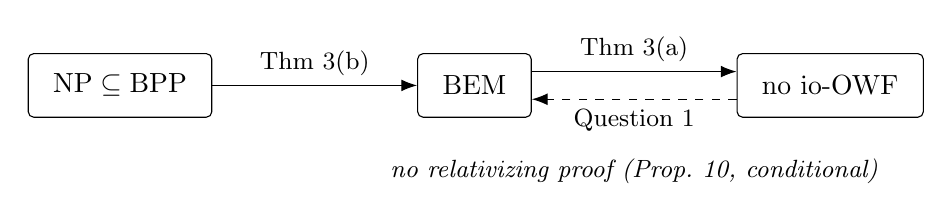
\begin{tikzpicture}[node distance=1.2cm and 2.6cm,
    box/.style={draw, rounded corners=2pt, minimum height=2.3em, inner xsep=9pt, inner ysep=4pt},
    lab/.style={font=\small}]
  \node[box] (a) {$\mathrm{NP} \subseteq \mathrm{BPP}$};
  \node[box, right=of a] (b) {$\mathrm{BEM}$};
  \node[box, right=of b] (c) {no io-OWF};
  \draw[-{Latex[length=2mm]}] (a) -- node[lab, above] {Thm 3(b)} (b);
  \draw[-{Latex[length=2mm]}] ([yshift=5pt]b.east) -- node[lab, above] {Thm 3(a)} ([yshift=5pt]c.west);
  \draw[-{Latex[length=2mm]}, dashed] ([yshift=-5pt]c.west) -- node[lab, below] {Question 1} ([yshift=-5pt]b.east);
  \path (b.south east) -- (c.south west) node[midway, below=0.4cm, lab, font=\small\itshape] {no relativizing proof (Prop.~10, conditional)};
\end{tikzpicture}
\caption{The same-time sandwich, Theorem 3($c$). Question 1 asks whether the second arrow reverses. \emph{Plain reading: easy $\mathrm{NP}$ tames the averages, which forbids one-way functions; the way back is open.}}
\end{figure}

\textbf{What a proof would have to use.} This is a speculation: an unpublished construction of the authors, not reproduced here and conditional on an injective one-way function that is exponentially secure, suggests a polynomial-time samplable pair distribution that violates $\mathrm{BEM}$ although its own function is not even weakly one-way. If that construction is right, no argument that derives $\mathrm{BEM}$ for a distribution $D$ from the non-one-wayness of $D$'s own function alone can prove the converse of Theorem 3, and a proof would have to use the global hypothesis, the non-one-wayness of functions other than the sampler's own. This is recorded as a guess about proof structure; it proves nothing.

\emph{Plain reading: a guess, not a result: if a certain construction holds up, a proof that ``nothing is one-way'' forces tame averages would have to use the easiness of other functions, not only of the one that made the process.}

\begin{definitionx}{9}[{the time-skewed defect and its moment condition}] For a polynomial $P$ with $P(s) \ge s$ and a time bound $s$,
\[
\begin{gathered}
\Sigma^{+}_{s,P}(x, y) := \bigl[\, \mathrm{pK}^{P(s)}(y) + \mathrm{pK}^{P(s)}(x \mid y) \,\bigr] - \bigl[\, \mathrm{pK}^s(x) + \mathrm{pK}^s(y \mid x) \,\bigr], \\
\Sigma^{-}_{s,P}(x, y) := \bigl[\, \mathrm{pK}^{P(s)}(x) + \mathrm{pK}^{P(s)}(y \mid x) \,\bigr] - \bigl[\, \mathrm{pK}^s(y) + \mathrm{pK}^s(x \mid y) \,\bigr].
\end{gathered}
\]

\emph{Plain reading: the same comparison of the two orders of description as $\sigma$, except that the order being bounded above is given polynomially more time, giving two objects, one per direction, with $\Sigma^{-}(x, y) = \Sigma^{+}(y, x)$ and no antisymmetry.}

\end{definitionx}

\textbf{$\mathrm{BEM}_{\mathrm{skew}}$} is the statement: for every polynomial-time samplable pair distribution $D$ there are polynomials $P$, $p_0$ and a constant $C$ such that for all $s \ge p_0(n) \ge n$ and all large $n$, $\mathrm{E}_D[2^{\Sigma^{+}_{s,P}}] \le s^C$ and $\mathrm{E}_D[2^{\Sigma^{-}_{s,P}}] \le s^C$. \emph{Plain reading: some polynomial amount of extra time for the side being compressed makes both exponential averages polynomial in the time budget.} The extra time $P$ is chosen per distribution; the statement carries no hypothesis. The bound is a power of $s$ and not of $n$ because the time loss in the symmetry-of-information input to Proposition 7(a) grows with $s$, so no single power of $n$ works for every $s$; for polynomial $s$ the two readings agree, and that is the only case Proposition 7($c$) uses.

\textbf{The refined sandwich.} With $\mathrm{DistNP} \subseteq \mathrm{AvgBPP}$ the statement that every distributional $\mathrm{NP}$ problem has an errorless randomized heuristic scheme (one randomized polynomial-time algorithm that, given an instance and a failure bound $\varepsilon$, answers ``I don't know'' on at most an $\varepsilon$ fraction of the instances and otherwise answers correctly, up to a small error probability over its own coins on every instance; this is the hypothesis of GKLO22's Lemma 26), Proposition 7 and Theorem 3 give
\[
\begin{gathered}
\mathrm{NP} \subseteq \mathrm{BPP} \;\;\Rightarrow\;\; \mathrm{DistNP} \subseteq \mathrm{AvgBPP} \;\;\Rightarrow\;\; \mathrm{BEM}_{\mathrm{skew}} \;\;\Rightarrow\;\; \text{no io-OWF}, \\
\mathrm{NP} \subseteq \mathrm{BPP} \;\;\Rightarrow\;\; \mathrm{BEM} \;\;\Rightarrow\;\; \mathrm{BEM}_{\mathrm{skew}}
\end{gathered}
\]

\emph{Plain reading: the same-time condition sits between ``$\mathrm{NP}$ is easy'' and the skewed condition; the skewed condition sits between ``$\mathrm{NP}$ is easy on average without errors'' and ``no one-way functions''.}

The first arrow of the left chain is standard and relativizes (an errorless heuristic for a problem that is easy in the worst case is the worst-case algorithm itself). Question 1 asks whether the last arrow of the left chain reverses for the same-time object, that is, whether ``no io-OWF'' reaches all the way back to $\mathrm{BEM}$.

\subsection*{8.2 Remark: the time-skewed variant}
\phantomsection\addcontentsline{toc}{subsection}{8.2 Remark: the time-skewed variant}

\begin{propositionx}{7}[{the skewed sandwich}]

(a) If $\mathrm{DistNP} \subseteq \mathrm{AvgBPP}$ then $\mathrm{BEM}_{\mathrm{skew}}$ holds, and pointwise: there are polynomials $p$, $p_0$ such that with $P(s) := p(c's)$, where $c' \ge c$ is a constant depending only on $U$ ($c$ from Lemma 11, enlarged to cover the $O$($n$)-time re-encoding that prints the pair in the other order, absorbed since $s \ge n$), for all $s \ge p_0(n)$, all large $n$ and every pair $x, y \in \{0,1\}^n$, $\Sigma^{+}_{s,P}(x, y) \le O(\log s)$ and $\Sigma^{-}_{s,P}(x, y) \le O(\log s)$.

(b) $\mathrm{BEM} \Rightarrow \mathrm{BEM}_{\mathrm{skew}}$.

(c) $\mathrm{BEM}_{\mathrm{skew}} \Rightarrow \text{no io-OWF}$.

\emph{Plain reading: (a) if $\mathrm{NP}$ is easy on average without errors, the skewed defect is small on every pair, not only on average; (b) the skewed condition is weaker than the same-time one; (c) the skewed condition still rules out one-way functions.}

\end{propositionx}

\textbf{Proof.} From [GKLO22, Lemma 26(1) together with the sentence following its two items, p. 16:22] and Lemma 11. (a) GKLO22's Lemma 26(1), in the special case without a conditioning string that the source states in the sentence following the lemma, gives: if $\mathrm{DistNP} \subseteq \mathrm{AvgBPP}$ there are polynomials $p$, $p_0$ such that for all large $n$, all $t \ge p_0(n)$ and every $x, y \in \{0,1\}^n$,
\[
\mathrm{pK}^t(x, y) \ge \mathrm{pK}^{p(t)}(x) + \mathrm{pK}^{p(t)}(y \mid x) - \log p(t). \qquad \text{(H1)}
\]

\emph{Plain reading: if $\mathrm{NP}$ is easy on average without errors, then the pair never costs less than $x$ plus $y$-given-$x$, once the parts are allowed polynomially more time.}

Applied to the pair written in the other order it gives (H2), the same inequality with $x$ and $y$ exchanged; the $O(1)$-bit, $O(n)$-time re-encoding puts the reverse-order parts at time $p(cs + O(n))$ rather than $p(cs)$, which only lowers $\Sigma^{+}$ by Lemma 4, so it is absorbed by enlarging $P$. Lemma 11 at time $s$ (it needs $s \ge n$, which $p_0 \ge n$ ensures) gives
\[
\begin{gathered}
\mathrm{pK}^{cs}(x, y) \le \mathrm{pK}^s(x) + \mathrm{pK}^s(y \mid x) + O(\log s) \quad \text{(E1)}, \\
\mathrm{pK}^{cs}(x, y) \le \mathrm{pK}^s(y) + \mathrm{pK}^s(x \mid y) + O(\log s) \quad \text{(E2)}.
\end{gathered}
\]

\emph{Plain reading: the pair costs at most either two-step description, at a constant multiple of the time.}

For $s \ge p_0(n)$ put $t = cs \ge p_0(n)$ in (H1) and (H2). Then (H2) followed by (E1) reads $\mathrm{pK}^{p(cs)}(y) + \mathrm{pK}^{p(cs)}(x \mid y) - \log p(cs) \le \mathrm{pK}^{cs}(x, y) \le \mathrm{pK}^s(x) + \mathrm{pK}^s(y \mid x) + O(\log s)$, which is $\Sigma^{+}_{s,P} \le O(\log s)$; and (H1) followed by (E2) is $\Sigma^{-}_{s,P} \le O(\log s)$. Both hold for every pair, so both exponential averages are at most $2^{O(\log s)} = s^{O(1)}$ under every distribution on pairs, samplable or not, which is the bound Definition 9 asks for.

(b) By Lemma 4, $\mathrm{pK}^{P(s)} \le \mathrm{pK}^s$ term by term for every polynomial $P \ge \mathrm{id}$, so $\Sigma^{+}_{s,P} \le \sigma_s$ and $\Sigma^{-}_{s,P} \le -\sigma_s$ pointwise; the skewed moments are dominated by the same-time ones, whichever $P$ is chosen, and Definition 7's bound $n^C$ is at most Definition 9's $s^C$ because $s \ge n$.

(c) The argument of Theorem 3(a) survives the skew. Let $f$ be an io-OWF and $D = (z, f(z))$. Suppose $\mathrm{BEM}_{\mathrm{skew}}$ held for $D$ with $P$, $p_0$, $C$, and put $s := \max(p_0, t_D)$. The forward-order bracket at time $s$ is $\mathrm{pK}^s(z) + \mathrm{pK}^s(f(z) \mid z) \le n + d + c_f \log n$, as in the proof of Theorem 3(a). At the long time $P(s)$, which is still a polynomial, Lemma 9 with $q$ = 4 gives $\mathrm{pK}^{P(s)}(z \mid f(z)) > \log |f^{-1}(f(z))| + c \log n$ with probability at least $3/4$ for infinitely many $n$, for every constant $c$, and Lemma 7 gives $\mathrm{pK}^{P(s)}(f(z)) \ge \log 1/D_2(f(z)) - 2 - L$ with probability above $3/4$. Since $D_2(f(z)) = |f^{-1}(f(z))| 2^{-n}$, the two lower bounds add to $n + c \log n - 2 - L$. So with probability at least $1/2$, infinitely often,
\[
\Sigma^{+}_{s,P}(z, f(z)) \ge \bigl[\, n + c \log n - \log n - 4 \,\bigr] - \bigl[\, n + d + c_f \log n \,\bigr] = (c - c_f - 1) \log n - d - 4,
\]

\emph{Plain reading: on half the inputs the skewed defect is about $c \log n$, for any $c$ we choose, no matter how much extra time the reverse order is given.}

and, with $k$ such that $s \le n^k$, $\mathrm{E}_D[2^{\Sigma^{+}_{s,P}}] \ge n^{kC+1}$ for infinitely many $n$ once $c$ = kC + $c_f$ + 3, contradicting the bound $s^C \le n^{kC}$.\qed

Why the same-time object does not get the lower top. (H1) has the pair at time $t$ and the parts at the longer time $p(t)$. Moving the reverse-order bracket from time $t$ to time $p(t)$ pushes it down (Lemma 4), so the pointwise bound lands on $\Sigma^{+} \le \sigma$, the wrong side to control $\sigma$ itself. We expect, but do not prove, that every symmetry-of-information statement cited in \S{}8.6 carries a time loss of this kind, except HILNO's, whose same-time form is special to their coding-theorem route and gives only the average-case, $1 - 1/\mathrm{poly}$ level. Whether $\mathrm{DistNP} \subseteq \mathrm{AvgBPP}$ implies same-time $\mathrm{BEM}$ is therefore open; it would need worst-case symmetry of information for $\mathrm{pK}^t$ with no time loss.

\begin{definitionx}{10}[{$\mathrm{H}_{\mathrm{pK}}$, errorless easiness of log-gap compressibility on uniform inputs}] Let $L$ be the language defined in GKLO22's proof of Lemma 26(1), and $D$ the ensemble of that proof, uniform on $(u, v, w, w')$ with the four lengths and $s$ as its index [GKLO22, Lemma 6 and the proof of Lemma 26(1), pp. 16:22--16:24]. $\mathrm{H}_{\mathrm{pK}}$ is the statement $(L, D) \in \mathrm{AvgBPP}$, in the errorless sense of \S{}8.1, the sense in which that proof feeds $(L, D)$ to their Lemma 6. The language is
\[
\begin{gathered}
L = \bigl\{\, (u, v, w, w', 1^s) : \exists\, M \in \{0,1\}^s \text{ such that } M(w, w') \text{ prints } uv \text{ in } |w| \text{ steps,} \\
\text{and } s = |u| + |v| - 10 \,\bigr\}.
\end{gathered}
\]

\emph{Plain reading: $\mathrm{H}_{\mathrm{pK}}$ says that some fast randomized algorithm, given a random pair of strings and random helper strings, tells whether the pair has a program exactly ten bits shorter than itself that prints it, given the helpers, within as many steps as the first helper is long; it is right on most inputs, may say ``I don't know'', and lies only with small probability over its own coins.}

\end{definitionx}

\begin{propositionx}{8}[{the top of the skewed sandwich, lowered}] Assume, as read, that the proof of [GKLO22, Lemma 26(1)] uses $\mathrm{DistNP} \subseteq \mathrm{AvgBPP}$ only once, to obtain the Lemma-6 algorithm for $(L, D)$ [GKLO22, Lemma 6 and the proof of Lemma 26(1), pp. 16:22--16:24]. Then:

(a) $\mathrm{H}_{\mathrm{pK}}$ implies symmetry of information for $\mathrm{pK}^t$ in the form of GKLO22's Lemma 26(1), in the special case with no conditioning string, stated by the source in the sentence following Lemma 26: there are polynomials $p$, $p_0$ such that (H1) of the proof of Proposition 7 holds for all large $n$, all $t \ge p_0(n)$ and every $x, y \in \{0,1\}^n$.

(b) Hence $\mathrm{H}_{\mathrm{pK}} \Rightarrow \mathrm{BEM}_{\mathrm{skew}}$, pointwise and with the bounds of Proposition 7(a), by the proof of Proposition 7(a) unchanged.

(c) $\mathrm{DistNP} \subseteq \mathrm{AvgBPP} \Rightarrow \mathrm{H}_{\mathrm{pK}}$, since $L \in \mathrm{NP}$ and $D$ is samplable; so (b) weakens the hypothesis of Proposition 7(a).

\emph{Plain reading: to make the skewed defect small on every pair, you do not need all of $\mathrm{NP}$ to be easy on average without errors; you need one specific counting problem about description length to be easy on average without errors.}

\end{propositionx}

\textbf{Proof.} (a) is GKLO22's proof of Lemma 26(1) with its one sentence ``Using the assumption that $\mathrm{DistNP} \subseteq \mathrm{AvgBPP}$, it follows that $(L, D) \in \mathrm{AvgBPP}$'' [GKLO22, p. 16:23] replaced by the hypothesis $\mathrm{H}_{\mathrm{pK}}$; no other line of that proof uses the hypothesis, what follows being a counting argument, a hybrid argument and an appeal to their Lemma 22. (b) is the derivation in the proof of Proposition 7(a), which consumes only the Lemma-26 inequality (H1) and its mirror (H2). (c) is the definition of $\mathrm{DistNP} \subseteq \mathrm{AvgBPP}$: $L \in \mathrm{NP}$ is noted in the same proof, and $D$ is samplable.\qed

\begin{propositionx}{9}[{no relativizing argument collapses the skewed sandwich to $\mathrm{NP} \subseteq \mathrm{BPP}$}] Assume (i) the oracle of [Hirahara and Nanashima 2021, Theorem 3 (ECCC TR21-161, \S{}6)]: an oracle $O$ with
\[
\mathrm{DistPH}^O \subseteq \mathrm{AvgP}^O \qquad \text{and} \qquad \mathrm{UP}^O \cap \mathrm{coUP}^O \not\subseteq \mathrm{BPTIME}^O\bigl[\, 2^{n / \omega(\log n)} \,\bigr];
\]

\emph{Plain reading: relative to $O$, every distributional problem in the polynomial hierarchy has an errorless fast heuristic, yet some problem with unique witnesses on both sides has no fast randomized algorithm, even one allowed almost exponential time.}

and (ii) GKLO22's remark after their Definition 17 that all the results of their Section 3 also hold with any oracle [GKLO22, \S{}3, p. 16:18], which covers Lemma 26 (their \S{}3.4). Then no relativizing argument proves $\mathrm{BEM}_{\mathrm{skew}} \Rightarrow \mathrm{NP} \subseteq \mathrm{BPP}$.

\end{propositionx}

\textbf{Proof.} Relative to $O$: $\mathrm{DistNP}^O \subseteq \mathrm{AvgBPP}^O$, so Proposition 7(a) relativized gives $\mathrm{BEM}_{\mathrm{skew}}^O$; and $\mathrm{NP}^O \not\subseteq \mathrm{BPP}^O$, since $\mathrm{UP} \cap \mathrm{coUP} \subseteq \mathrm{NP}$. Hence ``$\mathrm{BEM}_{\mathrm{skew}} \Rightarrow \mathrm{NP} \subseteq \mathrm{BPP}$'' is false relative to $O$, and no argument that relativizes collapses the skewed sandwich to its top. (By Proposition 7($c$) relativized there are also no io-OWF relative to $O$: it is a world with $\mathrm{NP}$ hard and nothing one-way.)\qed

Proposition 9 concerns the skewed top arrow only. What is known about the two arrows of the same-time sandwich relative to oracles is in \S{}8.3.

\subsection*{8.3 Oracle evidence for the same-time sandwich}
\phantomsection\addcontentsline{toc}{subsection}{8.3 Oracle evidence for the same-time sandwich}

Everything in this subsection is relative to an oracle $O$: $\mathrm{pK}^t$ is computed by a universal machine with oracle access, samplers and inverters may query $O$, and every class carries the superscript $O$. GKLO22 state that their results hold in this setting [GKLO22, \S{}1.2, and the remark after Definition 17, \S{}3, p. 16:18], and \S{}8.7 records that every object of this paper relativizes. Two average-case classes are needed beyond those of \S{}8.1. $\mathrm{DistNP} \subseteq \mathrm{HeurP}$ is error-prone easiness: every distributional $\mathrm{NP}$ problem has one polynomial-time algorithm that, given an instance and an error bound $\varepsilon$, is wrong on at most an $\varepsilon$ fraction of the instances at each length (an error-prone heuristic scheme) [Hirahara and Nanashima 2022, \S{}3.1]; the $\mathrm{P}$ of $\mathrm{HeurP}$ makes the algorithm deterministic, and ``polynomial time'' means polynomial in the instance length and $1/\varepsilon$, the convention Hirahara and Nanashima take from [Impagliazzo 1995, Proposition 3]. $\mathrm{HeurBPP}$ is the randomized form of the same scheme, with the error bound given in unary, so $\mathrm{HeurP} \subseteq \mathrm{HeurBPP}$ [HILNO, pp. 17--18]. $\mathrm{DistNP} \subseteq \mathrm{AvgP}$ is the errorless counterpart, where the algorithm may answer ``I don't know'' on that fraction but never lies; \S{}8.1's $\mathrm{DistNP} \subseteq \mathrm{AvgBPP}$ is its randomized form.

\textbf{The bottom arrow.} The world is the error-prone Heuristica of Hirahara and Nanashima, named after the Heuristica of Impagliazzo's five worlds [Impagliazzo 1995]. Their Theorem 4 [Hirahara and Nanashima 2022, \S{}1.1] gives, for every constant $a > 0$, an oracle $O$ relative to which, among other things,
\[
\mathrm{DistNP}^O \subseteq \mathrm{HeurP}^O \qquad \text{and} \qquad \mathrm{DistNP}^O \not\subseteq \mathrm{AvgSIZE}^O\bigl[\, 2^{a n / \log n} \,\bigr];
\]

\emph{Plain reading: relative to $O$, every distributional $\mathrm{NP}$ problem is easy on average if the algorithm may lie on a rare fraction of inputs, and some distributional $\mathrm{NP}$ problem is hard on average, even for circuits of nearly exponential size, if the algorithm must never lie.}

the same theorem lists an auxiliary-input one-way function against circuits of that size. The oracle is drawn at random; Theorem 15 [Hirahara and Nanashima 2022, \S{}5] states that the first inclusion holds with probability 1 over the draw.

The construction [Hirahara and Nanashima 2022, \S{}4], in the terms needed here. $O_a = F + A$. $F$ is a table of random bits $F(z, x, \ell)$ for $z, x \in \{0,1\}^n$ and $\ell \in [n]$; write $R_z(x) := F(z, x, 1) \cdots F(z, x, n)$ for the row of $(z, x)$. The table is revealed in levels $i = 1, \dots, i_{\max}(n)$: at level $i$ a random restriction assigns each still-open bit a uniform value with probability $1 - p(n)$ and keeps it open with probability $p(n)$, and a random set $S_{n,i}$ of the $z$'s, of size $p(n) \cdot |S_{n,i-1}|$, has its whole rows kept open regardless (the masks); at the last level everything still open is assigned uniformly. The parameters are $p(n) = 2^{-6an/\log n}$ and $i_{\max}(n) = (1/7a) \cdot \log(an/\log n)$. $F$ returns the final value of every bit, masked or not. $A$ answers $\mathrm{NP}$ questions about $F$: on $(M, x, 1^{T^{2c}})$, with $c = 7a$, it builds the $T$-DNF of $M$'s accepting computations, restricts it by the assignments of levels $\le i_T := (1/c) \log \log T$, returns the constant if the restricted formula is constant, and returns 0 otherwise. Proposition 14 [Hirahara and Nanashima 2022, \S{}4]: the answer depends only on the restrictions of levels $\le i_T$ at lengths $\le T$. So $A$ lies on the questions its visible part does not settle; that is what makes the world error-prone.

Fix a polynomial $t$. A program running $t$ steps can only write $A$-queries of length $\le t$, so it reaches levels $i \le i(t) := \max\{ i_T : T^{2c} \le t \} \le (1/c) \log \log t$. For polynomial $t$ and large $n$, $i(t) < i_{\max}(n)$, since $\log \log t$ grows like $\log \log n$ and $\log(an/\log n)$ like $\log n$; so $S_{n,i(t)}$ is a mask level, not the final assignment. Put $M_t := S_{n,i(t)}$, the rows masked at the deepest reachable level, and $\mu := |M_t| / 2^n = p(n)^{i(t)}$. For $t = m^k$, with $m = 2n$ the length of the sampler's strings below,
\[
\log(1/\mu) = 6\, a\, n\, i(t) / \log n \le (6/7) \cdot n \cdot (\log \log m + \log k) / \log n = o(n).
\]

\emph{Plain reading: the masked rows are a rare slice of all rows, but only mildly rare: their rarity is two to the minus something smaller than any constant fraction of $n$.}

Fact $M$, read from the construction: conditioned on the restrictions of all levels $\le i(t)$ at every length, the bits of the masked rows $\{F(z, x, \ell) : z \in M_t\}$ are independent uniform bits, every $A$-answer a time-$t$ program can reach is already fixed, and $F$ returns the true masked bits when queried.

\begin{propositionx}{10}[{the bottom arrow does not reverse by any relativizing argument}] Assume (i)--(iii), where hypothesis (iii) is itself inferred from the construction as read, not proved: (i) the construction of $O_a$ and Fact $M$ as read [Hirahara and Nanashima 2022, \S{}4]; (ii) Theorem 15 as read [Hirahara and Nanashima 2022, \S{}5]; (iii) HILNO's Lemma 33 and Proposition 38 [HILNO, Lemma 33, \S{}5.1, p. 37, and Proposition 38, \S{}5.2, p. 42], taken to relativize, the reason for the inference being that Lemma 33 is the search-to-decision reduction of Ben-David, Chor, Goldreich and Luby [1992] with pairwise-independent hashing, giving conditional extrapolation from $\mathrm{DistNP} \subseteq \mathrm{HeurBPP}$, and Proposition 38 runs the extrapolator on $f$($x$) to invert $f$; both are black-box in the oracle. Part (a) uses (i) only. Let $m = 2n$ and let $D$ be the sampler that draws $z, w \in \{0,1\}^n$ uniformly and outputs $(x, y) := ((z, w), R_z(w) 0^n)$, a pair of $m$-bit strings, with $n$ oracle queries; at odd lengths it outputs $(0^m, 0^m)$. Then:

(a) For every polynomial $t \ge t_D$ and every large $n$, with probability at least $1/3$ over the choice of $O_a$,
\[
\mathrm{E}_{D_m} \bigl[\, 2^{+\sigma_t} \,\bigr] \ge \mu^2 \cdot 2^n / \bigl( 2^{O(1)} \cdot t \bigr) = 2^{n - o(n)}.
\]

\emph{Plain reading: on the masked rows, a slice of the sampler's pairs of rarity $\mu$, the ``row first, then pair from row'' description costs about $n$ more bits than the ``pair first, then row from pair'' description, and $n$ is far more than the log of one over $\mu$ that the rarity could pay for; so the exponential average is essentially two to the $n$.}

(b) There is a set of oracles of measure at least $1/3$ relative to each of which $\mathrm{BEM}$ fails, for every polynomial $p_D$ and every constant $C$, and there are no io-OWF. Hence no relativizing argument proves the sharper ``$\mathrm{DistNP} \subseteq \mathrm{HeurP} \Rightarrow \mathrm{BEM}$'' (this clause uses (i) and (ii) only), and, with (iii), none proves ``$\text{no io-OWF} \Rightarrow \mathrm{BEM}$''.

\end{propositionx}

\textbf{Proof.} (a) Fix a polynomial $t \ge t_D$ (so $t$ covers the $n$ oracle queries of the sampler, which is also what the constant-size program of the forward bracket runs) and condition on the restrictions of levels $\le i(t)$ at every length; this fixes $M_t$ and every reachable $A$-answer, and by Fact $M$ leaves the masked rows uniform. Let $P := M_t \times \{0,1\}^n$ and $N := |P| = \mu 2^{2n}$. Programs in the proof (Appendix B.1) run in time $t$ with oracle $O$ and read the shared random string $r$ of Definition 1. By Definition 1, $\mathrm{pK}^t(y) \le k$ means $\Pr_r[\, \text{some program of length} \le k \text{ prints } y \,] \ge 2/3$, so, by the union bound over programs, a pair with $\mathrm{pK}^t(y) \le k$ has $\sum_{|Q| \le k} \Pr_r[Q \text{ prints } y] \ge 2/3$; the same for $\mathrm{pK}^t(x \mid y)$. The two steps bound the expected number of such pairs by Markov's inequality applied to that sum. Full proof in Appendix B.1.

Four remarks. (1) What breaks $\mathrm{BEM}$ is the masks: whole rows hidden at every reachable level, with rarity $2^{-o(n)}$, far thicker than the $2^{-n/2}$ that the errorless constructions of Proposition 11 allow. The excess on the slice is about $n$ bits and the rarity pays for only $o(n)$ of them. This is the shape \S{}8.4 leaves open, a slice of small mass carrying superpolynomial weight, the shape Proposition 12 below (\S{}8.4) said the hard mass would have to take. (2) By Lemma 10(ii) the sampler with its outputs exchanged breaks $\mathrm{E}[2^{-\sigma_t}]$. (3) The $1/3$ is an artefact of Markov's inequality. Concentration over the independent masked bits would give probability $1 - 2^{-\Omega(N)}$ for each fixed $(n, t)$; Borel--Cantelli over $n$ would then give measure 1 for each $t$, removing the first Fatou step, and a countable intersection over $t$ the second. This step is not carried out here; we expect it to go through as stated. (4) The statement is not in the literature; the oracle is. Hirahara and Nanashima list hardness of GapMINKT and of GapMCSP, hardness of learning in two forms, and hitting-set generators, auxiliary-input one-way functions, auxiliary-input pseudorandom generators and auxiliary-input pseudorandom functions as consequences of their oracle [Hirahara and Nanashima 2022, Theorem 4], not moments of a symmetry-of-information defect.

\textbf{The same-time top arrow.} Relative to the errorless oracle of Proposition 9, $\mathrm{BEM}_{\mathrm{skew}}^O$ holds and $\mathrm{NP}^O \not\subseteq \mathrm{BPP}^O$. Whether same-time $\mathrm{BEM}^O$ holds there is open. Two facts bound what a proof could look like. First, pointwise conditional coding fails relative to that oracle: the converse direction of HILNO's Theorem 4 relativizes (by the argument of \S{}8.7, not carried out here), and $\mathrm{NP}^O \not\subseteq \mathrm{BPP}^O$; so a proof of $\mathrm{BEM}^O$ cannot run through every support pair as Theorem 3(b) does, and must run through averages. Second, the route of Proposition 7(a) yields the skewed object only, for the reason given at the end of \S{}8.2. What has been checked is the natural test.

\begin{propositionx}{11}[{informal; the natural test distributions in two errorless worlds; a remark, not a barrier}] Inferred from the constructions as read, not proved: [Hirahara and Nanashima 2021, \S{}6.1] and Impagliazzo's oracle [Impagliazzo 2011]. Relative to the Hirahara--Nanashima 2021 oracle of Proposition 9, and relative to Impagliazzo's 2011 oracle ($\mathrm{DistNP}^O \subseteq \mathrm{AvgP}^O$ with $\mathrm{NP}^O$ hard, built from a random permutation of $\{0,1\}^n$ revealed in stages, each stage assigning, as Hirahara and Nanashima describe the constraint, all but at most the square root of the number of entries still unassigned, and a restricted $\mathrm{NP}$ oracle), the natural test distributions have bounded exponential moments: the samplers that output ($x$, hidden value at $x$) where their level determines the value, and $\bot$ or a guessed value where it does not. This is a statement about those samplers, not about every sampler; the general case is the open question below. In the 2021 world the check is trivial, since the natural sampler can print a hidden symbol only by guessing it; the parameter count below is non-trivial only for a direct-evaluation variant of that oracle, which is not Hirahara and Nanashima's oracle; and the Impagliazzo half rests on Hirahara and Nanashima's description of that oracle, the original not having been opened. The reason is a parameter count. On the hidden slice $S$ of such a sampler's pairs, the defect is, on exponential average over the slice, at most the number of hidden bits per pair plus $O(\log n)$, and both constructions force that number to be at most $\log(1/D(S))$, so
\[
\mathrm{E}_D \bigl[\, 2^{+\sigma_t} \cdot \mathbf{1}_S \,\bigr] = D(S) \cdot \mathrm{E}_D \bigl[\, 2^{\sigma_t} \bigm| S \,\bigr] \le D(S) \cdot 2^{\log(1/D(S)) + O(\log n)} = n^{O(1)}.
\]

\emph{Plain reading: the hidden slice has mass $D(S)$, and two to the defect, averaged over the slice, is at most one over that mass times a polynomial, so the slice contributes at most a polynomial to the exponential average; the thinness of the slice pays for the hidden bits.}

\end{propositionx}

The argument continues in Appendix B.2.

Contrast with Proposition 10: there the hidden rows carry about $n$ bits each while the slice's rarity is $2^{-o(n)}$, so the thinness does not pay, and the exponential average is $2^{n - o(n)}$.

\textbf{Status of the top arrow.} The relativization test for the same-time top arrow has therefore been run on the natural distributions of both errorless worlds, where the moments are bounded, trivially in one world and by a parameter count on a variant of the oracle in the other; the general case, same-time $\mathrm{BEM}$ relative to the Hirahara--Nanashima 2021 oracle, is open. The obstacle an unpublished note of the authors identifies for the general case is a rare-slice step in the sense of \S{}8.4, bounding the excess of the defect on the slice where an errorless heuristic answers ``I don't know'', and not a time-skew step. Nothing further is attempted here; the question is sharpened in \S{}8.5.

\textbf{The skewed object in the error-prone world.} Inferred from the proof of Proposition 10 as written, not proved: relative to the oracles of Proposition 10(b), $\mathrm{BEM}_{\mathrm{skew}}$ fails as well, and with it $\mathrm{H}_{\mathrm{pK}}$. The proof of (a) (Appendix B.1) fixes a polynomial $t$, lower-bounds $\mathrm{pK}^t(y)$ and $\mathrm{pK}^t(x \mid y)$ on the masked slice $M_t$, and compares them with a forward bracket of $2n + O(1)$ at the same time. In $\Sigma^{+}_{s,P}$ the two lower-bounded terms sit at the longer time $P(s)$ and the forward bracket at time $s$. $P$ is a polynomial, so $i(P(s)) \le (1/c) \log \log P(s) = O(\log \log n)$ is still a mask level, the display for $\log(1/\mu)$ gives $o(n)$ with $M_{P(s)}$ in place of $M_s$, the forward bracket is unchanged, and the two Markov steps run at time $P(s)$ give $\mathrm{E}_{D_m}[2^{\Sigma^{+}_{s,P}}] \ge 2^{n - o(n)}$ with probability at least $1/3$, for every polynomial $P$ and every $s \ge t_D$. Since $\Sigma^{+}_{s,P}$ only falls as $P$ grows (Lemma 4), it is enough to treat $P_j(s) := s^j$; the two Fatou steps of (b) run for each $j$ as before, with the events taken at the common threshold $2^{n/2}$ in place of $2^{n - o(n)}$, so that the oracle sets so obtained are nested in $j$ and their intersection has measure at least $1/3$, and relative to every oracle in it Definition 9 fails for $D$ at every $P$, $p_0$ and $C$. By the contrapositive of Proposition 8(b), which relativizes by the GKLO22 remark cited in Proposition 9, $\mathrm{H}_{\mathrm{pK}}$ also fails there. So in the error-prone world both sides of the converse of Proposition 8(b) are false, and in the two errorless worlds of Proposition 11 both are true ($\mathrm{H}_{\mathrm{pK}}$ by Proposition 8($c$), $\mathrm{BEM}_{\mathrm{skew}}$ by Proposition 9 and by Proposition 7(a) relativized): no oracle on record separates $\mathrm{BEM}_{\mathrm{skew}}$ from $\mathrm{H}_{\mathrm{pK}}$, and what blocks the converse is the quantitative obstruction named in \S{}8.5, not a barrier theorem.

\emph{Plain reading: the oracle world that breaks the same-time bound also breaks the skewed bound, because giving the reverse-order description polynomially more time still leaves it inside the masked levels where the rows are hidden, and there the one counting problem is hard too, so the two sides of the open converse are both false in that world and both true in the two errorless worlds: no known oracle world tells them apart, and what stands in the way of the converse is a matter of size, not a black-box impossibility.}

\subsection*{8.4 The two obstacles, and where the excess lives}
\phantomsection\addcontentsline{toc}{subsection}{8.4 The two obstacles, and where the excess lives}

Two obstacles stand between the sandwich's ends and its middle, one per arrow.

\textbf{At the top $(\mathrm{BEM} \Rightarrow \mathrm{NP} \subseteq \mathrm{BPP})$.} A proof would turn a condition on every samplable distribution into a worst-case algorithm for $\mathrm{NP}$; read contrapositively, it would derive average-case hardness, a $\mathrm{BEM}$ violation, from worst-case hardness of $\mathrm{NP}$. Reductions of that shape that are non-adaptive and black-box, from worst-case $\mathrm{NP}$ to average-case solvers of the $1 - 1/\mathrm{poly}$ kind, are known to collapse the polynomial hierarchy to its third level [Feigenbaum and Fortnow 1993; Bogdanov and Trevisan 2006]. Those results are stated for $1 - 1/\mathrm{poly}$ conditions and not for an exponential-tail condition like $\mathrm{BEM}$, so they do not close the door; they say that a proof must be adaptive or non-black-box, or must use the exponential tail specifically. This is our description of the obstacle, not a theorem; the cited collapse theorems are not used in any proof here.

\textbf{At the bottom $(\text{no io-OWF} \Rightarrow \mathrm{BEM})$.} The quantifiers do not match. ``No io-OWF'' is, by Proposition 1, of the form ``for every accuracy $1/q$ there is a time $p(q)$'': accuracy is bought with time. $\mathrm{BEM}$ is of the form ``there is one time $p_D$, and then the tail $2^{-k}$ holds at every level $k$ up to $n$''. Universal-search arguments make an inverter uniform in time only relative to competitors of smaller time; no principle is known that makes accuracy uniform in this way. This description of the obstacle is likewise ours, not a theorem.

The bottom obstacle has an exact form. Under the hypothesis of Question 1, everything that could make the exponential averages large is confined to a slice of the sampler's pairs of polynomially small mass, and the slice can be made as thin as any polynomial at the price of a time bound that grows with the thinness.

\begin{propositionx}{12}[{where the excess lives without one-way functions}] If io-OWFs do not exist, then for every polynomial-time samplable pair distribution $D$ and every polynomial $q$ there is a polynomial $p$ such that for all $t \ge p(n)$ and all large $n$ there is a set $G = G_q \subseteq \operatorname{supp} D$ (it depends on $q$ and $p$, not on $t$) with $D(G) \ge 1 - 2/q(n)$ and
\[
\mathrm{E}_D \bigl[\, 2^{-\sigma_t} \cdot \mathbf{1}_G \,\bigr] \le n^{O(1)} \qquad \text{and} \qquad \mathrm{E}_D \bigl[\, 2^{+\sigma_t} \cdot \mathbf{1}_G \,\bigr] \le n^{O(1)}.
\]

\emph{Plain reading: without one-way functions, whatever could make the exponential average blow up sits on a slice of the sampler's pairs of mass at most $2/q$, for any polynomial $q$ you name, at the price of a time bound that grows with $q$.}

\end{propositionx}

\textbf{Proof.} Proposition 1(ii) applied to $D$ and to the swapped distribution $(y, x)$ gives a polynomial $p$ such that, for all large $n$, $\mathrm{pK}^p(x \mid y) \le \log 1/D(x \mid y) + \log p$ with probability at least $1 - 1/q$ and $\mathrm{pK}^p(y \mid x) \le \log 1/D(y \mid x) + \log p$ with probability at least $1 - 1/q$; let $G$ be the set of support pairs where both hold, so $D(G) \ge 1 - 2/q$. Take $p \ge t_D$. On $G$ and for $t \ge p$, Lemma 4 and Lemma 5 give, as in the proof of Theorem 3(b), $m_F \ge D(x, y) / (p n^{c_D})$ and $m_R \ge D(x, y) / (p n^{c_D})$. Then
\[
\mathrm{E}_D \bigl[\, 2^{-\sigma_t} \cdot \mathbf{1}_G \,\bigr] = \sum_G D \cdot m_R / m_F \le p\, n^{c_D} \sum_G m_R \le p\, n^{c_D}\, (3/2)^2 (n + d)^2,
\]

\emph{Plain reading: on the good slice, two to minus the defect is at most a polynomial times the reverse weight, and the reverse weights add up to at most about $n$ squared.}

by the Kraft display in the proof of Theorem 1(a); the other sign is the same with $\sum_G m_F$.\qed

Conversely, for any set of mass at least $1 - 2/q$ that carries only polynomial moment, Theorem 3(a) says that if io-OWFs exist the weight outside it is superpolynomial infinitely often. So Question 1 is exactly whether a set of polynomially small mass can carry superpolynomial exponential weight. Note the quantifier order: $G$ and $p$ depend on $q$, whereas $\mathrm{BEM}$ asks for one $p$ and every tail level. The reading from physics is Jarzynski's: exponential averages of work are dominated by rare realizations, and the trajectories that carry them look like typical reverse trajectories run backward [Jarzynski 2006]. Physics has no theorem forcing the rare realizations to carry bounded weight, and for $\sigma_t$ there is no normalization identity to do the work (Remark 4). The reading runs from computation to physics; nothing above rests on it.

\subsection*{8.5 The errorless and error-prone divide}
\phantomsection\addcontentsline{toc}{subsection}{8.5 The errorless and error-prone divide}

There are two ways for $\mathrm{NP}$ to be easy on average, and \S{}8.3 used both. Errorless easiness: the fast algorithm may say ``I don't know'' on rare inputs but never lies ($\mathrm{DistNP} \subseteq \mathrm{AvgP}$; randomized, $\mathrm{AvgBPP}$). Error-prone easiness: it may lie on rare inputs ($\mathrm{DistNP} \subseteq \mathrm{HeurP}$; randomized, $\mathrm{HeurBPP}$). Whether the two coincide for $\mathrm{NP}$ is open; it is the subject of [Hirahara and Santhanam 2022] and of [Hirahara and Nanashima 2022], whose oracle separates them: the two displayed items of their Theorem 4 in \S{}8.3 are the two kinds of easiness pulled apart.

\textbf{The divide.} We expect, but do not prove, that bounded exponential moments behave like an errorless condition, and one-wayness like an error-prone one. The evidence is all in this section. Errorless easiness implies the moment bound in skewed form, Proposition 7(a). Error-prone easiness implies no io-OWF, but does not imply the moment bound by any relativizing argument, Proposition 10. In the two errorless worlds the natural distributions have bounded moments, Proposition 11, an inference; in the error-prone world the natural distribution fails. Put with Proposition 7 and Proposition 10 (the middle arrow is HILNO's Theorem 3 with Proposition 1, as in the proof of Proposition 10):
\[
\begin{gathered}
\mathrm{DistNP} \subseteq \mathrm{AvgBPP} \;\;\Rightarrow\;\; \mathrm{BEM}_{\mathrm{skew}} \;\;\Rightarrow\;\; \text{no io-OWF}, \qquad \mathrm{DistNP} \subseteq \mathrm{HeurP} \;\;\Rightarrow\;\; \text{no io-OWF}, \\
\mathrm{DistNP} \subseteq \mathrm{HeurP} \;\;\nRightarrow_{\mathrm{rel}}\;\; \mathrm{BEM}.
\end{gathered}
\]

\emph{Plain reading: errorless easiness gives the skewed moment bound and so no one-way functions, while error-prone easiness gives no one-way functions but provably not the moment bound by black-box means (the crossed arrow: no proof that works in every oracle world exists), so the moment bound is a condition of the errorless kind and one-wayness is not.}

The heuristic account of why the two kinds of algorithm differ on an exponential average (the confession rate of an errorless algorithm on hidden points) is not argued here; it is deferred to an unpublished note of the authors.

Where this leaves the problem. In the terms of \S{}8.4, everything that can make the moments large sits on a rare slice, Proposition 12. The divide says that an errorless algorithm is made to confess on such a slice and an error-prone one is not, and the world of Proposition 10 is one where the confession is never demanded and the slice carries exponential weight. Question 1 (\S{}8.1) asks for $\mathrm{BEM}$ from ``no io-OWF'', a hypothesis of the error-prone kind; Proposition 10 says that no relativizing argument delivers it. The question that remains is the following, stated and not attacked.

\textbf{Sharpened question (status: open).} Does errorless easiness force the same-time moment bound: does $\mathrm{H}_{\mathrm{pK}}$, the errorless easiness of the one distributional problem of Definition 10, imply $\mathrm{BEM}$, for every polynomial-time samplable pair distribution, by an argument that relativizes?
\[
\mathrm{H}_{\mathrm{pK}} \;\;\Rightarrow ?\;\; \mathrm{BEM} \qquad \text{(the same-time question)}
\]

\emph{Plain reading: if the one counting problem about description length has a fast algorithm that may say ``I don't know'' on rare inputs but never lies, must the two exponential averages of the defect be polynomial for every fast process at one time budget, and must the proof work in every oracle world?}

A ``yes'' would put $\mathrm{BEM}$ between $\mathrm{H}_{\mathrm{pK}}$ and ``no io-OWF'' for the same-time object, where $\mathrm{BEM}_{\mathrm{skew}}$ already sits by Proposition 8 ($\mathrm{DistNP} \subseteq \mathrm{AvgP}$ and $\mathrm{DistNP} \subseteq \mathrm{AvgBPP}$ each imply $\mathrm{H}_{\mathrm{pK}}$, so a yes here is the stronger statement). We expect, but do not prove, that a ``no'' would be an errorless world with hidden rows long relative to their rarity, the opposite of what the two constructions of Proposition 11 provide. Neither is attempted here; Proposition 11 is the evidence on record for the first, Proposition 10 for the divide that makes the question the right one.

\textbf{The characterization question (status: open).} Does the skewed moment bound force a natural property back: does $\mathrm{BEM}_{\mathrm{skew}}$ imply (i), the existence of a $\mathrm{BPP}$-computable natural property for conditional $K^t$ with usefulness $n - O(\log n)$ and largeness $1/2$ in the sense of [Kabanets and Kolokolova 2025, Definition 2.11, \S{}2.3, p. 12], the hypothesis under which Proposition 13 of \S{}8.6 gives $\mathrm{BEM}_{\mathrm{skew}}$?
\[
\mathrm{BEM}_{\mathrm{skew}} \;\;\Rightarrow ?\;\; \text{(i)} \qquad \text{(the characterization question)}
\]

\emph{Plain reading: if the two skewed exponential averages are polynomial for every fast process, must there be a fast test that, given any helper string, says ``random'' to at least half of all strings and never says it to a string with a short program given the helper?}

This is the technical challenge Kabanets and Kolokolova state in their concluding remarks, to derive a polynomial-time natural property from an assumed symmetry of information [Kabanets and Kolokolova 2025, \S{}8], pinned at logarithmic usefulness, since $n - O(\log n)$ is what Proposition 13 consumes. Two obstructions are on record, with different accountings. Obstruction A, the block partition: their Theorem 4.3 turns the chain rule into a natural property by cutting $x$ into $\ell = n/O(\log t)$ blocks and searching one block by brute force; it loses $\Theta(n)$ bits of usefulness even when the chain rule has no error at all, from the per-block union bound and the per-block error, and it needs the chain rule for a super-constant number of strings, which two-string symmetry of information is not known to give in the time-bounded setting [Kabanets and Kolokolova 2025, Theorem 4.3 and its proof, \S{}4.2, p. 24, and footnote 2, p. 2]. No oracle argument attaches to Obstruction A. The loss is structural rather than bookkeeping, for a reason short enough to state: polynomial time forces the blocks to have length $O(\log t)$, so there are $\ell = n/O(\log t)$ of them; a string compressible by only $O(\log n)$ bits then saves $O(\log n)/\ell$ bits, a fraction of a bit, per block, which no block-local test can see against the $O(1)$-bit fluctuation of a random block; and blocks large enough to show the 2 log $\ell$ saving the union bound needs, $O(\log n)$ of them, cost $2^{\Omega(n/\log n)}$ to search, which is the bound of their Appendix B. So the two obstructions are one wall seen from the two ends of the block-size trade-off (an inference; the accounting is in an unpublished note of the authors). Obstruction B, the depth term: their Appendix B derives a natural property from symmetry of information in time $2^{O(n/\log n)}$, the search for a shortest program costing the computational depth of $x$, $O(n/\log n)$ at an instance-dependent superpolynomial time bound [Kabanets and Kolokolova 2025, Appendix B, Theorem B.2 and Lemma B.1], and Hirahara argues informally that a relativizing technique is unlikely to improve the depth term in his own setting, since it would solve every $\mathrm{NP}$ language in time $2^{o(n/\log n)}$ against the Hirahara--Nanashima oracle [Hirahara 2022, Remark 6.4, \S{}6, p. 26:22]; every object of this paper relativizes (\S{}8.7), so, by the analogy of the depth term and not by citation, the natural-property route to the converse with the present machinery is, if that argument is right, closed on quantitative grounds, which we infer but do not prove here.

\emph{Plain reading: the field already asks this question, and the paper asks it at the sharpest setting, a test that misses only a logarithmic number of bits; two things are known to block it: cutting a string into small pieces and testing one piece wastes a fixed fraction of the string, and the one attempt to do better found that a saving of a few bits spread over many pieces cannot be seen in any single piece, while searching for the shortest program instead costs a time that is exponential in $n$ over $\log n$, which Hirahara argues informally a black-box argument is unlikely to beat; if that is right, this route is closed to the black-box methods this paper uses.}

\subsection*{8.6 Placement}
\phantomsection\addcontentsline{toc}{subsection}{8.6 Placement}

We infer, but do not prove, that Question 1 is a form of a recognised one, not a new one. Kabanets and Kolokolova write that symmetry of information for $K^t$ is sandwiched between two average-case assumptions, that every one-way function candidate can be efficiently inverted on average [Longpr\'e and Mocas 1993; Longpr\'e and Watanabe 1995] and that $\mathrm{NP}$ is easy on average [Hirahara 2022, Theorem 1.2; Goldberg and Kabanets 2022], extended to $\mathrm{pK}^t$ under $\mathrm{DistNP} \subseteq \mathrm{AvgBPP}$ by [GKLO22], and that an exact complexity-theoretic characterization of symmetry of information for $K^t$ is missing [Kabanets and Kolokolova 2025, \S{}1.3]. Their concluding remarks ask, as an open question, what complexity assumption would be equivalent to the worst-case symmetry of information, or the chain rule on a constant number of strings, for conditional $K^t$ or $\mathrm{pK}^t$ [Kabanets and Kolokolova 2025, \S{}8]; their own theorem characterizes the worst-case chain rule for conditional $\mathrm{pK}^t$ with multiple strings and sublinear error, $e(N) \le o(N)$ [Kabanets and Kolokolova 2025, Theorem 1.2]. Proposition 8 places the skewed moment bound in that landscape:
\[
\begin{gathered}
\mathrm{DistNP} \subseteq \mathrm{AvgBPP} \;\;\Rightarrow\;\; \mathrm{H}_{\mathrm{pK}} \;\;\Rightarrow\;\; \mathrm{BEM}_{\mathrm{skew}} \;\;\Rightarrow\;\; \text{no io-OWF} \\
\Leftrightarrow\;\; \text{average-case symmetry of information for } \mathrm{pK}^t \text{ at level } 1 - 1/\mathrm{poly} \\
\Rightarrow\;\; \text{error-prone average-case computation of } K \text{ on samplable } D
\end{gathered}
\]

\emph{Plain reading: the moment bound sits between ``description length is computable on average without lying'' and ``description length is computable on average, lying allowed'', which is where Hirahara puts ordinary symmetry of information.}

The arrows, in order: the definition of $\mathrm{DistNP} \subseteq \mathrm{AvgBPP}$, Proposition 8($c$); Proposition 8(b); Proposition 7($c$); [HILNO, Theorem 1, items 1 and 2]; and [HILNO, \S{}1.3, p. 12]. The last arrow is HILNO's exposition of the mechanism behind their Theorem 2: under no one-way function, by Ilango, Ren and Santhanam, for every polynomial-time samplable distribution $D$ there is an efficient average-case algorithm that approximates the resource-unbounded Kolmogorov complexity $K(x)$ of $x \sim D$, an error-prone heuristic; the converse is Ilango, Ren and Santhanam's Theorem 1 [Ilango, Ren and Santhanam 2021, Theorem 1, \S{}1.1], stated there for standard rather than infinitely-often one-way functions, which is why the arrow is drawn one way here. The converse of Proposition 8(b), whether $\mathrm{BEM}_{\mathrm{skew}}$ implies $\mathrm{H}_{\mathrm{pK}}$, is the errorless-versus-error-prone gap for computing $\mathrm{pK}^t$: Hirahara places worst-case symmetry of information for $K^t$ between an errorless and an error-prone heuristic scheme for $K^t$ on samplable inputs, and the two kinds of scheme are known to coincide for problems that admit an instance checker, which $\mathrm{pK}^t$ is not known to admit; Hirahara's placement is under a circuit lower bound for $\mathrm{E}$, which the probabilistic $\mathrm{pK}^t$ does not need here [Hirahara 2022, \S{}1 and Theorem 1.3; Hirahara and Santhanam 2022]. By Lemma 10(iii), $\sigma_t$ is the symmetry-of-information asymmetry for $\mathrm{pK}^t$, so $\mathrm{BEM}$ is the exponential-moment form of average-case symmetry of information with $O(\log n)$ error, and it interpolates the two known levels in tail strength. Hu, Manor and Oliveira prove that symmetry of information fails unconditionally for rKt and for pKt with the time cost charged into the measure [Hu, Manor and Oliveira 2026, \S{}1.2]; those are different measures from the fixed-time $\mathrm{pK}^t$ used here, and their results are cited only with that qualifier.

\begin{propositionx}{13}[{a second top for the skewed sandwich; the Kabanets--Kolokolova chain rule at logarithmic usefulness}] Assume [Kabanets and Kolokolova 2025, Theorem 3.4, \S{}3.3, p. 21] as read, with one clause: their Definition 2.11 asks the property's time parameter to be at least a fixed polynomial in the combined length of the input and the conditioning string, while the proof of Theorem 3.4 calls the property at time $2t$ on a conditioning string of length at least $2t$, which no polynomial allows; calling it at that polynomial of the actual lengths instead leaves the yes-side, the largeness and the polynomial time bounds intact (an inference; the same clause applies to their own Theorem 6.3). Write (i) for the hypothesis: there is a $\mathrm{BPP}$-computable natural property for conditional $K^t$ in the sense of [Kabanets and Kolokolova 2025, Definition 2.11, \S{}2.3, p. 12] with usefulness $n - O(\log n)$ and largeness $1/2$, that is, a randomized polynomial-time predicate $A(x, y, 1^t)$ which, for some polynomial $p$ and all $t \ge p(|x| + |y|)$, accepts with probability at least 0.9 every $x$ with $K^t(x \mid y) \le |x| - O(\log |x|)$, and, for every $y$, rejects with probability at least 0.9 at least half of the strings $x$ of each length.

(a) Under (i) there are constants $c_0, c_1$ such that for all large $n$, every $x, y \in \{0,1\}^n$ and every $t \ge (2n)^{c_0}$,
\[
\mathrm{pK}^t(x, y) \ge \mathrm{pK}^{t^{c_1}}(x) + \mathrm{pK}^{t^{c_1}}(y \mid x) - O(\log n).
\]

\emph{Plain reading: describing the pair costs at least as much as describing the first string and then the second given the first, up to a logarithmic slack, once the two parts are given polynomially more time.}

(b) Hence (H1) and (H2) of the proof of Proposition 7 hold with $p(t) := t^{c_1}$, $p_0(n) := (2n)^{c_0}$ and loss $O(\log n)$ in place of $\log p(t)$, so $\text{(i)} \Rightarrow \mathrm{BEM}_{\mathrm{skew}}$, pointwise and with the bounds of Proposition 7(a), by the proof of Proposition 7(a) unchanged, with the same constant $c'$ in $P$.

\emph{Plain reading: a fast test that says ``no'' to half of all strings whatever the helper string, and says ``yes'', with probability at least 0.9, to every string with a short program given the helper, is enough to make the skewed defect small on every pair, a second way in beside $\mathrm{H}_{\mathrm{pK}}$ that needs no assumption about derandomization.}

\end{propositionx}

\textbf{Proof.} (a) Theorem 3.4 states: if there is a $\mathrm{BPP}$-computable natural property for conditional $K^t$ with usefulness $n - \delta(n, t)$, then there are constants $c_0, c_1$ such that for every $\ell$, all large $x_1, \ldots, x_\ell$ with $N := \sum_i |x_i|$, every $y$ and every $t \ge (N + |y|)^{c_0}$,
\[
\mathrm{pK}^t(x_1, \ldots, x_\ell \mid y) \ge \sum_i \mathrm{pK}^{t^{c_1}}(x_i \mid y, x_1, \ldots, x_{i-1}) - \ell \cdot O(\log N) - \delta(2N, 2t).
\]

\emph{Plain reading: the tuple costs at least the sum of the costs of its parts, each given the earlier parts, minus a slack of one logarithm per part and the test's own shortfall.}

The theorem carries no derandomization hypothesis [Kabanets and Kolokolova 2025, Theorem 3.4 and its proof, \S{}3.3, pp. 21--22]. Its proof is parametric in $\delta$; their own uses of it take $\delta$ linear in $n$. Take $\ell = 2$, $x_1 = x$, $x_2 = y$, the conditioning string empty, so $N = 2n$, and $\delta(n, t) = O(\log n)$: the error is $2 \cdot O(\log 2n) + O(\log 4n) = O(\log n)$, which is the display, up to the re-encoding of the pair absorbed as in the proof of Proposition 7(a). Exchanging the roles of $x$ and $y$ gives (H2). (b) The proof of Proposition 7(a) consumes only (H1), (H2), Lemma 4 and Lemma 11, with a loss $O(\log s)$ at $s \ge n$.\qed

With Proposition 8 the placement now has two tops, not known to be comparable:
\[
\begin{gathered}
\mathrm{DistNP} \subseteq \mathrm{AvgBPP} \;\;\Rightarrow\;\; \mathrm{H}_{\mathrm{pK}} \;\;\Rightarrow\;\; \mathrm{BEM}_{\mathrm{skew}} \;\;\Rightarrow\;\; \text{no io-OWF}, \\
\text{(i)} \;\;\Rightarrow\;\; \mathrm{BEM}_{\mathrm{skew}} \qquad \text{[Proposition 13]}
\end{gathered}
\]

\emph{Plain reading: two different easiness conditions, neither known to imply the other, each force the skewed moment bound: the counting problem being easy on average without lying, and a fast test that calls most strings random given any helper.}

No route from (i) to $\mathrm{H}_{\mathrm{pK}}$ appeared; and the route from $\mathrm{H}_{\mathrm{pK}}$ to (i), the observation that the ``no'' answers of an errorless scheme for $(L, D)$ form a natural property for conditional $K^t$ with usefulness $n - 10$, delivers largeness only on average over the helper strings $(w, w')$, where Definition 2.11 demands it for every conditioning string (an inference; not proved here); GKLO22's own conditional form of Lemma 26(1) likewise controls the conditioning string only for a $9/10$ fraction of the random strings $r$ [GKLO22, Lemma 26(2), p. 16:22]. So (i) and $\mathrm{H}_{\mathrm{pK}}$ are incomparable on the record: two sufficient conditions for $\mathrm{BEM}_{\mathrm{skew}}$, not a chain.

\subsection*{8.7 Barrier filter}
\phantomsection\addcontentsline{toc}{subsection}{8.7 Barrier filter}

Run before any argument on Question 1. Every object in this paper relativizes: $\mathrm{pK}^t$, the universal sampler, the coding theorems, the Kraft sums, and the hashing behind Propositions 1 and 7; GKLO22 state that their results hold in the presence of any oracle, once for their main theorems and once for every result of their Section 3 [GKLO22, \S{}1.2 and the remark after Definition 17, \S{}3, p. 16:18], and nothing here adds a non-relativizing step. So any proof that reverses either arrow of the sandwich by relativizing means must hold in every oracle world, and an oracle world where an arrow fails to reverse rules such a proof out; \S{}8.2 gives one such world for the skewed top arrow and \S{}8.3 treats the same-time sandwich. Natural proofs and algebrization are not triggered: no circuit lower bound is argued anywhere in the paper, a collapse proof in either direction would be an algorithm (an inverter or a coder), not a lower bound, and nothing is arithmetized. The operative barriers are the two of \S{}8.4.

\section*{9. Interpretation}
\phantomsection\addcontentsline{toc}{section}{9. Interpretation}

\textbf{This section is interpretation, not theorem.} It proves nothing, and Theorems 1 to 4 do not depend on any sentence in it. Every statement about a physical system below is a parallel and is named as one. In keeping with the Conventions (\S{}1.3), no sentence here runs from a physical fact to a conclusion about complexity; ``efficiently samplable'' remains the condition of Definition 2, that a sampler runs in polynomial time, and is never read as a property of a physical system. The illustrations used below, mixed milk and the multiplication of two primes, illustrate the frame. The paper's only example of a dissipating process remains the class of Section 4; multiplication belongs to that class only if it is one-way, which is a conjecture.

\subsection*{9.1 Action contains the information}
\phantomsection\addcontentsline{toc}{subsection}{9.1 Action contains the information}

The principle this section rests on is one sentence: \textbf{action contains the information.} A static state hides the way back. What un-hides it is the action: the path, the history, the record of the process that produced the state. Physics uses the word \emph{action} for a quantity attached to a path rather than to a state; that is the sense borrowed here, and this remark is made once and not repeated.

Bennett [1973, p. 525] made the principle exact for computation. Any computer can be made reversible by keeping a record of every step on a history tape. With the record kept, and a copy of the output taken first, the computation can be run backward, blanking the tape and recovering the input, and this costs nothing in principle: such a machine dissipates ``considerably less than $kT$ of energy per logical step''. With the record erased, reversal is no longer free; erasing a bit costs at least $kT \ln 2$ of heat [Landauer 1961, \S{}4: his operation is ``restore to one'' and his figure ``0.6931 $kT$ per restored bit''; ``erasure'' is the word Bennett uses for it, 1973, p. 525]. Keep the record of the computation and uncomputing is free; erase it and reversing costs work.

In this paper's terms the forward description of a pair is the action, and it is short: the sampler's own probability, $\log 1/D(x, y)$ bits. The backward description is what a bounded observer can rebuild of the erased action from the end state: $\mathrm{pK}^t(y) + \mathrm{pK}^t(x \mid y)$ bits, the output first, then the input from the output. Computational entropy production, Definition 5, is the gap between the two:
\[
\sigma^{\mathrm{rev}}_D(x, y) = \bigl[\, \mathrm{pK}^t(y) + \mathrm{pK}^t(x \mid y) \,\bigr] - \log 1/D(x, y).
\]

\emph{Plain reading: the bits the bounded observer's backward story needs beyond the bits the forward story needed, near zero meaning the observer can rebuild the action from the end state and large meaning the action is gone for that observer.}

Theorem 1 says the gap is never much below zero on average, for every fast process. Theorem 2 says that a gap growing faster than any constant multiple of $\log n$ on average, for some fast process, infinitely often, is exactly the existence of one-way functions.

\subsection*{9.2 Lost and hidden}
\phantomsection\addcontentsline{toc}{subsection}{9.2 Lost and hidden}

Two words are used as defined terms from here on. Information about the start is \textbf{lost} when the end state does not determine it: many pasts give the same present, and no observer, bounded or not, can pick one. Information about the start is \textbf{hidden} when the end state does determine it but the bounded observer cannot compute it within its time $t$. Both are ``hidden without the action''. They differ in whether the action can be rebuilt at all.

\begin{itemize}[leftmargin=1.2em,itemsep=3pt,topsep=3pt,parsep=0pt]

\item \textbf{Mixed milk.} A snapshot of milk stirred into coffee records positions only. The velocities are gone; many pasts give the same photo; unmixing from the photo is impossible, not merely hard. With the velocities the laws run backward as cheaply as forward, which is Loschmidt's point [1876]. Physical irreversibility, as seen through the photo, is many-to-one. The information is \emph{lost}.

\end{itemize}

\begin{itemize}[leftmargin=1.2em,itemsep=3pt,topsep=3pt,parsep=0pt]

\item \textbf{A composite number.} A composite $N = pq$ is not a photo with velocities missing. The product determines its factors uniquely; nothing is lost. What was discarded is the \emph{history} of the multiplication, the trace of the carries and partial products. Keep it and uncomputing is free; erase it and reversing costs work [Bennett 1973, p. 525]. Bennett's own remark marks the boundary between the two words: a reversible machine ``must be allowed to save its input -- otherwise it could not be reversible and still carry out computations in which the input was not uniquely determined by the output''. When the map is many-to-one the input itself must be kept or it is lost; when the map is one-to-one only the history need be kept, or the input is hidden. Computational irreversibility is one-to-one but time-bounded: every bit is present, \emph{hidden} behind work.

\end{itemize}

\begin{itemize}[leftmargin=1.2em,itemsep=3pt,topsep=3pt,parsep=0pt]

\item \textbf{A black hole.} The black hole information problem is the largest instance of the second word, and the field has already written it in this section's terms. Hawking radiation looks thermal, so what fell in looks destroyed; unitarity says it cannot be; and the firewall argument of Almheiri, Marolf, Polchinski and Sully sharpens the contradiction with an observer who collects the early radiation, distils the entanglement it carries with a late qubit, and then falls in [Almheiri, Marolf, Polchinski and Sully 2013]. Harlow and Hayden turned the observer's step into a computational task, decoding that entanglement from a description of the circuit that produced the radiation, and proved that if the task can be done in polynomial time for arbitrary circuits then $\mathrm{SZK} \subseteq \mathrm{BQP}$ [Harlow and Hayden 2013]. Aaronson sharpened the hypothesis to the object of this paper: if injective one-way functions secure against quantum computers exist, the decoding task is hard, and the proof is an inverter, since a successful decoder handed $f$($x$) applies two unitaries read off from itself and returns $x$, his eq. (6.3) [Aaronson 2016b, Theorem 6.5.3 and its proof, \S{}6.5.1]; and he records that no converse is known, easy decoding of the generic task not being known to follow even from $\mathrm{P} = \mathrm{PSPACE}$ [Aaronson 2016b, \S{}6.5.2]. In the two words of this section: what fell in is not lost, since the radiation determines it, and it is hidden, behind a computation that is hard whenever one-way functions exist. That is Theorem 4's sentence, that a process has an arrow for the bounded observer exactly when its reverse is hard to sample, said of a quantum system, by other people, and before this paper (the identification of the two sentences is an inference, not proved here; this paper's $\sigma$ is classical and $\mathrm{BPP}$, and nothing here is derived from it). It is quoted as the parallel it is.

\end{itemize}

\begin{itemize}[leftmargin=1.2em,itemsep=3pt,topsep=3pt,parsep=0pt]

\item \textbf{The time bound is the camera.} The bound $t$ in $\mathrm{pK}^t$ is what turns a state into a photo. An observer with unbounded time factors $N$ by brute force, and Theorem 0 says that at unbounded time no pair has a defect beyond $O(\log n)$. A bounded observer sees the product the way the physicist sees the snapshot. Computational entropy production is the gap between the short forward story and the fastest backward story the bounded observer can tell (Definition 5), and Theorem 2 says when that gap is large.

\end{itemize}

\begin{itemize}[leftmargin=1.2em,itemsep=3pt,topsep=3pt,parsep=0pt]

\item \textbf{Where the analogy breaks.} Visiting every state is not the same as being hard to reverse: completely ergodic reversible automata exist whose single orbit is ordered in a way the authors liken to counting in decimal [Shiraishi and Takesue 2025, \S{}8]. Milk with its full velocities is \emph{not} one-way: given the complete state the reverse is as cheap as the forward run. A composite with its full information still is, conjecturally: the conjecture that multiplication is hard to invert is a one-way-function conjecture, and if it holds, Lemma 9 and the proof of Theorem 2, (2) $\Rightarrow$ (1), show that the process $(p, q) \mapsto$ pq dissipates. That break is the reason the physical claim of Section 9.5 stays attributed to its authors and is not made in this paper's voice, and it is the reason the paper's content is the \emph{hidden} kind of irreversibility, measured exactly, and not the lost kind.

\end{itemize}

Hidden splits further. A bit the observer does not have may be \emph{lost} in the sense above, recoverable by no algorithm at any budget; it may be \emph{expensive}, recoverable by no fast algorithm; or it may be hidden only \emph{to the wrong algorithm}, recoverable fast by a method the observer did not use. The first two of these appear as bullets on Aaronson's slide 2 [2025], as ``limited information'' and ``computational intractability''; his other reasons are chaos and ``irrationality / biases'', not the wrong algorithm (the mapping of his bullets to these kinds is an inference, not his statement). Theorem 2's dissipation is the \emph{expensive} kind and only that kind: $\mathrm{pK}^t$ in Definition 1 is a minimum over all programs of the given length, so a bit hidden merely to the wrong algorithm does not count; and a bit that is lost is charged to both stories alike, since the forward term $\log 1/D(x \mid y)$ in Definition 5 pays for it as much as the backward term does, so it cancels out of the gap (Proposition 5, \S{}6, makes this exact).

\textbf{The arrow and its observer.} We expect, but do not prove, that the arrow is measurable by the bounded observer exactly when it vanishes, and unmeasurable exactly when it exists. For the description length $K^t$ of a uniformly random string that sentence is a theorem of Liu and Pass: one-way functions exist if and only if $K^t$ is mildly hard on average, meaning that for some polynomial $p$ every probabilistic polynomial-time algorithm fails to compute $K^t$ on at least a $1/p(n)$ fraction of the $n$-bit strings; so with no one-way function, for every polynomial $p$, some fast algorithm computes $K^t$ on all but a $1/p(n)$ fraction of the strings for infinitely many $n$, and with one every fast algorithm fails on a noticeable fraction [Liu and Pass 2020, Theorem 1.1 and the definition of mild average-case hardness]. For $\mathrm{pK}^t$ and for $\sigma^{\mathrm{rev}}_D$ the paper's own tools give the vanishing half only. If there are no io-OWFs then, by Proposition 1(ii) together with Lemmas 5 and 7, $\sigma^{\mathrm{rev}}_D$ lies within $O(\log n)$ of zero on all but a $1/\mathrm{poly}$ fraction of the pairs of every samplable $D$, so the observer's estimate ``zero'' is right within $O(\log n)$ on almost every pair. The other half, that when io-OWFs exist no bounded observer estimates $\sigma^{\mathrm{rev}}_D$ on the pairs of a dissipating process, does not follow from Proposition 1 or from HILNO's Theorem 1, neither of which says anything about computing $\mathrm{pK}^t$, and it is not claimed here. The two-sided sentence is therefore stated for $K^t$ on uniform strings and for one-way functions, Liu and Pass's objects, and carried for $\mathrm{pK}^t$, samplable pairs and io-OWFs as its vanishing half.

\emph{Plain reading: when nothing is one-way, the observer's guess ``no arrow'' is right on almost every pair, and, for the plain time-bounded description length of a random string, it can even compute that length outright, whereas when something is one-way the observer gets that plain length wrong on a noticeable slice of random strings, and whether it also fails to estimate this paper's $\sigma$ is not proved here.}

One remark on dimension. A $k$-bit composite is a point in a $k$-dimensional binary cube, not a point on a line; the milk and the number are both high-dimensional. What separates them is discrete against smooth, and a scrambled map against a smooth law, not the number of dimensions.

\subsection*{9.3 Computation inside physics: the billiard-ball chain}
\phantomsection\addcontentsline{toc}{subsection}{9.3 Computation inside physics: the billiard-ball chain}

The following chain places computation inside physics. Every step is a parallel; the one claim made in the paper's voice is the last.

\begin{enumerate}[leftmargin=1.6em,itemsep=3pt,topsep=3pt,parsep=0pt]

\item[1.] \textbf{A reversible physical system can compute anything.} Fredkin and Toffoli [1982, abstract, \S{}4, \S{}6] give a model of computation whose only ingredients are elastic collisions of identical hard balls with each other and with fixed reflectors, the same rules that underlie the kinetic theory of a perfect gas, and show it computes whatever a digital computer computes: in their words, ``the functional behavior of a general-purpose digital computer can be reproduced by a perfect gas placed in a suitably shaped container and given appropriate initial conditions''. Set the balls up as $p$ and $q$; the final positions spell $N$.

\end{enumerate}

\begin{enumerate}[leftmargin=1.6em,itemsep=3pt,topsep=3pt,parsep=0pt]

\item[2.] \textbf{Run the film backward and the balls undo the multiplication for free.} The full state, positions and velocities, still holds the whole history, so the reverse run recovers $p$ and $q$ at the same cost as the forward run. Reversible computation can be made to dissipate arbitrarily little per step [Bennett 1973, abstract].

\end{enumerate}

\begin{enumerate}[leftmargin=1.6em,itemsep=3pt,topsep=3pt,parsep=0pt]

\item[3.] \textbf{To make the reverse hard, the history must be erased.} As long as the record of the collisions is available, running it backward is cheap. Erasing that record is the step that discards the action, and erasing a bit costs at least $kT \ln 2$ of heat [Landauer 1961, \S{}4; in Bennett's word, 1973, p. 525]. In a physical realization of a one-way function, then, the step that throws away the trace is a dissipation step (inferred from Landauer's bound). That sentence describes the frame: it says where the erasure sits, and nothing about how hard the reverse becomes once it has happened.

\end{enumerate}

\begin{enumerate}[leftmargin=1.6em,itemsep=3pt,topsep=3pt,parsep=0pt]

\item[4.] \textbf{The chain in this paper's terms.} Physics with the full state is reversible and cheap: the milk with its velocities, Theorem 0 at unbounded time. Physics seen through a projection is \emph{lost}: the photo. Physics that computed and then erased its history is \emph{hidden}, and it is \emph{expensive} when the erased process is one-way, in which case it dissipates in the sense of Theorem 2 (Lemma 9): factoring, living inside physics. Computation is a special case of physics, not the reverse, and in a physical realization the one-way property can appear only where the record of the action is thrown away, since while the record is kept the reverse is free [Bennett 1973; the ``only where'' is an inference from it]. Fredkin and Toffoli themselves say, of their model, that energy may be dissipated ``by our losing knowledge (and thus control) of a mechanical mode's current state'' when that state depends on the initial conditions ``through such a complex relationship that we may not be willing or able to unravel it'' [1982, \S{}7]. That is the hidden kind, named inside a physics paper in 1982; it is quoted here as a parallel.

\end{enumerate}

\begin{enumerate}[leftmargin=1.6em,itemsep=3pt,topsep=3pt,parsep=0pt]

\item[5.] \textbf{What is not claimed.} In this paper's voice: nobody has proved that erasing the history makes the reverse \emph{expensive} rather than merely \emph{not free}. That gap is the one-way-function question, and its sharp form for this paper's object is Question 1 (Section 8). Two costs must not be conflated. Landauer's bound is per erased bit and bounds heat, a bound he states is ``independent of the rate of the process'' [1961, \S{}1]; Fredkin and Toffoli add that ``there is no necessary connection between the energy involved in a computation and its length or complexity'' [1982, \S{}8]. The paper's $t$ is time. No sentence of this section runs from the heat cost to the time cost.

\end{enumerate}

\subsection*{9.4 One statement, two instances}
\phantomsection\addcontentsline{toc}{subsection}{9.4 One statement, two instances}

\keepwithtable

The five-slot claim of this section is: \emph{an observer with a limit sees an arrow that the laws do not contain; the arrow follows from the laws plus one assumption about the world, and not from the laws alone.} The table fills the five slots twice. Rows 1 and 3 of the appendix table are definitions, rows 2, 11 and 17 are the choices of Section 7, and this table inherits their status.

\par\medskip\noindent
{\small
\begin{xltabular}{\textwidth}{@{}>{\hsize=0.50\hsize\raggedright\arraybackslash}X>{\hsize=1.15\hsize\raggedright\arraybackslash}X>{\hsize=1.35\hsize\raggedright\arraybackslash}X@{}}
\toprule
slot & thermodynamic instance & computational instance \\
\midrule
\endhead
\textbf{the laws} & time-reversible microdynamics; at full resolution nothing dissipates (Liouville) & time-reversible computation, every step invertible [Bennett 1973]; at unbounded time no pair has a defect beyond $O(\log n)$ (Theorem 0) \\
\addlinespace[3pt]
\textbf{the observer's limit} & coarse-graining: the observer lacks the microstate. Information is \emph{lost}. & polynomial time: the observer holds the state and lacks the compute. Information is \emph{hidden}. \\
\addlinespace[3pt]
\textbf{the assumption about the world} & the Past Hypothesis: a low-entropy start & one-way functions exist (infinitely-often, Definition 3, the notion of Theorem 2) \\
\addlinespace[3pt]
\textbf{the arrow that follows} & entropy increases, given the assumption & some polynomial-time samplable process dissipates: for every constant $c$ its mean computational entropy production exceeds $c \log n$ for infinitely many $n$ (Theorem 2). Here the arrow is not merely implied by the assumption; it is equivalent to it. \\
\addlinespace[3pt]
\textbf{why the extra assumption cannot be removed} & Loschmidt 1876: time-reversal is a symmetry of every derivation from the laws, so the arrow cannot come from the laws and must be put in by hand. Complete. The Past Hypothesis is a fact about which world we are in, not a theorem. & Two statements of different kinds. (i) The barriers, Baker--Gill--Solovay 1975, Razborov--Rudich 1994, Aaronson--Wigderson 2008, block only the known proof families: partial. (ii) Ben-David--Halevi 1992: if $\mathrm{P} \ne \mathrm{NP}$ were independent of $\mathrm{PA}$ together with all true $\Pi_{1}$ sentences, $\mathrm{SAT}$-search would run in time $n^{\log^{*} n}$ \textbf{infinitely often} (their abstract; Cor. 6--7 give the interval form), and only one-way functions secure against \textbf{super-polynomial} adversaries would die (their Cor. 11; their Def. 8 is a worst-case notion against super-polynomial deterministic adversaries, and an average-case one-way function against such adversaries is a Def.-8 function, so killing the latter kills the former); \textbf{standard one-way functions are not refuted by it} (standard here means secure against polynomial-time adversaries, the kind Definition 3 defines; Ben-David and Halevi call that notion ``the usual'' and ``the common'' definition, in the sentences around their Def. 8). So full non-derivability is not a harmless boundary condition here, as it is in physics; it would nearly refute the strong form of the law, by which is meant throughout: one-way functions secure against super-polynomial adversaries. The assumption ``one-way functions exist'' is an arithmetic sentence, which the field expects to be a theorem (an inference about the field's expectation, not a source's statement), not a fact about the world. \\
\bottomrule
\end{xltabular}}
\par\medskip

\textbf{Same shape in every row but the last; in the last, opposite sign.}

\emph{Plain reading: in physics, ``the rules can't give you the arrow'' is proved and is fine, while in computing it is proved only for a few kinds of proof and, if it were fully true, the strong version of the law would be nearly false: same question, opposite answer.}

Three notes on the table. First, the two obstructions in the last row are both symmetry arguments, and that is where the shape agrees: time-reversal is a symmetry of every derivation from the dynamics, and oracle-invariance, naturalness and algebrization are each a symmetry of one family of proofs. Zermelo 1896 adds on the physics side that the strong form of the law is false as a consequence of the laws alone, by recurrence. Second, the computing column of the last row says nothing about physics and draws nothing from it: the sign flip is a fact about Ben-David--Halevi's theorem, read on its own. Third, both columns share a low-entropy start; the appendix separates that shared assumption from the extra one, and the table above lists the one assumption each column needs: shared in physics, extra in computing.

\textbf{The axiom, in Kelvin's form.} What follows is a reading of Theorems 2, 3 and 4 and Corollary 2, an inference from them and no new claim. The extra assumption of the computing column can be stated three ways that Theorems 2 and 4 make one statement: (i) infinitely-often one-way functions exist; (ii) some polynomial-time samplable process has mean computational entropy production above $c \log n$ for infinitely many $n$, for every constant $c$ (Theorem 2); (iii) not every polynomial-time samplable process can be run backward by a polynomial-time sampler with the right odds within a polynomial, on all but a $1/n$ slice of its ends (Corollary 2 with Theorem 4). The third has the grammar of Kelvin's and Clausius's statements of the second law, impossibility statements about machines. Two things separate it from the Past Hypothesis. The weak half of the second law needs no such axiom here: Theorem 1 gives $\mathrm{E}_D[\sigma^{\mathrm{rev}}_D] \ge -O(\log n)$ for every process in every world, so only the strong half, that an arrow exists somewhere, is assumed. And there is a candidate for a weaker axiom whose status is exactly Question 1 (Section 8): (iv) some polynomial-time samplable process has a superpolynomial exponential moment of the same-time Zurek defect, infinitely often. Theorem 3 gives (i) $\Rightarrow$ (iv) $\Rightarrow$ $\mathrm{NP} \not\subseteq \mathrm{BPP}$; whether (iv) $\Rightarrow$ (i) is the converse of Theorem 3, so (iv) is either (i) in Jarzynski's words or a postulate strictly between $\mathrm{NP} \not\subseteq \mathrm{BPP}$ and (i) that no one has named. Row 13 of the appendix says how the analogy ends: unprovability of (i) in the strong sense would nearly refute it, so the axiom can be true and unprovable only in a weak sense.

\emph{Plain reading: the rule at the top of the page can be said as ``locks exist'', as ``some fast process dissipates'', or as ``no fast machine reverses every fast process'', and the paper proves these are one rule. Half the second law comes free here, without the rule. A smaller rule might sit underneath it, and whether it is really smaller is the open problem.}

\subsection*{9.5 Two ends of one scale}
\phantomsection\addcontentsline{toc}{subsection}{9.5 Two ends of one scale}

The idea that the second law and computational hardness have the same standing is not this paper's. Aaronson [2005, \S{}1 and \S{}10] proposed that a hardness assumption ``might eventually attain the same status as (say) the Second Law of Thermodynamics'' (\S{}1), an impossibility principle of which he says that the second law ``has the same character'' (\S{}10), and drew the split that the table's last row makes precise: the assumption ``could be falsified by a purely mathematical discovery such as $\mathrm{P} = \mathrm{NP}$'' (\S{}10), where the second law could not. The epistemic status, that a physicist would have declared the separation a law of nature, is Aaronson's footnote [2016, fn. 20]. The reading of the second law through a computationally bounded observer, without one-way functions, is Wolfram's [2023]. Aaronson, Kardes and Hartle [Suppes Lecture, 9 Oct 2025, slide 27; unpublished, slides only as of 2026-09-12] describe a Maxwell's demon that, if $\mathrm{P} = \mathrm{NP}$, uncomputes its own memory and so appears to reverse the second law, and they conclude that ``the appearance of the Second Law can be protected only by computational complexity''. That is a claim about a mechanism in physics. This paper does not make it; it is theirs, and it is reported here as theirs.

Fox, Karamchedu and Mygdalas [2026] give a concrete instance of Aaronson's second criterion for a physical principle, ``whether accepting it places interesting constraints on new physical theories'' [Aaronson 2005, \S{}10]: assuming that the gravitational field is classical and couples to quantum fields through the semiclassical Einstein field equations, they show that the weak-field dynamics of a massive non-relativistic qubit solves an $\mathrm{NP}$-complete problem in polynomial time, and they read the result as evidence against semiclassical gravity, that is, for the quantization of gravity. The gravitationally-induced-entanglement experiment, the Bose--Marletto--Vedral proposal, not yet performed [Marletto, Deutsch and Vedral 2026, \S{}2.3; Marletto and Vedral 2017], is the measurement at the end of that chain: a robust null result, with the locality and mediation controls holding, would say that gravity is classical, and with the semiclassical coupling that would put $\mathrm{NP}$-complete problems in polynomial time. Two qualifiers travel with it. The chain from the theorem to the experiment is this paper's reading, not a theorem: Fox, Karamchedu and Mygdalas cite the entanglement experiments as the open empirical question their theorem bears on, and do not write the chain. And the theorem is error-free only: the step from non-linear dynamics to efficient $\mathrm{NP}$-solving is established for noiseless dynamics, Aaronson [2005, \S{}5] says the noise-tolerant version is undemonstrated, and Fox, Karamchedu and Mygdalas do not discuss noise. As with the demon, it is theirs and is reported as theirs; it does not touch Theorems 1 to 3.

\emph{Plain reading: one 2026 paper says that if gravity is classical in a specific way, a small quantum system could crack the hardest known puzzles fast, and its authors take that as a reason to believe gravity is not classical; a planned lab experiment on whether gravity can entangle two masses sits at the end of that argument, though the authors do not draw that line themselves and the argument assumes a noise-free machine; it is their claim, not this paper's.}

The two positions sit at the two ends of one scale. At the $\mathrm{P} = \mathrm{NP}$ end is the Aaronson--Kardes--Hartle demon: if $\mathrm{NP}$ is easy, the appearance of the law can be undone. At the one-way-function end are Theorems 1 and 2: the mean production of every fast process is bounded below unconditionally, and it is unbounded above for some fast process exactly when one-way functions exist. The distance between the two ends is the converse of Theorem 3, Question 1 (Section 8): whether ``no one-way functions'' already forces bounded exponential moments of the defect for every fast process, or whether that condition sits strictly between ``no one-way functions'' and ``$\mathrm{NP}$ is easy''.

In one sentence: this paper adds theorems to that idea, not the idea.

\section*{Appendix A: the correspondence table}
\phantomsection\addcontentsline{toc}{section}{Appendix A: the correspondence table}

Two tables. The first is the seventeen-row Crooks--HILNO correspondence that the body refers to by row number (rows 2, 11 and 17 in Section 7; rows 1 and 3 in Section 9.4). Its rows that the body already carries as definitions, lemmas or theorems are given as one-line pointers; the five rows that appear as rows nowhere else in the paper (9, 12, 13, 14, 15) are written out. The second is the thirteen-row table behind the five-slot table of Section 9.4. It separates the assumption both columns share from the extra one, as Section 9.4 promised, and it carries the same corrections Section 9.4 carries.

\textbf{Status codes.} Every row of both tables carries one of four codes. \textbf{(i)} definition on both sides: the two cells name the same kind of object and neither is a claim. \textbf{(ii)} proved on both sides: each cell is a theorem, or the computing cell is a proved equivalence between two computing statements, whose truth may itself be open. \textbf{(iii)} theorem on one side, an open condition on the other. \textbf{(iv)} shape match: the two cells have the same form and no theorem says they are the same kind of thing; the row is a modelling choice or a reading. Read-status is stated in the reference list. The codes describe the standing of each row's claims. The physics column is a frame throughout: no computing cell draws on it, and no row runs from a physical fact to a conclusion about complexity.

\subsection*{A.1 The Crooks--HILNO correspondence, seventeen rows}
\phantomsection\addcontentsline{toc}{subsection}{A.1 The Crooks--HILNO correspondence, seventeen rows}

\keepwithtable

Rows 1, 3 and 6 are definitions and are listed as such; they are not repeated as theorems. Rows 2, 11 and 17 are the modelling choices of Section 7. Rows 4, 5, 7, 8, 10 and 16 are the lemmas, the hinge and the theorems of Sections 3 and 4. Rows 9, 12, 13, 14 and 15 appear in this table only.

\par\medskip\noindent
{\footnotesize\setlength{\tabcolsep}{3pt}
\begin{xltabular}{\textwidth}{@{}>{\hsize=0.22\hsize\raggedright\arraybackslash}X>{\hsize=1.22\hsize\raggedright\arraybackslash}X>{\hsize=1.78\hsize\raggedright\arraybackslash}X>{\hsize=1.38\hsize\raggedright\arraybackslash}X>{\hsize=0.40\hsize\raggedright\arraybackslash}X@{}}
\toprule
row & Crooks's side [Crooks 1999] & this paper's side & status & where \\
\midrule
\endhead
1 & forward path probability with the forward initial density & $D(x, y)$, the sampler's joint probability (Definition 2) & (i) & \S{}2.2, \S{}2.6 \\
\addlinespace[3pt]
2 & reverse path probability with the reverse initial density & $m_R(x, y)$, the universal fast description of the pair, output first (Definition 4) & (i) for the object; (iv) for the \emph{choice} of reverse process & \S{}2.4, \S{}7 \\
\addlinespace[3pt]
3 & entropy production $\omega = \log(\text{forward} / \text{reverse})$, eq. (7) & $\sigma^{\mathrm{rev}}_D = \log(D / m_R)$ (Definition 5) & (i) & \S{}2.5, \S{}2.6 \\
\addlinespace[3pt]
4 & boundary condition: the reverse process starts in the forward process's final ensemble, $\rho_R(x_{+\tau}) = \rho_F(x_{+\tau})$ & marginal coding, upward and downward: the reverse weight $2^{-\mathrm{pK}^t(y)}$ matches $D_2(y)$ within a polynomial on most outputs (Lemma 8) & (ii): an assumption satisfied for Crooks's two classes of process on one side; an unconditional theorem on the other & \S{}3.2 \\
\addlinespace[3pt]
5 & microscopic reversibility, eq. (5): the ratio of a forward path's probability to its reverse's is the heat, a physical observable & conditional coding: the reverse weight $2^{-\mathrm{pK}^t(x \mid y)}$ matches $D(x \mid y)$ within a polynomial on most pairs (Proposition 1(ii)) & (iii): a theorem for detailed-balance dynamics; here an open condition, equivalent to ``no io-OWF'' (Proposition 1). The only (iii) row of the correspondence; row 13 is this row's condition read as a world & \S{}3.5 \\
\addlinespace[3pt]
6 & detailed fluctuation theorem, eq. (2): $P_F(\omega) / P_R(-\omega) = e^{\omega}$ & Lemma 1 & (i): a tautology on both sides once row 3 is a definition; recorded as a lemma, but it carries no content beyond the definition & \S{}2.5, \S{}2.6 \\
\addlinespace[3pt]
7 & integral fluctuation theorem, eq. (4): $\langle e^{-\omega}\rangle$ = 1 & Theorem 1(a): $n^{-O(1)} \le \mathrm{E}_D[2^{-\sigma}] \le O(n^2)$ & (ii), with ``= 1'' weakened to ``pinned between an inverse polynomial and a polynomial'' & \S{}3.1 \\
\addlinespace[3pt]
8 & second law, $\langle\omega\rangle \ge 0$, by Jensen & Theorem 1(b) and (c): $\mathrm{E}_D[\sigma] \ge -O(\log n)$, with an exponential tail & (ii), unconditional on both sides & \S{}3.1 \\
\addlinespace[3pt]
9 & exponential averages of work are dominated by rare realizations, and the realizations that dominate look like typical realizations of the reverse process run backward [Jarzynski 2006] & the exponential moment is the total reverse weight of the sampler's support, $\mathrm{E}_D[2^{-\sigma}] = \sum_{\operatorname{supp} D} m_R$ (proof of Theorem 1(a)), and takes no account of how much forward mass each pair carries: a support pair with a fast description of $O(\log n)$ bits, whatever its forward mass, which can be as small as $2^{-T(n)}$, contributes at least an inverse-polynomial share of a total that is at most polynomial; the all-zero-coins pair of that proof is one, with reverse weight at least $n^{-2c_0}$ out of at most $(3/2)^{2}(n + d)^{2}$. The moment is blind to one-way functions (Remark 1). Time-bounded and two-sided: without one-way functions the whole excess of the exponential moments of the Zurek defect sits on a slice of the sampler's pairs of polynomially small mass (Proposition 12, \S{}8.4) & (ii) & this table only; the reading is used in \S{}8.4 \\
\addlinespace[3pt]
10 & Liouville: the microscopic dynamics is time-symmetric; nothing dissipates at full resolution & symmetry of information for unbounded $K$: the two orders of describing a pair cost the same up to $O(\log n)$ (Theorem 0) & (ii) & \S{}3.4 \\
\addlinespace[3pt]
11 & the blur: coarse-graining, macrovariables, finite resolution & the compute bound: an observer with time $t$ & (iv): a modelling correspondence; two different limits, lost against hidden & \S{}7, \S{}9.2 \\
\addlinespace[3pt]
12 & dissipated work $W - \Delta F$: the cost of the path minus the cost fixed by the end states alone (a state function) & Zurek's thermodynamic cost of computing $y$ from $x$, $K(x \mid y) - K(y \mid x)$, the bits erased minus the bits provided [Zurek 1989], equals $K(x) - K(y)$ up to $O(\log n)$ by Theorem 0, a difference of two single-string costs, as $\Delta F$ is a difference of two state values; the same-time Zurek defect $\sigma_t$ (Definition 6) is that cost at time $t$ minus what symmetry of information would make it at time $t$, $\mathrm{pK}^t(x) - \mathrm{pK}^t(y)$ (Lemma 10(iii), second line) & (ii) on the unbounded side, in print; (i) on the time-bounded side, a definition & this table only; the object is Section 5's \\
\addlinespace[3pt]
13 & a world with no arrow: the reversed process reproduces the forward statistics & no io-OWF: for every polynomial-time samplable $D$, $\sigma^{\mathrm{rev}}_D \le O(\log n)$ with probability $1 - 1/\mathrm{poly}$, that is, the reverse process reproduces the forward probabilities within a polynomial on most pairs (Proposition 1 with Lemma 8; Theorem 2) & (ii) as an equivalence: that this is \emph{equivalent} to ``no io-OWF'' is proved (Proposition 1, with Lemmas 5 and 7 for the marginal term); which world we are in is open. Not (iii): the physics cell is a world, not a theorem, and the computing cell is an equivalence, not a condition. On the physics side the question is settled by observation, not by theorem: ours is not such a world & this table only \\
\addlinespace[3pt]
14 & the same, on every trajectory & $\mathrm{NP} \subseteq \mathrm{BPP}$: worst-case conditional coding, $\mathrm{pK}^{p(n)}(x \mid y) \le \log 1/D(x \mid y) + \log p(n)$ on \emph{every} support pair of every samplable $D$, for some polynomial $p$ [HILNO Theorem 4, p. 9], hence $\sigma^{\mathrm{rev}}_D \le O(\log n)$ on every support pair (Lemma 5; the step of Theorem 3(b)) & (ii) for HILNO's equivalence; the $\sigma$-form is its consequence in one direction only, since a single rare pair can make the marginal term very negative; which world we are in is open & this table only \\
\addlinespace[3pt]
15 & the same, on typical trajectories but not on all & no io-OWF but $\mathrm{NP} \not\subseteq \mathrm{BPP}$: production at most $O(\log n)$ on most pairs of every samplable process (row 13) but not on every pair (the negation of row 14's coding condition); the worlds Heuristica and Pessiland [Impagliazzo 1995]. HILNO Theorem 3 [p. 8] places $\mathrm{DistNP} \subseteq \mathrm{HeurBPP}$, error-prone average-case easiness of $\mathrm{NP}$, at conditional coding for pairs whose output $y$ is drawn from a second samplable distribution and whose $x$ is then drawn from $D$ given $y$ & (ii) as equivalences; which world we are in is open & this table only \\
\addlinespace[3pt]
16 & an arrow of time: some driven process has $\langle\omega\rangle > 0$ & io-OWF exist $\Leftrightarrow$ some samplable $D$ has, for every constant $c$, mean production exceeding $c \log n$ for infinitely many $n$ (Theorem 2) & (ii) as an equivalence; a restatement of HILNO Theorem 1 & \S{}4 \\
\addlinespace[3pt]
17 & Landauer heat of an individual computation [Landauer 1961] & Zurek's cost of the same computation, in bits of description length (row 12); a different object. The thermodynamic route to unbounded description length is closed by a theorem: for a universal machine, under both of the physical realizations they analyse, ``the thermodynamic complexity of any desired output is bounded by a constant (unlike the conventional Kolmogorov complexity)'' [Kolchinsky and Wolpert 2020, abstract, verbatim; the two results are their eq. (26), \S{}IV, and eq. (30), \S{}V.A, compared in \S{}V.C]. Their bound is a statement about heat and about unbounded-time $K$: the paper contains no time bound and does not treat logical depth (full-text search of the saved text), so $K^t$, the object of this paper, is not covered by it. Their own sentence on the readout: ``if the physical Church-Turing thesis is true, then no real-world physical system can take any desired string $x$ as input and produce the value of $K_U(x)$ as output'' [Kolchinsky and Wolpert 2020, \S{}II.B, p. 6] & (iv): the same word ``reversal'', heat on one side and description length on the other & \S{}7 \\
\bottomrule
\end{xltabular}}
\par\medskip

\emph{Plain reading of the table: the left column is the physics of running a process forward and backward and comparing the two. The middle column is this paper's version, where ``backward'' means the bounded observer's shortest fast description. Rows 1 to 3 and 6 are the same definitions in two vocabularies. Rows 7, 8 and 10 are theorems on both sides; rows 4 and 16 are a theorem on the computing side and, on the physics side, an assumption (row 4) and an observed fact (row 16). Row 5 is the one place where physics has a theorem and computing has an open question, and that question is whether one-way functions exist. Rows 9 and 12 to 15 are the physics readings of results that the body proves or cites: rare pairs carry the exponential average; the defect is a cost minus its state-function value; and the three worlds ``no arrow on most pairs'', ``no arrow on any pair'' and ``no arrow on most but not all'' are, in this paper's terms, ``no one-way functions'', ``$\mathrm{NP}$ is easy'' and ``no one-way functions but $\mathrm{NP}$ still hard somewhere''. Rows 2, 11 and 17 are choices: nothing proves that the two cells are the same kind of thing.}

\subsection*{A.2 One statement, two instances, thirteen rows}
\phantomsection\addcontentsline{toc}{subsection}{A.2 One statement, two instances, thirteen rows}

\keepwithtable

The statement of Section 9.4: an observer with a limit sees an arrow that the laws do not contain; the arrow follows from the laws plus one assumption about the world, and not from the laws alone. The five-slot table of Section 9.4 is rows 1, 2, 5 and 8 to 9 of this one, together with the physics cell of row 3 and the computing cell of row 4 as one slot; the shared cells carry the same words. This table separates the assumption both columns share (row 3) from the extra one (row 4), and it writes out the rows behind the five-slot table's last slot.

\par\medskip\noindent
{\footnotesize\setlength{\tabcolsep}{3pt}
\begin{xltabular}{\textwidth}{@{}>{\hsize=0.24\hsize\raggedright\arraybackslash}X>{\hsize=0.66\hsize\raggedright\arraybackslash}X>{\hsize=1.30\hsize\raggedright\arraybackslash}X>{\hsize=1.90\hsize\raggedright\arraybackslash}X>{\hsize=0.90\hsize\raggedright\arraybackslash}X@{}}
\toprule
row & slot & second law & one-way functions & status \\
\midrule
\endhead
1 & the laws & time-reversible microdynamics; at full resolution nothing dissipates (Liouville) & time-reversible computation, every step invertible [Bennett 1973]; at unbounded time no pair has a defect beyond $O(\log n)$ (Theorem 0) & (ii): A.1 row 10 \\
\addlinespace[3pt]
2 & the observer's limit & coarse-graining: the observer lacks the microstate. Information is \emph{lost}. & polynomial time: the observer holds the state and lacks the compute. Information is \emph{hidden}. & (iv): A.1 row 11; the choice of Section 7 \\
\addlinespace[3pt]
3 & the shared assumption about the world & the Past Hypothesis: a low-entropy start & built into Definition 2: the forward process is a fixed polynomial-time sampler run on random coins, so a pair's true entropy is at most the coin length, and every output has a fast description of about $\log 1/D_2(y)$ bits (Lemma 5). ``Samplable'' plays the part of the low-entropy start & (iv): an assumption about the world on one side, part of a definition on the other \\
\addlinespace[3pt]
4 & the extra assumption & none & one-way functions exist (infinitely-often, Definition 3, the notion of Theorem 2) & (i): the assumption is named by a definition; nothing about it is claimed in this row \\
\addlinespace[3pt]
5 & the arrow, as a theorem given the assumptions & entropy increases, given the assumption & some polynomial-time samplable process dissipates: for every constant $c$ its mean computational entropy production exceeds $c \log n$ for infinitely many $n$ (Theorem 2). Here the arrow is not merely implied by the assumption; it is equivalent to it. & (ii): a conditional theorem on both sides; an equivalence on the computing side \\
\addlinespace[3pt]
6 & the arrow, stated as an asymmetry & entropy production is the log of the forward path probability over the reverse path probability [Crooks 1999, eq. (7)] & $\sigma^{\mathrm{rev}}_D = \log(D / m_R)$, the log of the forward probability over the reverse description weight (Definition 5); for some fast process its mean exceeds $c \log n$ for infinitely many $n$, for every constant $c$, exactly when one-way functions exist (Theorem 2, restating HILNO Theorem 1) & (i) for the asymmetry, A.1 row 3; (ii) for its being positive, A.1 row 16 \\
\addlinespace[3pt]
7 & the shape of the arrow for the observer & gradual: entropy rises as the observer loses track of the microstate & immediate: for the pair $(z, f(z))$ of a one-way function, the fast description of the input from the output exceeds the counting bound by more than any constant multiple of $\log n$ on almost every input, at every polynomial time bound, for infinitely many $n$ (Lemma 9); the excess does not grow with the time bound (Lemma 4); with unbounded time the two orders of description agree within $O(\log n)$ on every pair (Theorem 0) & (iv): a picture on the physics side, a theorem on the computing side; the pairing is a reading \\
\addlinespace[3pt]
8 & why the arrow cannot come from the laws alone & Loschmidt 1876, by symmetry, \textbf{complete}: time-reversal is a symmetry of every derivation & the barriers, by symmetry, \textbf{partial}: oracle-invariance [Baker, Gill and Solovay 1975], naturalness [Razborov and Rudich 1994] and algebrization [Aaronson and Wigderson 2008] each close one proof family & (ii): a theorem on each side; they differ in reach, complete against partial \\
\addlinespace[3pt]
9 & what completing that would take & nothing; done & a symmetry of every proof that $\mathrm{P}$ vs $\mathrm{NP}$ breaks, that is, independence. Every independence method known to Ben-David and Halevi in 1992, forcing included and G\"odel-style self-reference set aside (their \S{}1.3, fn. 2, and the sentence before Cor. 3), preserves $\Pi_{1}$ truth [Ben-David and Halevi 1992, Cor. 3], so independence by any such method would be independence from $\mathrm{PA}$ together with all true $\Pi_{1}$ sentences; and that would put $\mathrm{SAT}$-search in time $n^{\log^{*} n}$ \textbf{infinitely often} (their abstract; Cor. 6--7 give the sharp form, a fixed polynomial on each of infinitely many intervals $[n, A(n)]$) and kill only one-way functions secure against \textbf{super-polynomial} adversaries (their Cor. 11, Def. 8); standard one-way functions are not refuted. Completing the physics twin is therefore not a goal: it would nearly refute the strong form of the law & (ii): a theorem on the computing side, pointing the opposite way from the physics cell; see the Score \\
\addlinespace[3pt]
10 & the strong form is false as a consequence of the laws & proved: Zermelo 1896, via Poincar\'e recurrence (Poincar\'e 1890); entropy must return & proved: almost all permutations $f$ have $C(f^{-1}) \le 10\cdot C(f)$, with $C$ the circuit complexity [Massey 1996]; ``every function is hard to invert'' is false: computational asymmetry is the rare case among all permutations; how rare one-wayness is among efficiently computable functions is a different question, not answered by this count (the reading of the count is an inference, not proved) & (ii) for the two theorems; the pairing is expected, not proved \\
\addlinespace[3pt]
11 & the self-reference & the arrow needs a fact the laws cannot supply & the arrow needs a fact whose proof the arrow itself obstructs [Razborov and Rudich 1994] & (iv): a reading of rows 4 and 8 \\
\addlinespace[3pt]
12 & status of the extra assumption & --- & not provable without proving $\mathrm{P} \ne \mathrm{NP}$: proving that one-way functions exist ``is not easier than proving that $\mathrm{P} \ne \mathrm{NP}$'' [Goldreich 2019, \S{}1.1]; held by consensus; the second law is held by observation. $\mathrm{P} \ne \mathrm{NP}$, which the assumption implies, is provable in $\mathrm{PA}$ together with all true $\Pi_{1}$ sentences exactly when $\mathrm{SAT}$'s approximation rate is dominated by a Wainer function [Ben-David and Halevi 1992, Thm 4, an iff] & (ii) for the iff, on the computing side alone; no physics cell \\
\addlinespace[3pt]
13 & would independence make the columns identical? & --- & \textbf{no.} Independence of $\mathrm{P} \ne \mathrm{NP}$ from $\mathrm{PA}$ together with all true $\Pi_{1}$ sentences, which is what independence by any method they knew of, G\"odel-style self-reference set aside, amounts to (Cor. 3), would give $\mathrm{SAT}$-search in time $n^{\log^{*} n}$ \textbf{infinitely often} and kill only one-way functions against \textbf{super-polynomial} adversaries; standard one-way functions are not refuted [Ben-David and Halevi 1992, abstract, Cor. 6--7, Cor. 11, Def. 8]. The computing column would not become the physics column; its strong law would be nearly false & (ii) for the theorem, on the computing side alone; no physics cell \\
\bottomrule
\end{xltabular}}
\par\medskip

\textbf{Rows 8 and 9 are the last slot of the table in Section 9.4: same shape in every row but that one; in that one, opposite sign.}

\emph{Plain reading of the table: line the two stories up piece by piece. The rules run both ways in both (row 1). The observer is limited in both, but in different ways: one is missing facts, the other is missing time (row 2). Both start from a tidy state (row 3). Only the computing story needs a second assumption, that one-way functions exist (row 4), and there the arrow and the assumption are the same thing said twice (row 5). Rows 6 and 7 say what the arrow looks like: a log-ratio in both, and a picture that blurs slowly in physics against a lock that is shut from the first moment in computing. Rows 8 to 13 are about whether the arrow could ever be squeezed out of the rules alone. Physics: no, proved, and that is fine. Computing: no for three kinds of proof, and if it were no for every kind, the strong version of the computing law would be nearly false. Rows 10 and 11 add that the naive ``always'' version of each law is false, and that in computing the arrow is what blocks its own proof.}

\textbf{Score.} Thirteen rows. Eleven match in shape, or, for rows 12 and 13, have only a computing cell to fill. The two that do not match are rows 8 and 9, the two that answer whether the arrow can come from the laws alone, and they differ not only in degree but in sign. In degree: Loschmidt's non-derivability is complete and the barriers' is partial. In sign: in physics, the non-derivability is complete and harmless, since the arrow is a fact about the world and nothing is lost by its not being a theorem; in computing, making the non-derivability complete would mean independence, and by every method known to Ben-David and Halevi that is independence from $\mathrm{PA}$ together with all true $\Pi_{1}$ sentences, which their theorem says would put $\mathrm{SAT}$-search in time $n^{\log^{*} n}$ infinitely often and remove every one-way function secure against super-polynomial adversaries (in their sense, Def. 8). The physics column wants its assumption non-derivable and has it; the computing column would be nearly refuted in its strong form by the same thing. That is the caption of Section 9.4, ``same shape in every row but the last; in the last, opposite sign'', said row by row. Everything else in the table is a definition, a theorem with its proof, a picture marked as one, or a choice marked as one.

\emph{Plain reading of the Score: eleven pieces have twins of the same kind, and the two that do not are the ones about squeezing the arrow out of the rules, which in physics is proved impossible and everyone is content, and in computing is proved impossible only for some kinds of proof, so that if it were proved impossible for every known kind the computing law would be nearly false in its strong form: same question, opposite answer.}

\textbf{The one thing it would take to make the equivalence literal.} The equivalence of Section 9.4 is one of logical shape and of standing: both arrows are conditional theorems, both conditions are unproved, and both are believed for the same kind of reason. It is not an equivalence of statements. The second law is a claim about the world and can only be earned by observation. ``One-way functions exist'' is an arithmetic sentence with a truth value, and $\mathrm{P} \ne \mathrm{NP}$, which it implies, could in principle be proved. The one thing that would make the two columns alike in standing, both assumptions then underivable, is a proof that $\mathrm{P} \ne \mathrm{NP}$ is independent of the axioms. It would not make them alike in content, and row 13 says why. Ben-David and Halevi [1992] say what that would cost. Their Cor. 2: if $\mathrm{P} = \mathrm{NP}$ then $\mathrm{PA}$ together with all true $\Pi_{1}$ sentences proves it, so independence can only mean that $\mathrm{P} \ne \mathrm{NP}$ is true and unprovable. Their Cor. 3: every independence method known to them, G\"odel-style self-reference set aside (their \S{}1.3, fn. 2, and the sentence before Cor. 3), preserves $\Pi_{1}$ truth, so an independence proof by any such method would be independence from $\mathrm{PA}$ together with all true $\Pi_{1}$ sentences. Their abstract, Cor. 6--7 and Cor. 11: that would put $\mathrm{SAT}$-search in time $n^{\log^{*} n}$ \textbf{infinitely often}, a fixed polynomial on each of infinitely many intervals of input lengths common to all of $\mathrm{NP}$, and would remove every one-way function secure against \textbf{super-polynomial} adversaries (in their sense, Def. 8), leaving only those secure against polynomial-time adversaries, the standard notion and the one Definition 3 uses. So the one step that would make the equivalence literal is the step that would nearly refute the strong form of the computing law, and it is not a goal of this paper. No route to such a proof is known: Aaronson [2003] writes that if $\mathrm{P} \ne \mathrm{NP}$ is unprovable in a strong theory such as Peano arithmetic, ``utterly new techniques would be required to show that''. Until then the equivalence is structural and epistemic, which is what Section 9 claims and all it claims.

\emph{Plain reading: the two columns would only become the same kind of thing if ``$\mathrm{P}$ is not $\mathrm{NP}$'' could be shown unprovable, but the only known ways of showing a statement unprovable would, for this statement, also show that $\mathrm{SAT}$ is nearly easy for infinitely many input sizes and that the strong kind of one-way function does not exist, so the thing that would make the analogy perfect is the thing that would nearly break the computing law, and nobody knows how to do it anyway.}

\section*{Appendix B: proofs of the oracle propositions}
\phantomsection\addcontentsline{toc}{section}{Appendix B: proofs of the oracle propositions}

\subsection*{B.1 Proof of Proposition 10}
\phantomsection\addcontentsline{toc}{subsection}{B.1 Proof of Proposition 10}

Notation, the conditioning on the visible restriction and the Markov step are those of the opening paragraph of the proof, which stays with the statement in \S{}8.3.

Forward bracket. $\mathrm{pK}^t(x) \le 2n + d$ (print), and $\mathrm{pK}^t(y \mid x) \le O(1)$: the program reads $(z, w)$ from the extra tape, queries $F(z, w, \ell)$ for $\ell \le n$, and appends $n$ zeros, $n$ being read off the input length. So $\mathrm{pK}^t(x) + \mathrm{pK}^t(y \mid x) \le 2n + O(1)$ on every pair.

Step A (the row is incompressible). $\mathrm{E}[\, \#\{ (z, w) \in P : \mathrm{pK}^t(y) \le n - 6 \} \,] \le N/4$, the expectation over the masked bits. Fix a program $Q$ of length $\le n - 6$ with no input. Say a run touches $(z, w)$ if it queries some $F(z, w, \ell)$. Then $\Pr_r[Q \text{ prints } y] \le \Pr_r[\text{touch } (z, w)] + \nu_{(z,w)}(y)$, where $\nu_{(z,w)}$ is the output law of the runs that do not touch $(z, w)$, a sub-probability measure which by Fact $M$ does not depend on $R_z(w)$. A run touches at most $t$ pairs, so $\sum_P \Pr_r[\mathrm{touch}] \le t$; and $\mathrm{E}[\nu_{(z,w)}(R_z(w) 0^n)] \le 2^{-n}$ over the row, so $\sum_P \mathrm{E}[\nu_{(z,w)}(y)] \le N 2^{-n} = |M_t|$. Hence $\sum_P \mathrm{E}[\Pr_r[Q \text{ prints } y]] \le t + |M_t|$ for each $Q$. A bad pair has $\sum_Q \Pr_r[Q \text{ prints } y] \ge 2/3$ over the fewer than $2^{n-5}$ programs, so by Markov $\mathrm{E}[\#\mathrm{bad}] \le (3/2) \cdot 2^{n-5} \cdot (t + |M_t|) \le (3/32) N < N/4$, using $t \le |M_t| = \mu 2^n$ for large $n$.

Step B (the pair is hard to recover from the row). $\mathrm{E}[\, \#\{ (z, w) \in P : \mathrm{pK}^t(x \mid y) \le \log N - \log t - 6 \} \,] \le N/4$. Fix a program $Q$ of length $\le \log N - \log t - 6$, with input $y$. Run the experiment: $(z, w) \leftarrow P$ uniform, $y = R_z(w) 0^n$, $Q(y)$ with oracle $O$. By Fact $M$ an $F$-query at a pair of $P$ other than $(z, w)$ returns a fresh uniform bit, an $F$-query at $(z, w, \ell)$ returns $y_{\ell}$, an $F$-query at any other position (open but unmasked at level $i$($t$), or at another length) returns a value independent of the true pair, and $A$-queries return values fixed by the conditioning. So until $Q$ touches $(z, w)$, its transcript has the same law whichever untouched pair of $P$ is the true one; each new query touches the true pair with probability $\le 1/(N - t)$, and an output naming an untouched pair is the true pair with probability $\le 1/(N - t)$. Hence $\Pr[Q(y) = (z, w)] \le (t + 1)/(N - t) \le 2(t + 1)/N$, the probability over the pair, the masked bits and $r$; that is, $\sum_P \mathrm{E}[\Pr_r[Q(y) = (z, w)]] \le 2(t + 1)$ for each $Q$. A bad pair has $\sum_Q \Pr_r[Q(y) = (z, w)] \ge 2/3$ over the fewer than $N/(32t)$ programs, so by Markov $\mathrm{E}[\#\mathrm{bad}] \le (3/2) \cdot (N/(32t)) \cdot 2(t + 1) \le (6/32) N < N/4$.

Assembly, with the two Fatou steps. Let $G \subseteq P$ be the pairs bad in neither step; $\mathrm{E}|P \setminus G| \le N/2$, so $\Pr[\, |G| \ge N/4 \,] \ge 1/3$ by Markov. On $G$,
\[
\sigma_t(x, y) \ge (n - 6) + (\log N - \log t - 6) - (2n + O(1)) = \log |M_t| - \log t - O(1),
\]

\emph{Plain reading: the row costs $n$ bits, the pair given the row costs the log of the number of masked pairs less the log of the search time, and the forward side costs $2n$; so the defect is the log of the number of masked rows minus the log of the time.}

and $D_m(G) \ge (1/4) \mu$, so $\mathrm{E}_{D_m}[2^{\sigma_t}] \ge (\mu/4) \cdot |M_t| / (2^{O(1)} t) = \mu^{2} 2^n / (2^{O(1)} t)$, which is $2^{n - o(n)}$ by the display for $\log(1/\mu)$. The conditioning was on an arbitrary visible restriction, so the probability bound holds outright for each $n$ and each $t$. This is (a).

(b) Let $E_n(t)$ be the event of (a) and $A_t := \limsup_n E_n(t)$. Fatou's lemma (in its reverse form, the indicators being bounded by 1) gives $\Pr[A_t] \ge \limsup_n \Pr[E_n(t)] \ge 1/3$ for each polynomial $t$ and, the sets $A_t$ possibly differing across $t$, a second application along $t_k := m^k$ gives $\Pr[\, \limsup_k A_{t_k} \,] \ge 1/3$. Fix $k_0$ with $m^{k_0} \ge t_D$. For an oracle $O$ in that limsup set and any polynomial $p_D$, dominated by $m^j$ say, pick $k \ge \max(j, k_0)$ with $O \in A_{t_k}$: then $t_k \ge \max(p_D(m), t_D)$ and $\mathrm{E}_{D_m}[2^{\sigma_{t_k}}] \ge 2^{n - o(n)}$ for infinitely many $n$, the $o(n)$ depending only on the fixed $k$, so Definition 7 fails for $D$ at every $p_D$ and every $C$. Intersect with the measure-1 set of Theorem 15, (ii). Relative to every $O$ in the intersection, $\mathrm{DistNP}^O \subseteq \mathrm{HeurP}^O \subseteq \mathrm{HeurBPP}^O$ (after the routine padding that turns HILNO's polynomial-length instance distributions into length-indexed ones); HILNO's Lemma 33, relativized, gives conditional extrapolation relative to $O$, and their Proposition 38, relativized, turns that into $\text{no io-OWF}^O$, (iii). A relativizing proof of ``$\text{no io-OWF} \Rightarrow \mathrm{BEM}$'', or of ``$\mathrm{DistNP} \subseteq \mathrm{HeurP} \Rightarrow \mathrm{BEM}$'', would hold relative to these oracles, and there its conclusion is false.\qed

\subsection*{B.2 The parameter count of Proposition 11}
\phantomsection\addcontentsline{toc}{subsection}{B.2 The parameter count of Proposition 11}

The two worlds and the hidden slice $S$ are those of the statement in \S{}8.3.

In the 2021 world the hidden function is only verifiable, not evaluable: a sampler cannot see a hidden symbol except by guessing it, and a guessed pair is two independent strings, $x$ uniform and the symbol uniform, so each of the four description lengths is within $O(1)$ of the corresponding log-probability by printing, and the Kraft argument of Theorem 3(b) bounds both moments. The parameter count applies to a direct-evaluation variant of that oracle, in which the hidden symbol has $2n/(\varepsilon(n) \log n)$ bits and the hidden slice at any reachable level $i \ge 1$ has rarity at least that large in the exponent for large $n$, since $\varepsilon(n) \to \infty$; an unpublished note of the authors labels that variant ``not Hirahara--Nanashima's oracle, not verified line by line'', and the qualifier is carried here. In Impagliazzo's world the hidden slice has at most $2^{n/2}$ of the $2^n$ points, the reverse conditional is bounded through the helper's syntactic answers to range questions, and the excess on the slice is, on exponential average, at most $\log |S| + O(\log n)$, so $D(S) \cdot \mathrm{E}[2^{\sigma_t} \mid S] \le |S|^{2} n^{O(1)} / 2^n \le n^{O(1)}$. Off the hidden slice both orders of description are guided by the helper's forced answers, and the Kraft sums of Section 3 bound the moments as in the proof of Theorem 3(b). By Lemma 10(ii) the same holds for $\mathrm{E}[2^{-\sigma_t}]$ with the outputs exchanged.

\section*{Acknowledgements}
\phantomsection\addcontentsline{toc}{section}{Acknowledgements}

This paper was written with an AI system (Claude, Anthropic) as a research collaborator: the literature audits, the computations and the first drafts of many proofs were produced in that collaboration, the typesetting and the checks that the PDF matches the source are scripted, and blind referee passes on disjoint parts of the paper were run the same way. The judgement, the claims and the mistakes are the author's. The source of record, the build scripts, the referee reports and the reading notes are at \url{https://github.com/caseyrt00/computational-entropy-production}. I thank Shinji Takesue for correspondence on the reversible cellular automata that started this work.

\section*{References}
\phantomsection\addcontentsline{toc}{section}{References}

Each entry ends with a bracket naming the parts read, or the read source through which the work is cited; the full reading record, entry by entry, is \texttt{notes/\allowbreak{}READ\_\allowbreak{}STATUS.md} in the accompanying repository. Copies of the sources consulted are held by the author and omitted from the public repository for copyright reasons. Short names: HILNO = Hirahara, Ilango, Lu, Nanashima and Oliveira 2023; LOZ = Lu, Oliveira and Zimand 2022; GKLO22 = Goldberg, Kabanets, Lu and Oliveira 2022; KK = Kabanets and Kolokolova 2025.

\begin{itemize}[leftmargin=1.2em,itemsep=3pt,topsep=3pt,parsep=0pt]

\item Aaronson, S. (2003). Is $\mathrm{P}$ versus $\mathrm{NP}$ formally independent? Bulletin of the EATCS 81. [read: the passage quoted in Appendix A.2]

\item Aaronson, S. (2005). $\mathrm{NP}$-complete problems and physical reality. SIGACT News; arXiv quant-ph/0502072. [read in full]

\item Aaronson, S. (2016a). $\mathrm{P} =? \mathrm{NP}$. In \emph{Open Problems in Mathematics}. [read: \S{}3, fn. 20]

\item Aaronson, S. (2016b). The complexity of quantum states and transformations: from quantum money to black holes. Lecture notes, arXiv 1607.05256. [read: \S{}\S{}6.3--6.5.2, Thms 6.5.3--6.5.4 with proofs]

\item Aaronson, Bouland, Fefferman, Ghosh, Vazirani, Zhang, Zhou (2024). Quantum pseudoentanglement. ITCS 2024; arXiv 2211.00747. [read: abstract, Cor. 1.0.1, part of \S{}3.4]

\item Aaronson, S., Kardes, G., Hartle, H. (2025). Computational complexity and explanations in physics. Columbia Suppes Lecture, 9 Oct 2025, slides; unpublished. [read: slides 2 and 27]

\item Almheiri, A., Marolf, D., Polchinski, J., Sully, J. (2013). Black holes: complementarity or firewalls? J. High Energy Phys. 2013(2):1--20; arXiv 1207.3123. [via Aaronson 2016b \S{}6.3]

\item Aaronson, S., Wigderson, A. (2008). Algebrization: a new barrier in complexity theory. STOC 2008, pp. 731--740; ECCC TR08-005; ACM Trans. Comput. Theory 1(1), article 2 (2009). [read: ECCC version, \S{}1.2, \S{}2 Def. 2.3, \S{}5.1 Thms 5.1 and 5.3]

\item Baker, T., Gill, J., Solovay, R. (1975). Relativizations of the $\mathrm{P} =? \mathrm{NP}$ question. SIAM J. Comput. 4(4):431--442. [via Fortnow 1994 \S{}3.1; Aaronson--Wigderson 2008 \S{}5.1]

\item Ben-David, S., Chor, B., Goldreich, O., Luby, M. (1992). On the theory of average case complexity. J. Comput. System Sci. 44(2):193--219. [via HILNO, Thm 34]

\item Ben-David, S., Halevi, S. (1992). On the independence of $\mathrm{P}$ versus $\mathrm{NP}$ (revised version). Technion, Dept. of Computer Science, technical report. [read: abstract, \S{}1.3 fn. 2, Cor. 2--3, Thm 4, Cor. 6--7, Def. 8, Cor. 11]

\item Bennett, C. H. (1973). Logical reversibility of computation. IBM J. Res. Dev. 17(6):525--532. [read: abstract, pp. 525--526]

\item Bennett, C. H., G\'acs, P., Li, M., Vit\'anyi, P. M. B., Zurek, W. H. (1998). Information distance. IEEE Trans. Inf. Theory 44(4):1407--1423. [read: \S{}VIII]

\item Birget, J.-C. (2007). One-way permutations, computational asymmetry and distortion. arXiv 0704.1569. [read: \S{}1.2]

\item Bogdanov, A., Trevisan, L. (2006). Average-case complexity. Foundations and Trends in Theoretical Computer Science 2(1); arXiv cs/0606037. [read: \S{}1.1.2, fn. 3]

\item Bogdanov, A., Trevisan, L. (2006). On worst-case to average-case reductions for $\mathrm{NP}$ problems. SIAM J. Comput. 36(4):1119--1159; preliminary version FOCS 2003. [read: \S{}1; \S{}4 Thm 17; \S{}5 Thm 20]

\item Brown, H. R., Myrvold, W., Uffink, J. (2009). Boltzmann's $H$-theorem, its discontents, and the birth of statistical mechanics. Studies in History and Philosophy of Modern Physics 40(2):174--191; arXiv 0809.1304. [read: arXiv version, \S{}4.1, \S{}5.1, \S{}5.3]

\item Crooks, G. E. (1999). Entropy production fluctuation theorem and the nonequilibrium work relation for free energy differences. Phys. Rev. E 60:2721; arXiv cond-mat/9901352. [read in full]

\item Ebtekar, A., Hutter, M. (2024). Foundations of algorithmic thermodynamics. arXiv 2308.06927v4. [read: \S{}IV C--D, eq. (44), Appendix B, Lemma 5, Theorems 6--7]

\item Feigenbaum, J., Fortnow, L. (1993). On the random-self-reducibility of complete sets. SIAM J. Comput. 22(5):994--1005. [read: \S{}2 Def. 2.1; \S{}3 Thm 3.1, Cor. 3.3]

\item Fortnow, L. (1994). The role of relativization in complexity theory. Bulletin of the EATCS 52:229--244. [read: \S{}3.1, \S{}4]

\item Fox, M., Karamchedu, C., Mygdalas, S. (2026). Semiclassical gravity efficiently solves $\mathrm{NP}$-complete problems. arXiv 2606.14806 (v1, 11 June 2026). [read: abstract, \S{}\S{}I--II, \S{}V; \S{}\S{}III--IV by heading]

\item Fredkin, E., Toffoli, T. (1982). Conservative logic. Int. J. Theor. Phys. 21(3/4):219--253. [read: abstract, \S{}\S{}4, 6, 7, 8, 10]

\item Goldberg, H., Kabanets, V. (2022). A simpler proof of the worst-case to average-case reduction for polynomial hierarchy via symmetry of information. ECCC TR22-007. [via KK \S{}1.3]

\item Goldberg, H., Kabanets, V., Lu, Z., Oliveira, I. C. (2022). Probabilistic Kolmogorov complexity with applications to average-case complexity. CCC 2022, LIPIcs 234:16. [read: \S{}1, \S{}1.2, \S{}3 after Def. 17, Lemmas 6, 21 and 26 with the proof of Lemma 26(1)]

\item Goldreich, O. (2019). On the foundations of cryptography. Survey. [read: \S{}1.1]

\item Harlow, D., Hayden, P. (2013). Quantum computation vs. firewalls. arXiv 1301.4504. [via Aaronson 2016b, Thm 6.4.1]

\item Gr\"unwald, P., Vit\'anyi, P. (2004). Shannon information and Kolmogorov complexity. arXiv cs/0410002. [read: the passage citing Li--Vit\'anyi Thm 3.9.1]

\item Hirahara, S. (2022). Symmetry of information from meta-complexity. CCC 2022, LIPIcs 234:26. [read: \S{}1, \S{}4, \S{}6 Remark 6.4, \S{}8; Thms 1.2, 1.3, 4.1, 8.2]

\item Hirahara, S., Ilango, R., Lu, Z., Nanashima, M., Oliveira, I. C. (2023). A duality between one-way functions and average-case symmetry of information. STOC 2023; ePrint 2023/424. [read: \S{}\S{}1--3 in full; \S{}\S{}4--6 in part]

\item Hirahara, S., Nanashima, M. (2021). On worst-case learning in relativized Heuristica. FOCS 2021; full version ECCC TR21-161. [read: \S{}1.1, \S{}2.2, \S{}3.2, \S{}5 statements, \S{}6]

\item Hirahara, S., Nanashima, M. (2022). Finding errorless Pessiland in error-prone Heuristica. CCC 2022, LIPIcs 234:25. [read: abstract, \S{}\S{}1--2, \S{}3.1, \S{}4, \S{}5, \S{}6 statements]

\item Hirahara, S., Santhanam, R. (2022). Errorless versus error-prone average-case complexity. ITCS 2022, pp. 38:1--38:23. [via Hirahara--Nanashima 2022 \S{}1.2; Hirahara 2022 \S{}1]

\item Hu, J., Manor, Y., Oliveira, I. C. (2026). Failure of symmetry of information for randomized computations. ECCC TR26-021. [read: \S{}1.2]

\item Ilango, R., Ren, H., Santhanam, R. (2021). Hardness on any samplable distribution suffices: new characterizations of one-way functions by meta-complexity. ECCC 2021, report 82. [read: abstract, \S{}1.1 Thm 1]

\item Impagliazzo, R. (1995). A personal view of average-case complexity. Structure in Complexity Theory 1995, pp. 134--147. [via Hirahara--Nanashima 2022 \S{}1.2 and the proof of their Thm 15]

\item Impagliazzo, R. (2011). Relativized separations of worst-case and average-case complexities for $\mathrm{NP}$. CCC 2011, pp. 104--114. [via Hirahara--Nanashima 2021 \S{}\S{}1.1, 2.2; Hirahara--Nanashima 2022 \S{}1.2]

\item Impagliazzo, R., Luby, M. (1989). One-way functions are essential for complexity based cryptography. FOCS 1989, pp. 230--235. [via Kashefi--Kerenidis 2007 \S{}1, Def. 2]

\item Jarzynski, C. (2006). Rare events and the convergence of exponentially averaged work values. Phys. Rev. E 73:046105; arXiv cond-mat/0603185. [read: abstract, p. 3]

\item Ji, Z., Liu, Y.-K., Song, F. (2018). Pseudorandom quantum states. CRYPTO 2018, LNCS 10993, pp. 126--152; IACR ePrint 2018/544. [read: ePrint version, \S{}2 Def. 1 and Fact 1; \S{}3 Def. 2 and Thm 1]

\item Kabanets, V., Kolokolova, A. (2025). Chain rules for time-bounded Kolmogorov complexity. ECCC TR25-089. [read: abstract, \S{}1, \S{}1.3, \S{}2.3 Def. 2.11, \S{}2.4, \S{}3.3 Thm 3.4 with proof, \S{}4.2 Thm 4.3 with proof, fn. 2, \S{}8, Appendix A, Appendix B]

\item Kashefi, E., Kerenidis, I. (2007). Statistical zero knowledge and quantum one-way functions. arXiv quant-ph/0511266. [read: abstract, \S{}1, Def. 2, \S{}3]

\item Kolchinsky, A., Wolpert, D. H. (2020). Thermodynamic costs of Turing machines. Phys. Rev. Research 2:033312; arXiv 1912.04685 (v3). [read: abstract, \S{}I.A, \S{}II.B, \S{}IV, \S{}V.A, \S{}V.$C$]

\item Landauer, R. (1961). Irreversibility and heat generation in the computing process. IBM J. Res. Dev. 5(3):183--191. [read: abstract, \S{}1, \S{}4]

\item Lee, Kwon, Cho (2025). Pseudochaotic many-body dynamics as a pseudorandom state generator. Nature Communications 16, doi 10.1038/s41467-025-62081-6. [read: abstract, the construction, the statement of Thm 1; its proof not read]

\item Li, M., Vit\'anyi, P. \emph{An Introduction to Kolmogorov Complexity and Its Applications}, 2nd ed. [via Gr\"unwald--Vit\'anyi 2004]

\item Liu, Y., Pass, R. (2020). On one-way functions and Kolmogorov complexity. FOCS 2020, pp. 1243--1254; ePrint 2020/423. [read: ePrint pp. 1--5, Thm 1.1]

\item Longpr\'e, L., Mocas, S. (1993). Symmetry of information and one-way functions. Inf. Process. Lett. 46(2):95--100. [via KK \S{}1.3]

\item Longpr\'e, L., Watanabe, O. (1995). On symmetry of information and polynomial time invertibility. Inf. Comput. 121(1):14--22. [via KK \S{}1.3]

\item Loschmidt, J. (1876). \"Uber den Zustand des W\"armegleichgewichtes eines Systems von K\"orpern mit R\"ucksicht auf die Schwerkraft (the reversibility objection to Boltzmann's $H$-theorem). Wiener Berichte 73:128--142. [via Uffink 2024 \S{}3.3; Brown--Myrvold--Uffink 2009 \S{}4.1]

\item Lu, Z., Oliveira, I. C., Zimand, M. (2022). Optimal coding theorems in time-bounded Kolmogorov complexity. ICALP 2022; arXiv 2204.08312. [read: \S{}\S{}1, 2, 5; \S{}\S{}3--4 by heading; Thm 30, Lemmas 31 and 36]

\item Marletto, C., Deutsch, D., Vedral, V. (2026). Tests of constructor theory. arXiv 2606.07352 (v1, 5 June 2026). [read: \S{}1, \S{}1.1, \S{}2.3, part of \S{}3; \S{}\S{}2.4, 4--5 by heading]

\item Marletto, C., Vedral, V. (2017). Phys. Rev. Lett. 119:240402 (title not carried; details from Fox, Karamchedu and Mygdalas 2026, reference 9). [via Fox--Karamchedu--Mygdalas 2026]

\item Massey, J. L. (1996). The difficulty with difficulty. IACR Distinguished Lecture, EUROCRYPT '96. [via Birget 2007 \S{}1.2]

\item Poincar\'e, H. (1890). Sur le probl\`eme des trois corps et les \'equations de la dynamique (the recurrence theorem). Acta Mathematica 13:1--270. [via Brown--Myrvold--Uffink 2009 \S{}5.3.1]

\item Razborov, A. A., Rudich, S. (1994). Natural proofs. STOC 1994, pp. 204--213; J. Comput. System Sci. 55(1):24--35 (1997). [read: \S{}1; \S{}4 Thm 4.1]

\item Shiraishi, N., Takesue, S. (2025). Complete ergodicity in one-dimensional reversible cellular automata. J. Stat. Phys. 192:165; arXiv 2408.06691. [read: \S{}\S{}1, 2, 8, 9]

\item Takesue, S. (1987). Reversible cellular automata and statistical mechanics. Phys. Rev. Lett. 59:2499. [via its abstract]

\item Takesue, S. (1989). Ergodic properties and thermodynamic behavior of elementary reversible cellular automata. I. Basic properties. J. Stat. Phys. 56(3/4):371--402. [read: abstract, \S{}\S{}1, 2, 5, 6; \S{}\S{}3--4 by heading]

\item Takesue, S. (1990). Relaxation properties of elementary reversible cellular automata. Physica D 45:278--284. [read]

\item Uffink, J. (2024). Boltzmann's work in statistical physics. Stanford Encyclopedia of Philosophy; revision of 10 October 2024. [read: \S{}1.2, \S{}3.3]

\item Wolfram, S. (2023). Computational foundations for the second law of thermodynamics. writings.stephenwolfram.com, February 2023. [read]

\item Zermelo, E. (1896). \"Uber einen Satz der Dynamik und die mechanische W\"armetheorie (the recurrence objection to Boltzmann's $H$-theorem). Annalen der Physik 57:485--494. [via Brown--Myrvold--Uffink 2009 \S{}5.3; Uffink 2024 \S{}1.2]

\item Zurek, W. H. (1989). Nature 341:119. [via Bennett, G\'acs, Li, Vit\'anyi and Zurek 1998 \S{}VIII]

\item Zvonkin, A. K., Levin, L. A. (1970). The complexity of finite objects and the algorithmic concepts of randomness and information. Russian Math. Surveys 25(6):83--124. [via HILNO p. 3]

\end{itemize}

Every work in this list was read, or is cited via a read source named in its entry; the three nineteenth-century physics papers are cited via Uffink's Stanford Encyclopedia entry and Brown, Myrvold and Uffink 2009.

\end{document}
